\chapter{NuSTORM beam neutrino interaction studies}
\label{c:neutrinoNuSTORM}

The Baby MIND detector was built to reconstruct muon tracks passing through the detector, this makes it ideal to be used for muon neutrino reconstruction with an appropriate target. As discussed in subsection~\ref{subsection:Neutrino interactions} there are a few interactions which produce a free muon which can then be reconstructed with the Baby MIND. These are the muon neutrino charge current interactions, quasi-elastic (QE) charge current (CC) interactions, deep inelastic scattering (DIS) and resonant single pion interactions (RES) each at various energy ranges as can be seen in figures~\ref{fig:neutrinoInteractionsFig} and in~\ref{fig:antineutrinoInteractionsFig}.

\begin{figure}[h!]
\centering
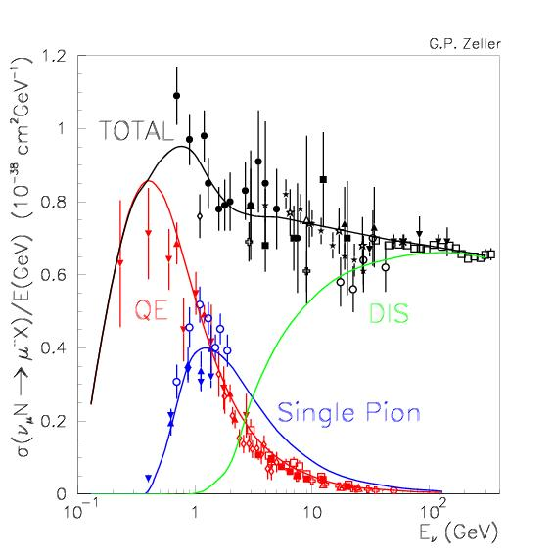
\includegraphics[width=0.9\textwidth]{figures/figs_zeller-total-numode.png}
\caption{Neutrino cross sections, showing the quasi-elastic, deep inelastic and single pion cross sections in the GeV range. Taken from~\cite{82McFarland} modified from original made by G.P.~Zeller~\cite{106Zeller} containing data points from various experiments.}
\label{fig:neutrinoInteractionsFig}
\end{figure}

\begin{figure}[h!]
\centering
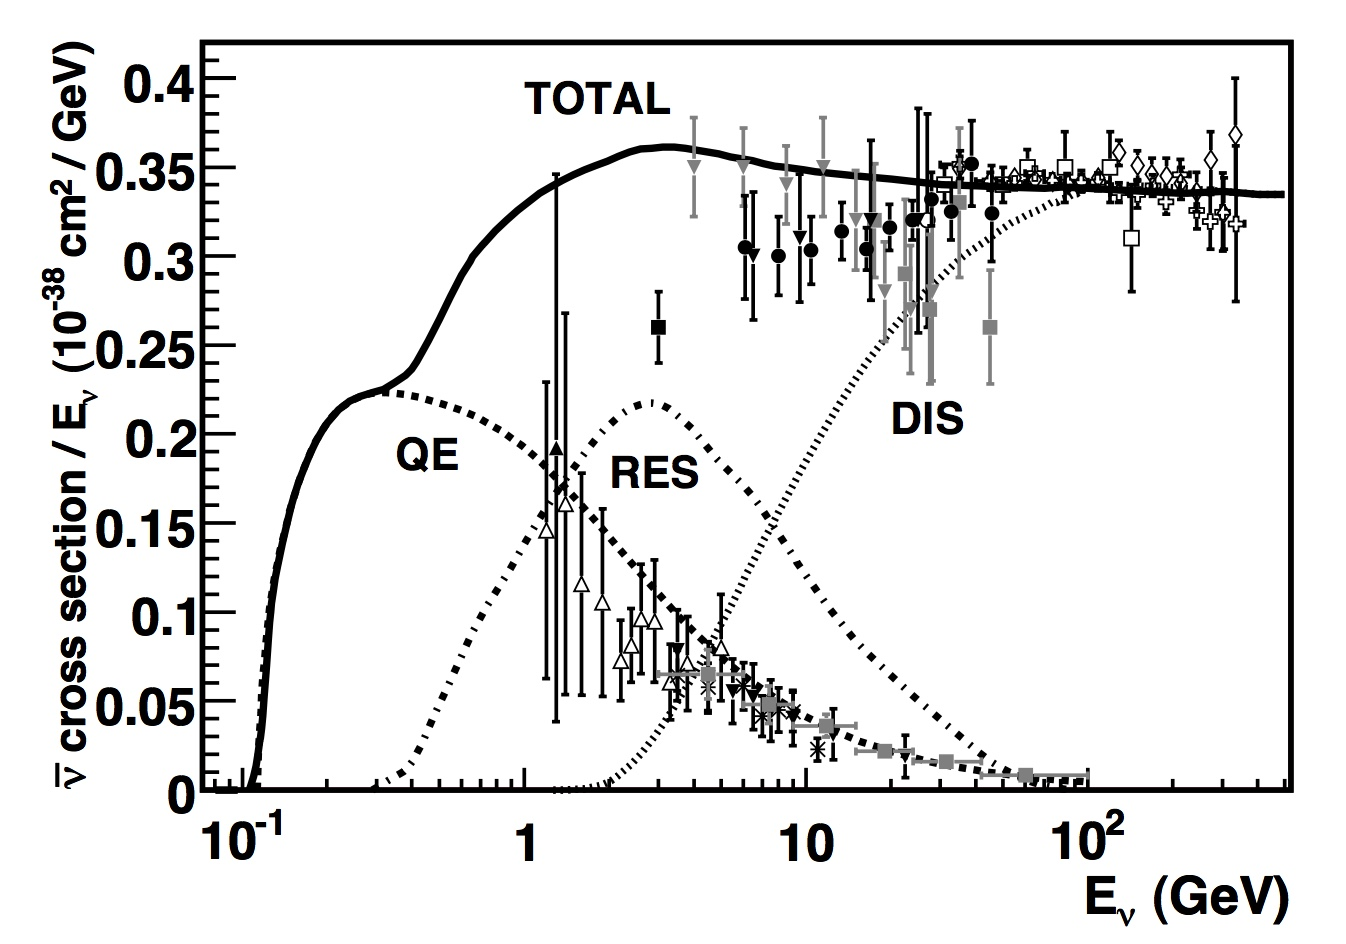
\includegraphics[width=0.9\textwidth]{figures/antineutrinototal.jpeg}
\caption{Antineutrino cross sections, showing the quasi-elastic, deep inelastic and single pion cross sections in the GeV range~\cite{109Formaggio}.}
\label{fig:antineutrinoInteractionsFig}
\end{figure}

The signature for each of these interactions are quite different, as a charge-current quasi-elastic interaction will produce a clean proton and muon track, compared to a shower-like pion track or the less clear DIS signature. Baby MIND is designed to operate at a lower energy spectrum, below 5 GeV, meaning that the contribution will be mostly from CCQE and pion interactions. Results from various simulations with the T2K near detector beam spectrum and data recorded from the commissioning will be shown.

%Lab report again, trying to estimate cross-section of interactions. Why? Need it to improve oscillation measurements. Using simulations of muon neutrinos from simulation. What is done, what cuts? How Do we calculate cross-sections? Angular acceptance, look at what Marc has done, do similar things and further the calculations.Discuss what to expect, what kind of interactions could happen in the TASD/WAGASCI? What could be seen? What information? Baby MIND can also have interactions, which ones would be visible? Can reconstruct muons in Baby MIND, electrons and pions visible and potentially reconstructable, but not now. Charge id, momentum. Identifying muons comming of the neutrino interaction with a specific beam and interaction area. Describe the fiducial volume like in my talk for NuFACT.

\section{Muon charge current quasi-elastic interactions}

Charge current quasi-elastic (CCQE) interactions produce a clear muon track for both neutrinos and antineutrinos, however the interaction only produces a proton track for neutrino interactions as seen below:
\begin{align}
\nu_\mu + n &\rightarrow \mu^- + p\\
 \bar{\nu_\mu} + p &\rightarrow \mu^+ + n
\end{align}

For the neutrino interactions, this becomes a very clear signature in a fully active target where both a muon and proton track can be identified. For antineutrinos this is not possible since neutron tracks are usually not detectable for most detector types.
There have been a lot of interesting articles relating to how to identify neutrino events in argon detectors using machine learning~\cite{83Radovic2018}~\cite{84Adams}. In a non-active target it becomes very difficult to identify neutrino interactions as pions may decay to muons or they may interact in the material and become indistinguishable from directly produced muons.

%Direct simulations with CCQE and different geometries. Use data from specifically Baby MIND in B2 beam line. Explain the beam line etc etc.

%CCQE from muon neutrino produces a muon. Clear production and easy to identify in TASD, not possible in MIND due to the design. 

%Acceptance study, detector layout. Beam settings? Add charge reconstruction, momentum reconstruction. Particle ID? also need interaction ID from TMVA.

%Different size gap, different detector layout both early/testbeam and new at Japan. Cross-section studies. Look at what Marc has done!  Discuss with paul what and how to do cross-section measurements.

\pagebreak
%\subsection{Interactions in TASD + Baby MIND}
\section{Neutrino interactions in a TASD and Baby MIND configuration with a NuSTORM beam}

As described in subsection~\ref{subsec:NuSTORM}, a first stage towards a neutrino factory would contain a storage ring for neutrino and antineutrino production from muon decay. From a muon decay both muon and anti-electron neutrinos will be produced at $\approx 100\%$. In order to evaluate the sensitivity of NuSTORM to the study of neutrino interactions, the TASD and Baby MIND were used as a near detector to measure the interaction type and reconstruction of muon tracks. The main purpose of the study is to see if it is possible to identify muon neutrino CCQE interactions and distinguish them from a background of neutral current interactions and anti-electron charge current interactions. This study was performed using a TMVA trained algorithm with simulated samples. As part of this study the fitted efficiency and charge identification efficiency of negative and positive muon tracks produced by simulated muon neutrinos and antineutrinos in Baby MIND are shown.

The NuSTORM neutrino energy spectrum from the decay of $\mu^-$ has been simulated as can be seen in \FigRef{fig:NuSTORMeSpectrum} for both muon neutrinos and anti-electron neutrinos. This is the spectrum of neutrino flavours observed in a detector at a distance of 50~m from the end of the NuSTORM straight section (as shown in \FigRef{fig:nuStorm}). The main job for any detector will be to identify if the neutrino event is produced from either a $\nu_\mu$ CC interaction, producing a $\mu^-$, or from a $\bar{\nu}_e$ interaction, which produces positrons, as well as dealing with the neutral current (NC) background from all neutrinos.
%muon interaction or an electron interaction as well as dealing with the small background ($<1\%$) of anti-muon produced electron and anti-muon neutrinos.

\begin{figure}[h!]
\centering
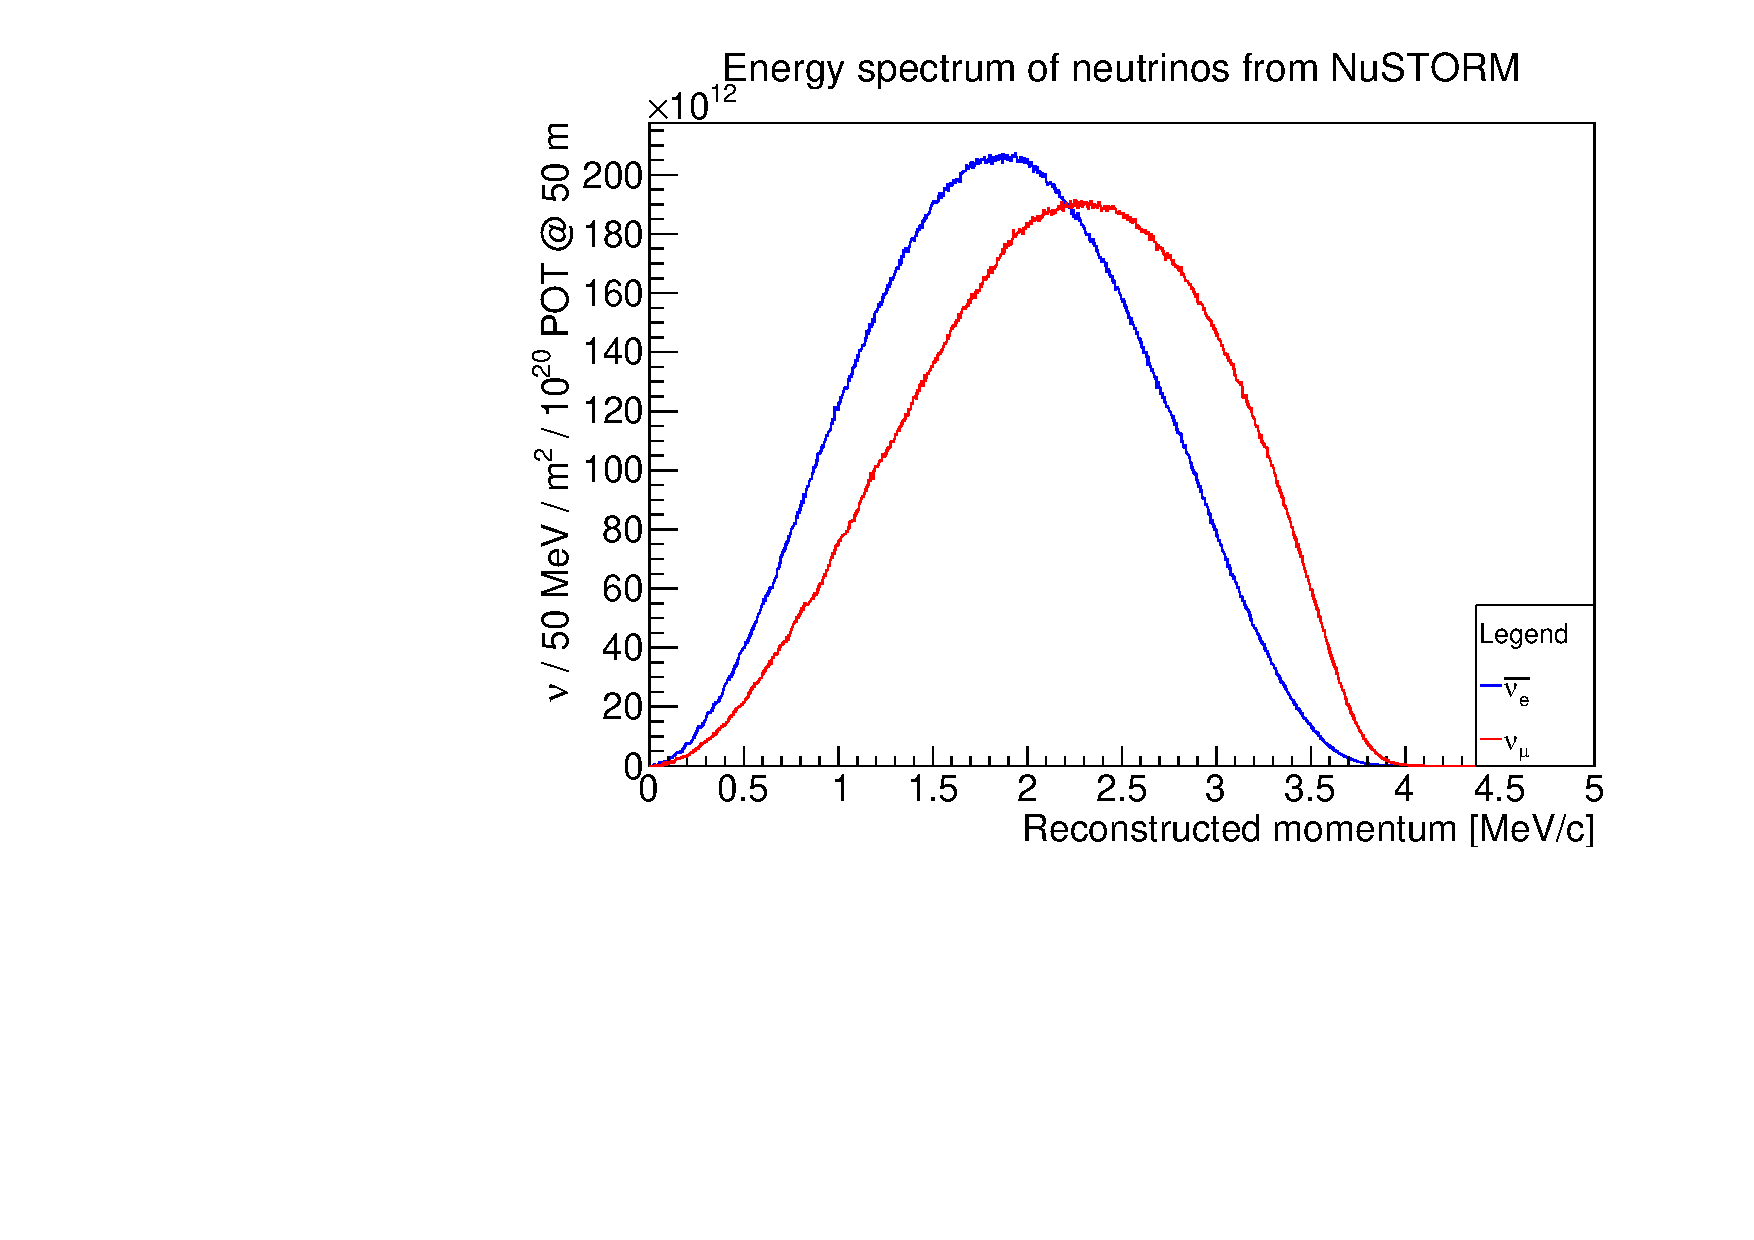
\includegraphics[width=0.9\textwidth]{figures/eSpectrum.pdf}
\caption{Energy spectrum of muon neutrinos and anti-electron neutrinos produced at NuSTORM and recorded at 50 m from the storage ring.}
\label{fig:NuSTORMeSpectrum}
\end{figure}

During the construction of Baby MIND, it was proposed to fully instrument the whole TASD, used during the first beam test, and use it as a fully active target to be combined with Baby MIND, illustrated in~\FigRef{fig:TASDandMIND}. This could become a setup for a NuSTORM detector.

\begin{figure}[h!]
\centering
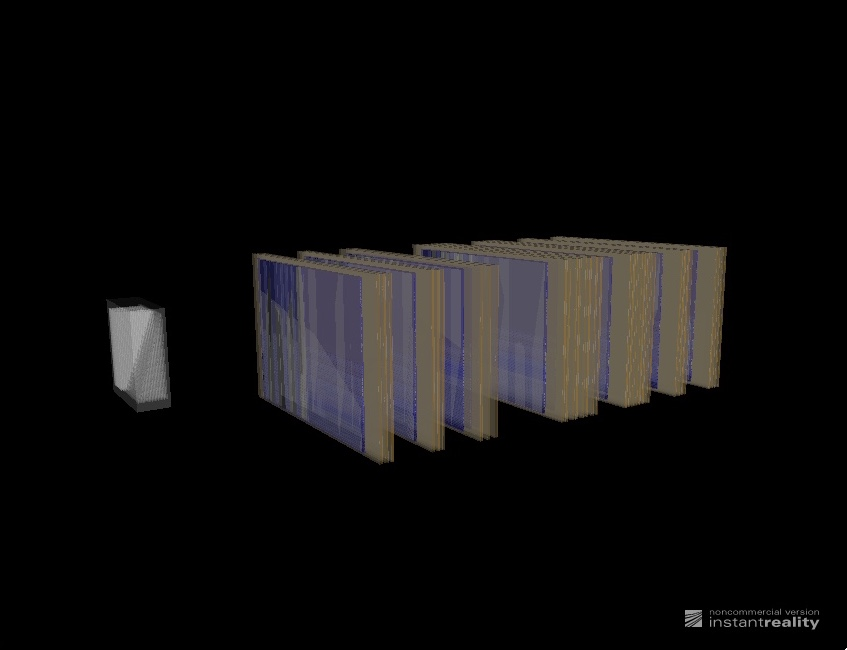
\includegraphics[width=0.9\textwidth]{figures/MINDAida.jpeg}
\caption{An illustrative sketch of the detector setup with the TASD detector in front of Baby MIND.}
\label{fig:TASDandMIND}
\end{figure}

Using the SAURON framework, $10^5$ muon neutrinos and muon antineutrinos were simulated using the NuSTORM energy spectrum and reconstructed to provide the figures of merit presented below. In \FigRef{fig:NuSTORMTASDfitted} the reconstruction efficiency is presented, \FigRef{fig:NuSTORMTASDfittedcharge} shows the charge efficiency and finally \FigRef{fig:NuSTORMTASDCombined} shows these two multiplied. Each of the plots show different metrics to evaluate the SAURON framework and the detector performance. The reconstruction efficiency is defined as the ratio of reconstructible tracks divided by all the simulated tracks. The charge efficiency is defined as how many of the reconstructible tracks are reconstructed with the correct charge. Multiplying these two results gives the ratio of reconstructed tracks with the correct charge divided by all simulated tracks.

\begin{figure}[h!]
\centering
%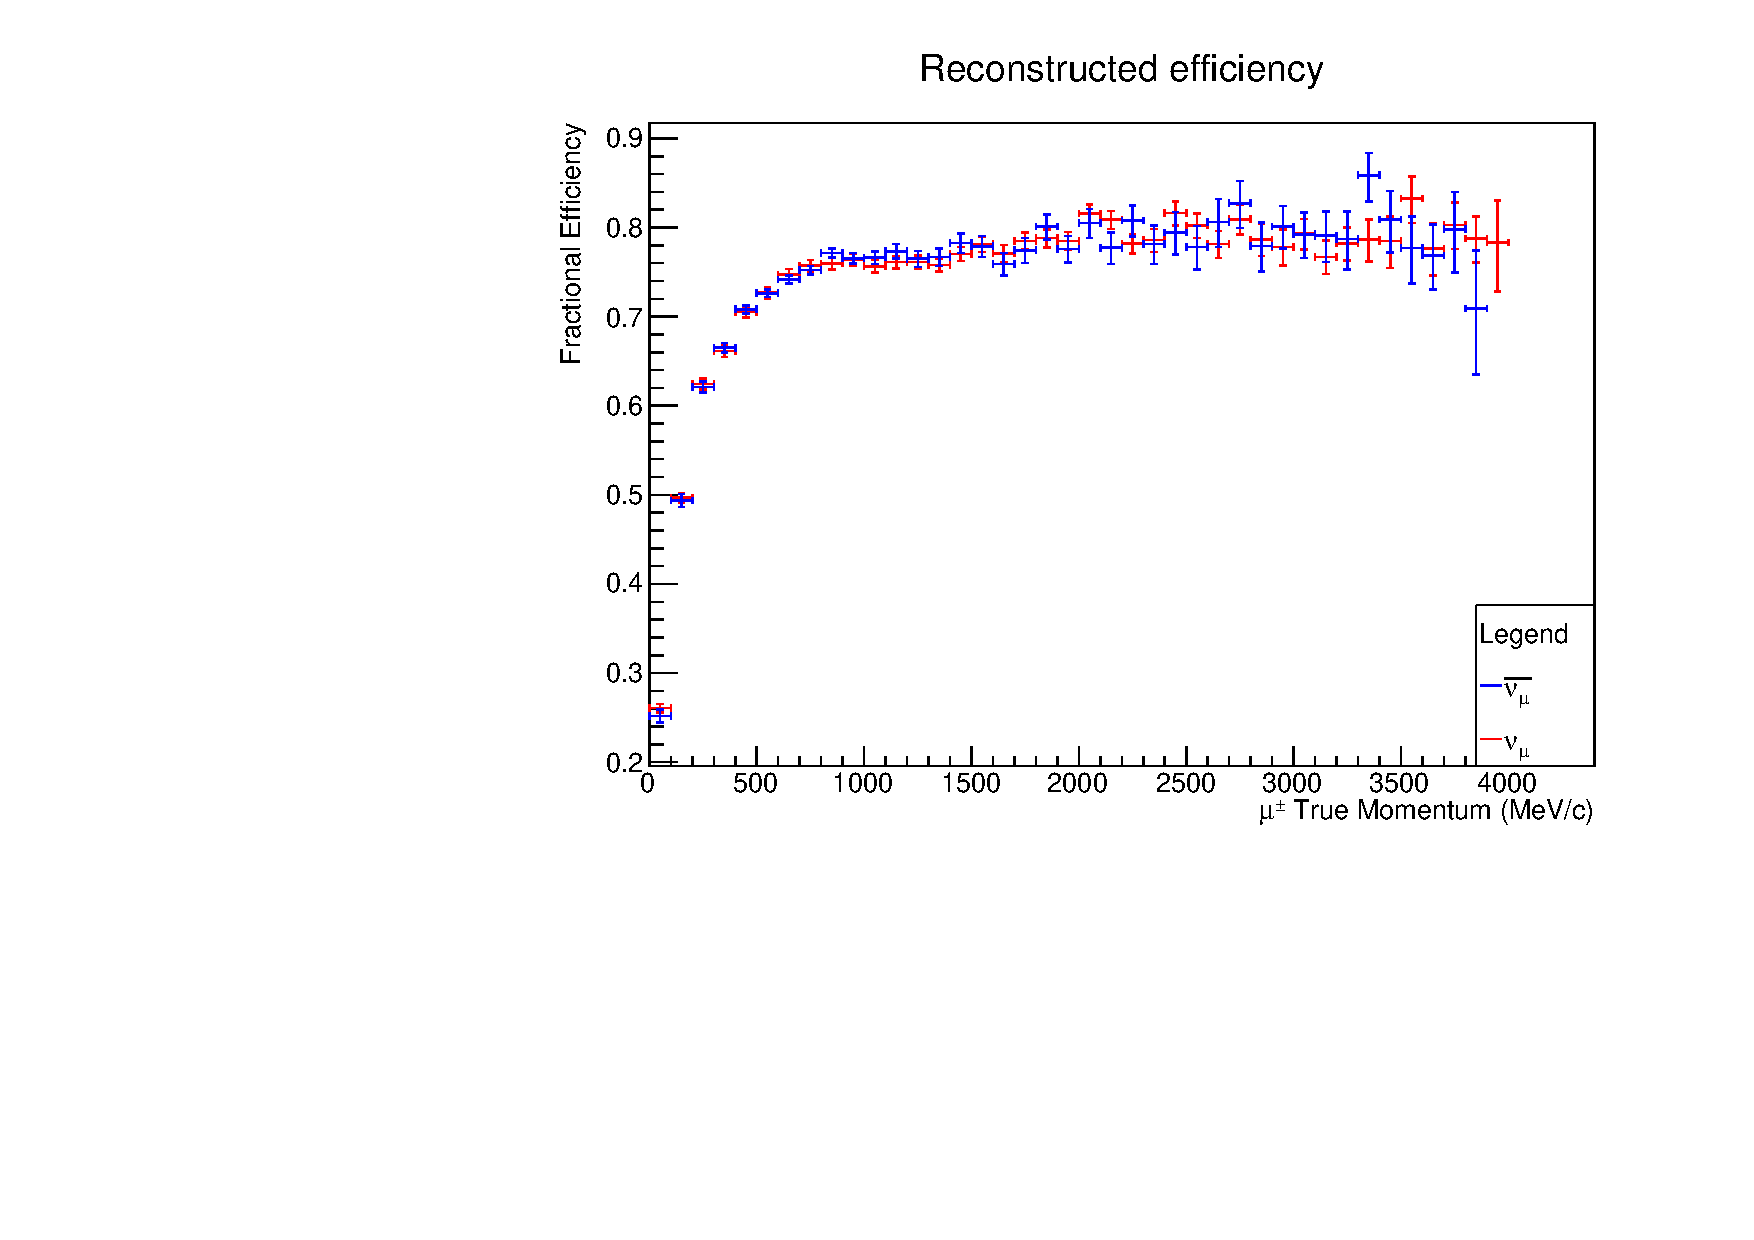
\includegraphics[width=.9\textwidth]{figures/NeutrinoChap/data260618/T2K/FittedT2KNeutrinoBeamMIND.pdf}
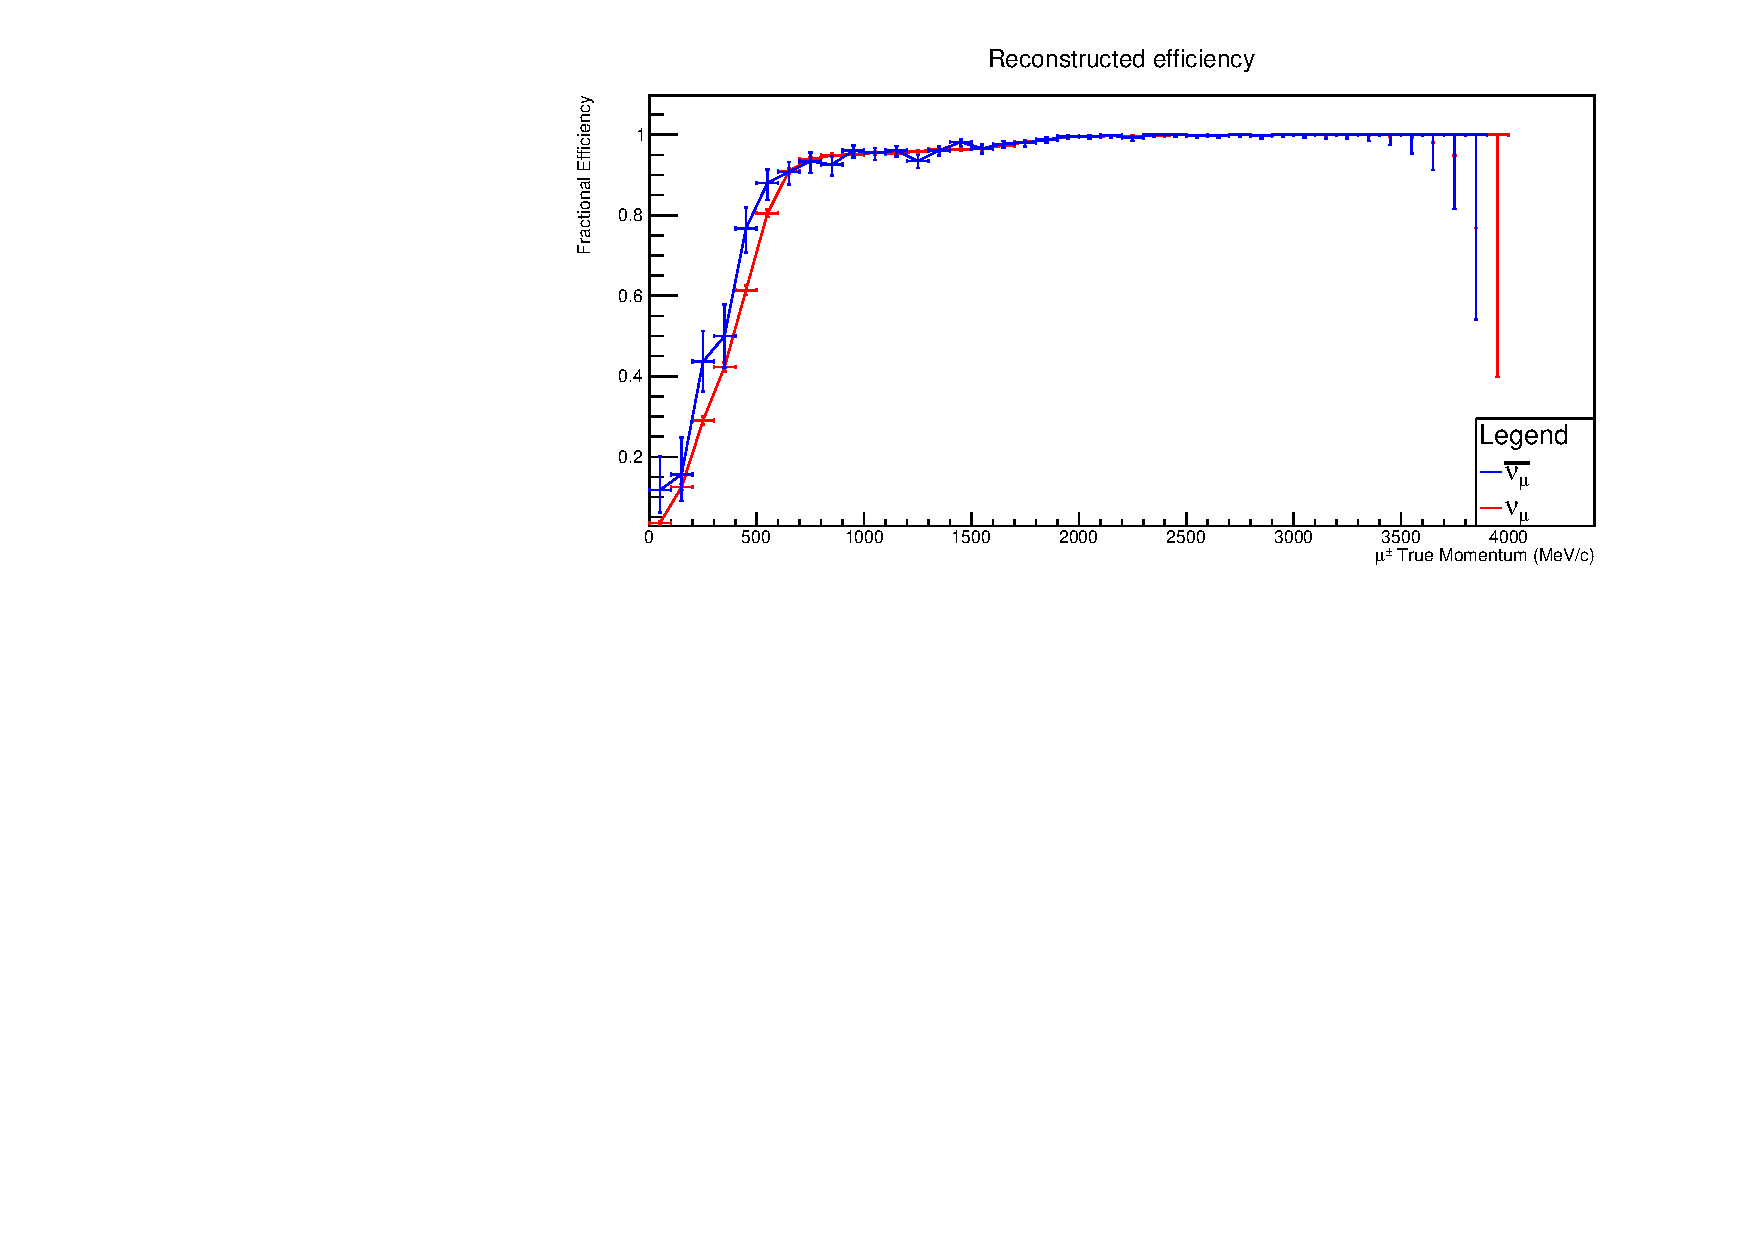
\includegraphics[width=.9\textwidth]{figures/NeutrinoChap/Neutrino/NuStormRecEff.pdf}
\caption{The efficiency plot of how well the SAURON algorithm can reconstruct muon tracks from neutrino interactions simulated with the NuSTORM beam as a function of muon momenta.}
\label{fig:NuSTORMTASDfitted}
\end{figure}

\begin{figure}[h!]
\centering
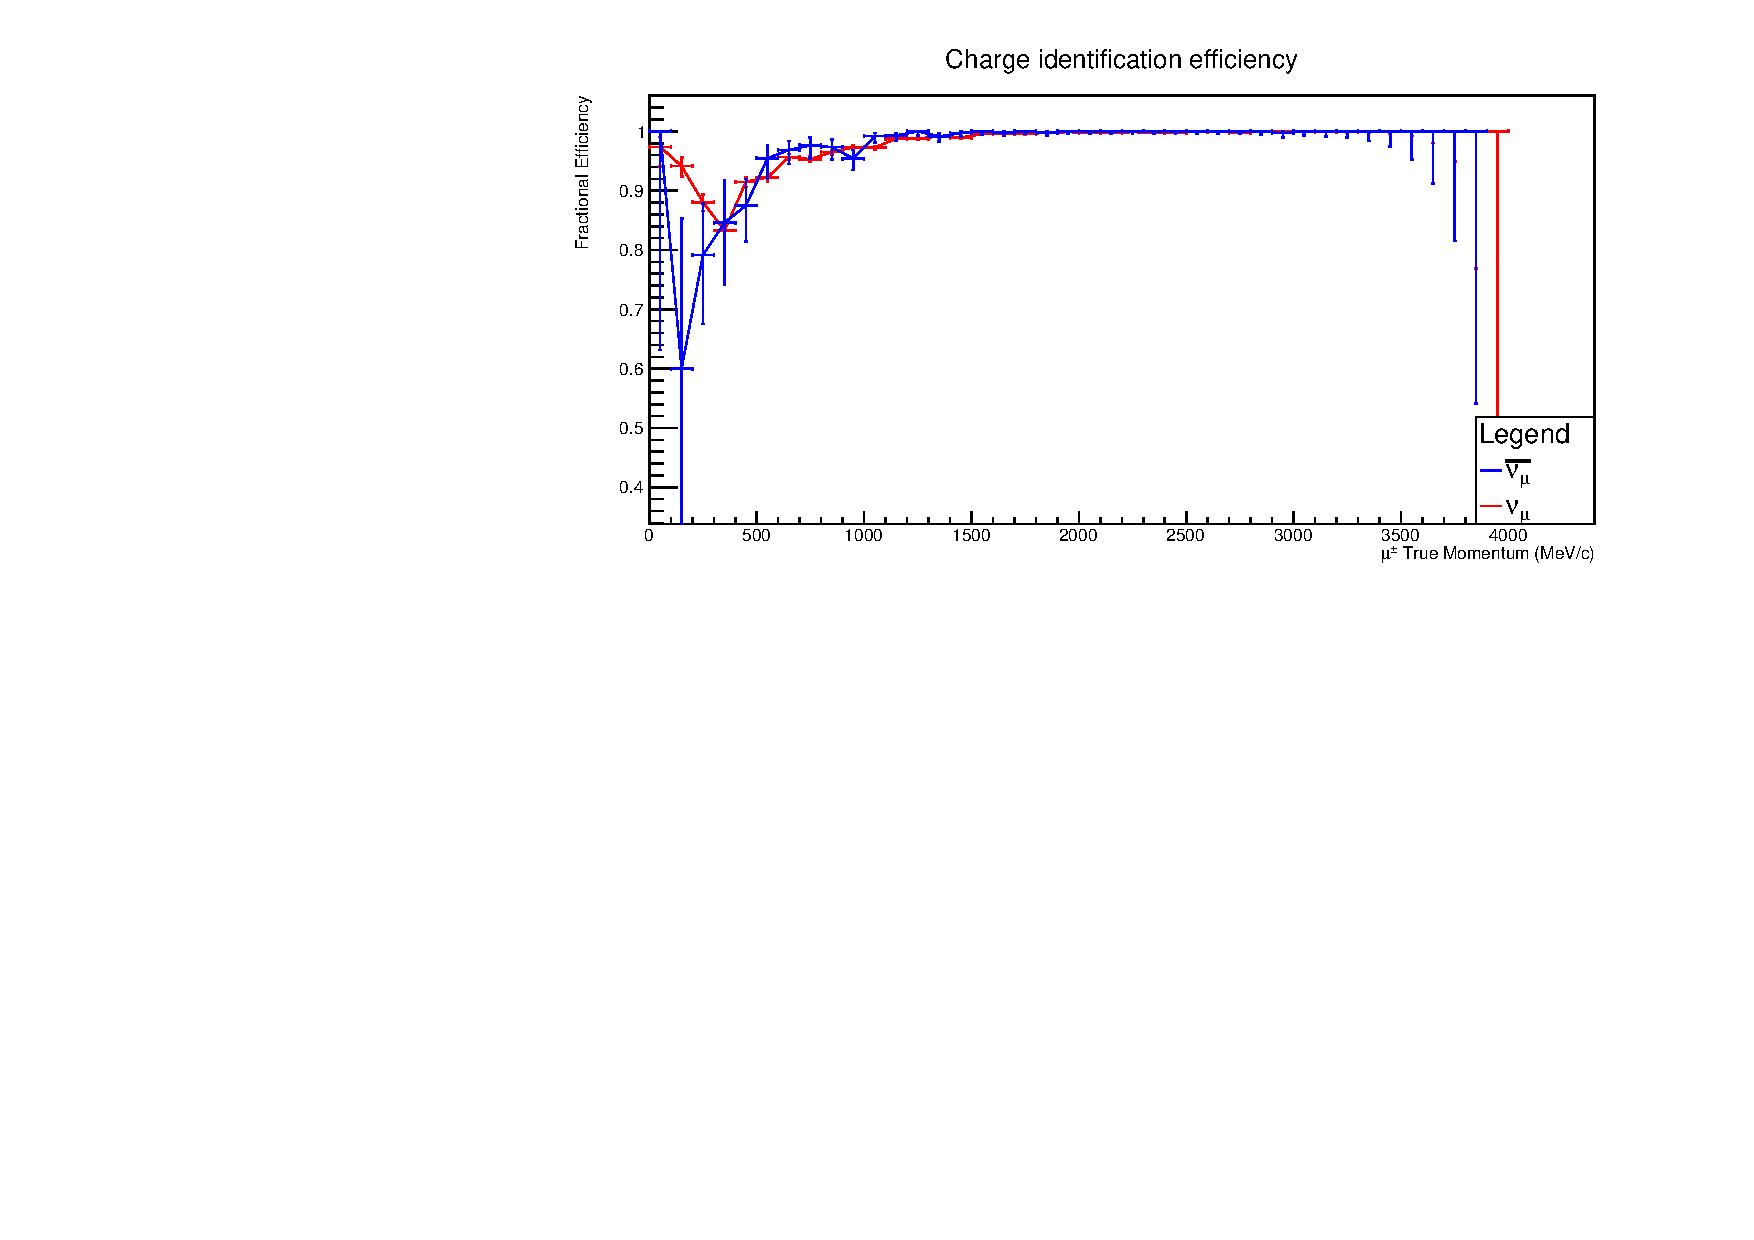
\includegraphics[width=.9\textwidth]{figures/NeutrinoChap/Neutrino/NuStormChargeEff.pdf}
%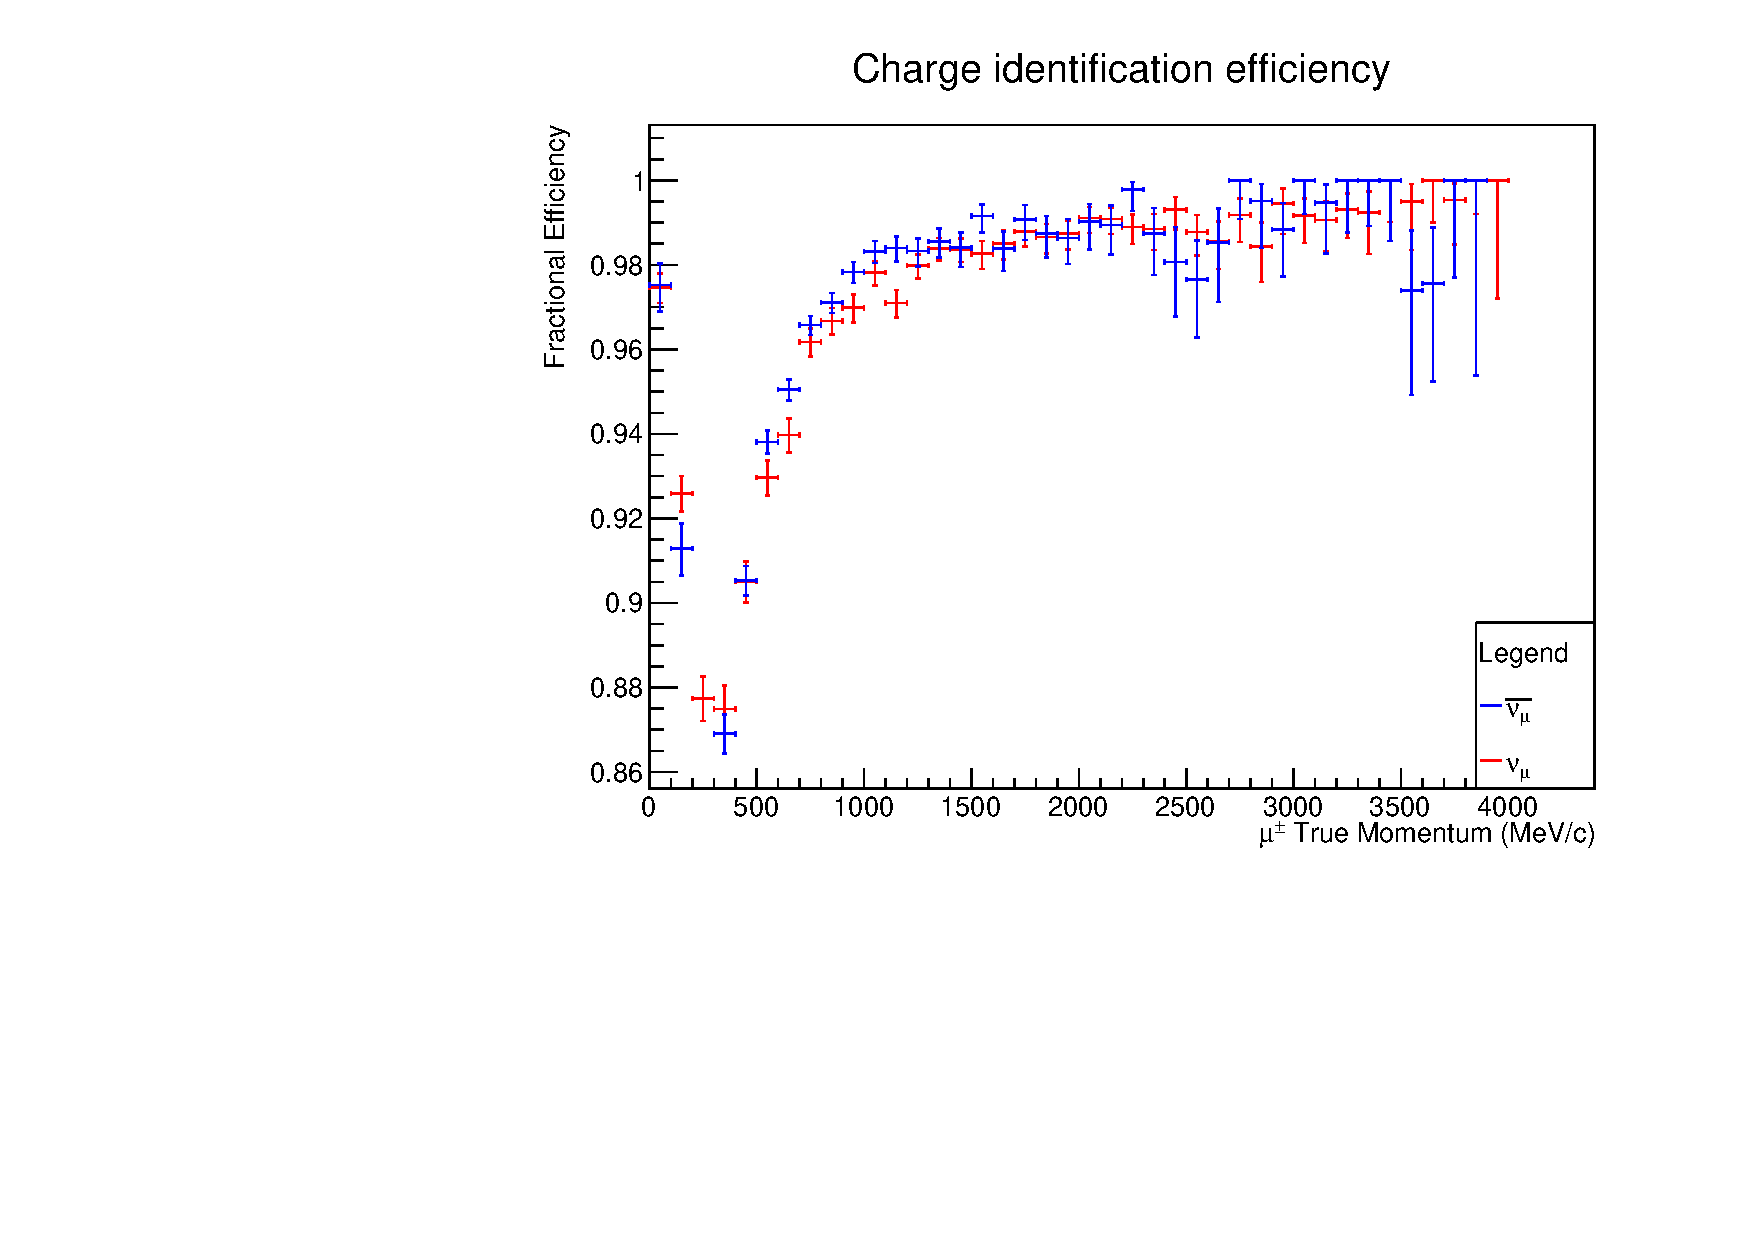
\includegraphics[width=.9\textwidth]{figures/NeutrinoChap/data260618/T2K/ChargeIDT2KNeutrinoBeamMIND.pdf}
\caption{The efficiency plot of how well the SAURON algorithm can reconstruct the charge from reconstructed muon tracks from neutrino interactions simulated with the NuSTORM beam as a function of muon momenta.}
\label{fig:NuSTORMTASDfittedcharge}
\end{figure}

\begin{figure}[h!]
\centering
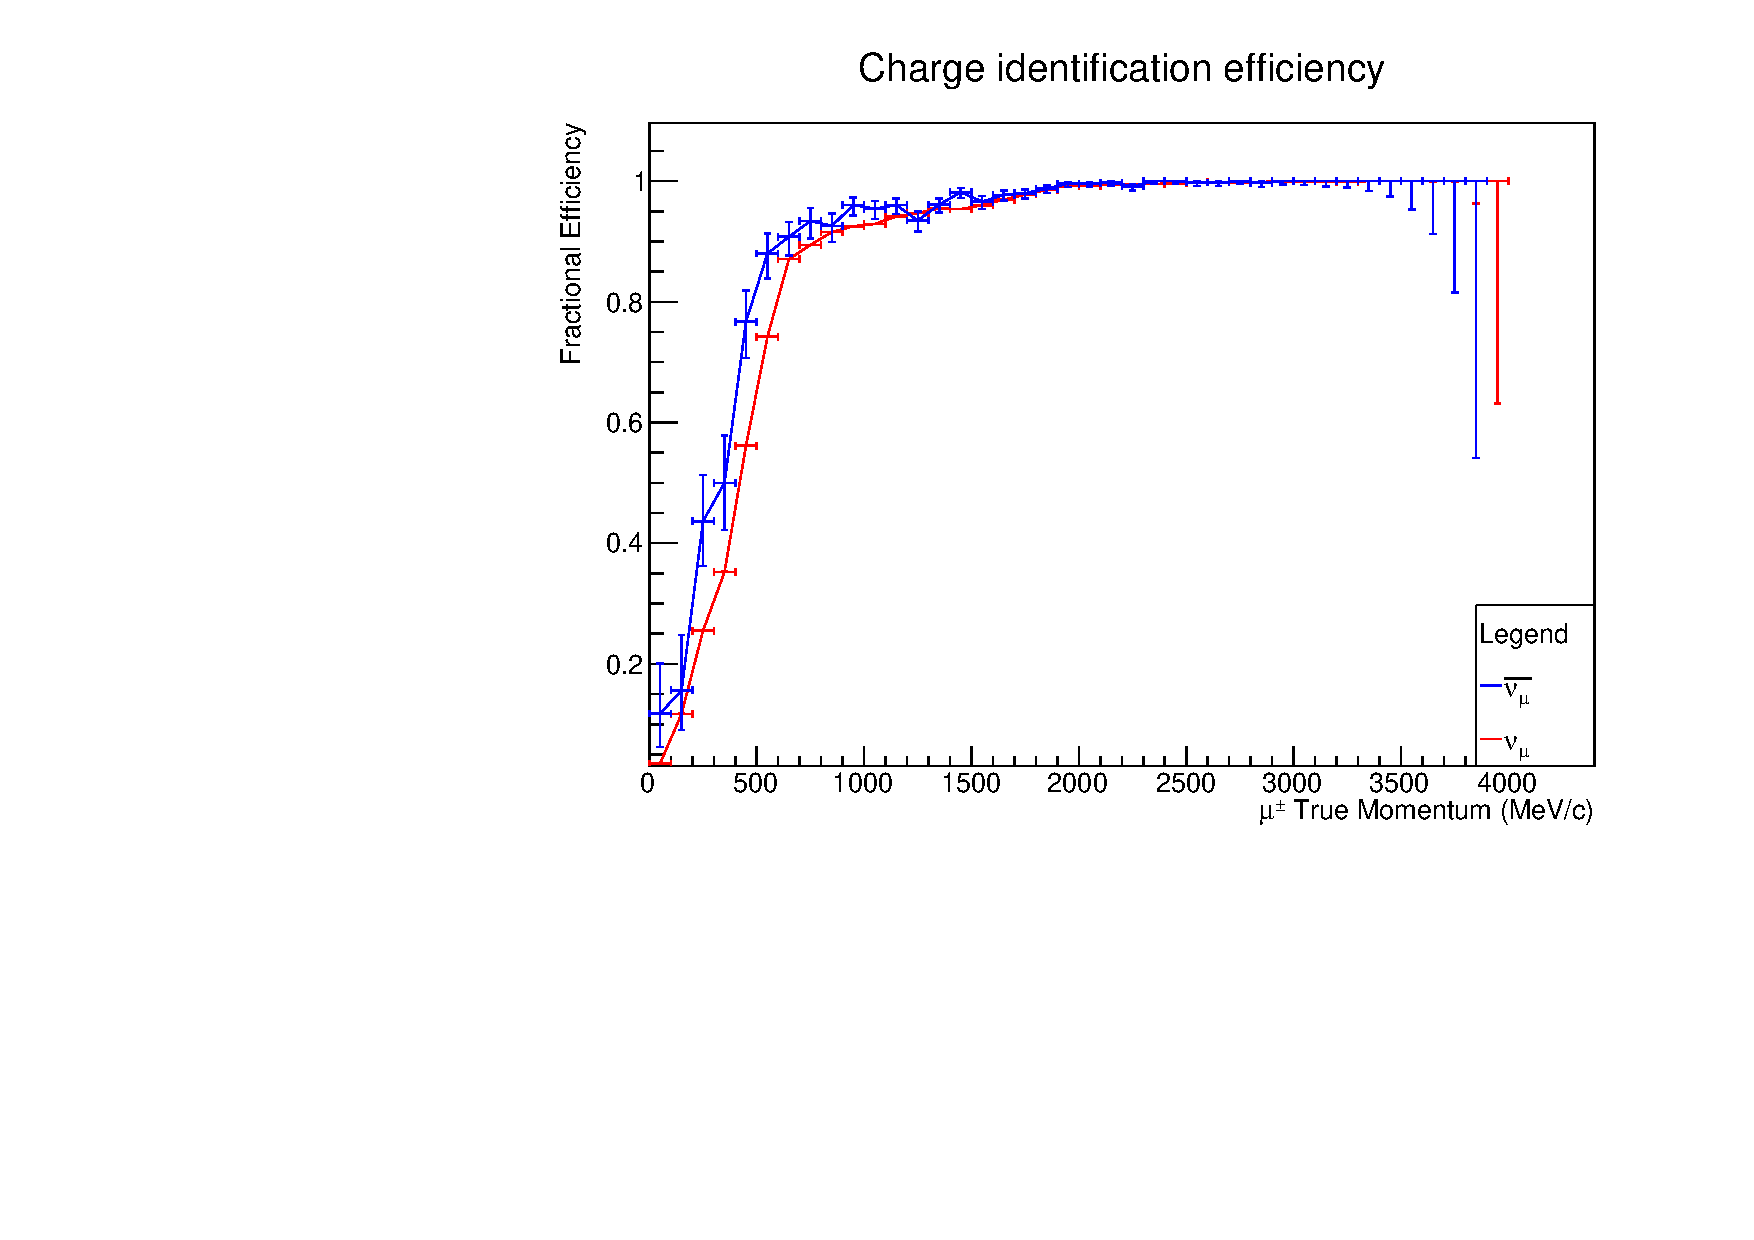
\includegraphics[width=.9\textwidth]{figures/NeutrinoChap/CombinedNuStormChargeFittedEff.pdf}
%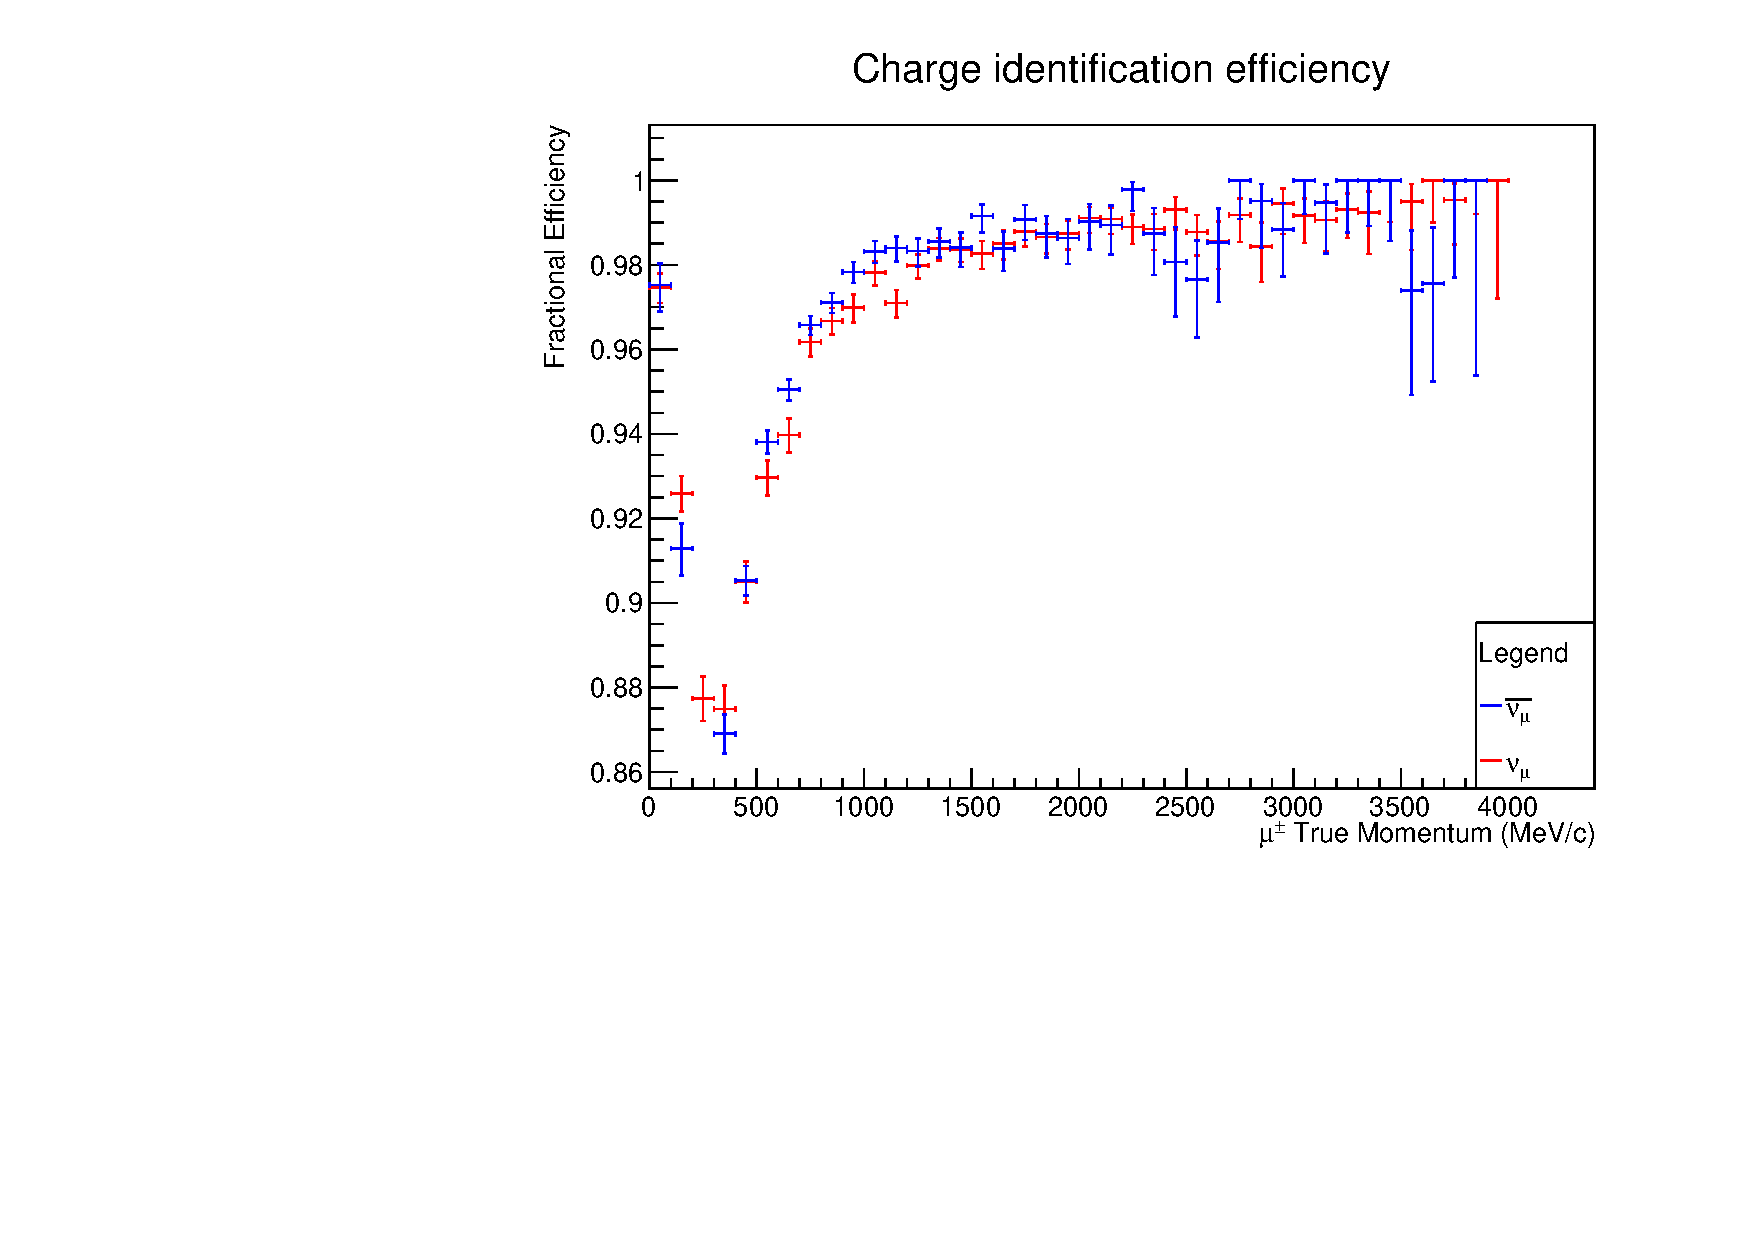
\includegraphics[width=.9\textwidth]{figures/NeutrinoChap/data260618/T2K/ChargeIDT2KNeutrinoBeamMIND.pdf}
\caption{The efficiency plot of how well the SAURON algorithm can reconstruct the charge from muon tracks with respect to all the simulated neutrino interactions with the NuSTORM beam as a function of muon momenta. This plot is the multiplication of the efficiencies in \FigRef{fig:NuSTORMTASDfitted} and \FigRef{fig:NuSTORMTASDfittedcharge}.}
\label{fig:NuSTORMTASDCombined}
\end{figure}

%Similarly to the simulated muon beam, and data the charge reconstruction efficiency is very good for the reconstructible tracks.
Similarly to the studies carried out in chapter 5 for single muons in the CERN test beam, the charge reconstruction efficiency of muons from neutrino charge current interactions, using the NuSTORM beam, is very high, even at low momenta. The main difference arises from the fact that the neutrinos are produced at a variety of angles with respect to the neutrino direction instead of straight on the center of the detector (with some beam size). Muons from neutrinos are produced at different angles depending on the kinematics of the neutrino interaction and neutrino energy. 

\section{Neutrino event selection from the NuSTORM beam}

%This is written without context. Here you need to introduce the event selection of the NuSTORM beam and justify how many events we are expected to get for a detector of the size of the TASD. It could be something like:

The NuSTORM beam produces $\nu_\mu$ and $\bar{\nu}_e$ neutrinos from the decay of muons, $ \mu^- \rightarrow e^- + \nu_\mu + \bar{\nu}_e $ according to the energy distribution in~\FigRef{fig:NuSTORMeSpectrum}. These neutrinos can produce both CC and NC events in the TASD in front of Baby MIND. It is important to separate the $\nu_\mu$ CCQE interactions from the NC and $\bar{\nu}_e$ background to perform analysis of CCQE events. A machine learning multi-variate analysis was carried out to perform the event selection, using the TMVA package. The variables used to populate the TMVA algorithm are similar to the particle identification study carried out in chapter 5.

%For the TMVA algorithm, similar variables to the muon, pion study for the test beam as to simplify the implementation.

The main variables used in the model are the following:
\begin{itemize}
\item Maximum distance between hits in an event (MC\_ track\_ len),
\item Angle of the track compared to the $z$-axis that defines the length of the detector\\ (MC\_ angle),
\item Number of total hits in the event (NumberofHits),
\item Number of planes hit (NumberofPlanes),
\item Average number of hits per plane (AvrHitsPerPlane).
%\item Number of total hits,
%\item Number of used planes for fit
%\item Number of hits used for fit/ number of used planes
%\item Average number of hits per plane
%\item Maximum distance between hits in an event / Naive track length
\end{itemize}

The distributions of these variables for signal and background can be seen in \FigRef{fig:TMVANeuinput}.


\begin{figure}[h!]
\centering

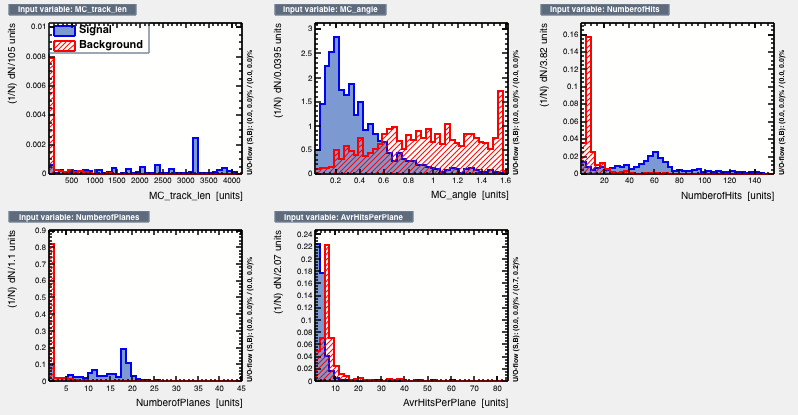
\includegraphics[width=\textwidth]{figures/neutrinoTMVA/variables_id_c1.png}
\caption{Input variables for both signal and background using simulated data.}
\label{fig:TMVANeuinput}
\end{figure}

Based on these simulated signal and background samples, TMVA will provided a signal efficiency curve based on the various built-in machine learning models, seen in \FigRef{fig:TMVANeuroc}. In this plot is is clear that several models outperform others, however the multilayer perceptron with a Bayesian Neural Network (MLPBNN) was chosen as the best performing model. The MLPBNN response can be seen in \FigRef{fig:TMVANeuresponce} and shows a clear distinction between signal and background samples. It is quite clear that any cut between these two distinct peaks will produce the desired outcome, this is plotted in \FigRef{fig:TMVANeucuts}. For this study the significance is chosen as the possibility to see a signal over the background as $S/\sqrt{S+B}$, where $S$ is the number of signal events and $B$ is the number of background events, which is a figure-of-merit often used in particle physics. The background is chosen to be close to the estimated interaction probability. For 1000 $\nu_\mu$ CC signal events, there are 1000 $\bar{\nu}_e$ CC events and 333 $\nu_\mu$ NC events and 333 $\bar{\nu}_e$ NC events. This provides a total of 1666 background events for 1000 signal events.
 %and shows the ideal value if the number of signal and background events are equal.

%Explain the details of figure 6.11, say where you put your optimised cut and how you optimise with a figure of merit S/sqrt(S+B).

%Also, does the background include a mixture of NC and \bar{\nu}_e events? If it does, what percentage of background is NC and what percentage is \bar{\nu}_e?

%It really should not be equal amount of signal and background. If the $\nu_\mu$ CC signal is 1, the $\bar{\nu}_e$ CC would also be 1, and the NC from \nu_\mu$ would be 1/3 and the NC from $\bar{\nu}_e$  should also be 1/3. So, if signal is 1, the background should be 1.66.

%Currently found that the best method, however many perform similarly, is MLPBNN, Multilayer perceptron (neutral network) with BFGS training method, similar to gradient decent or quasi-Newton method, and bayesian regulator.


\begin{figure}[h!]
\centering
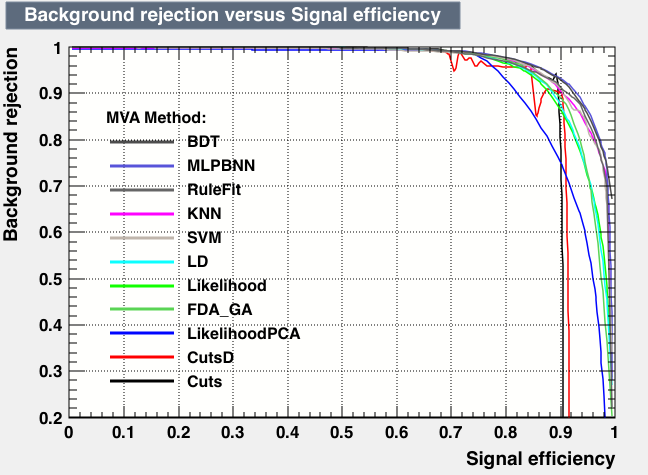
\includegraphics[width=\textwidth]{figures/newTMVAplots/rejBvsS.png}
%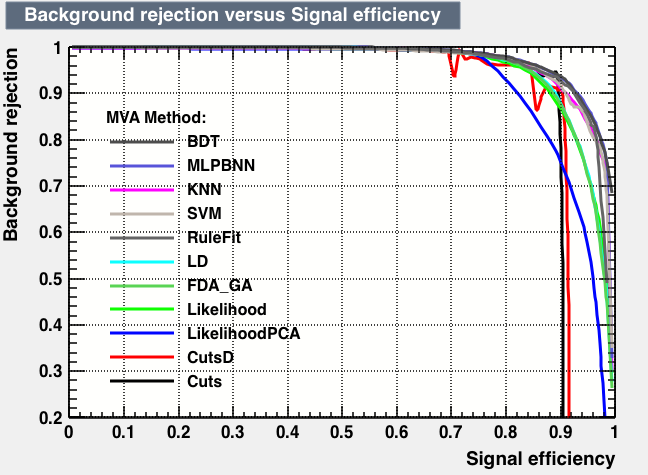
\includegraphics[width=\textwidth]{figures/neutrinoTMVA/rejBvsS.png}
\caption{Receiver operating characteristic (ROC) curve for various machine learning algorithms.}
\label{fig:TMVANeuroc}
\end{figure}

\begin{figure}[h!]
\centering
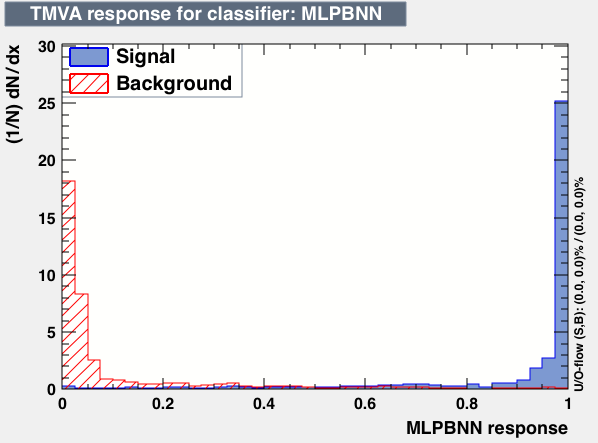
\includegraphics[width=.49\textwidth]{figures/newTMVAplots/mva_MLPBNN.png}
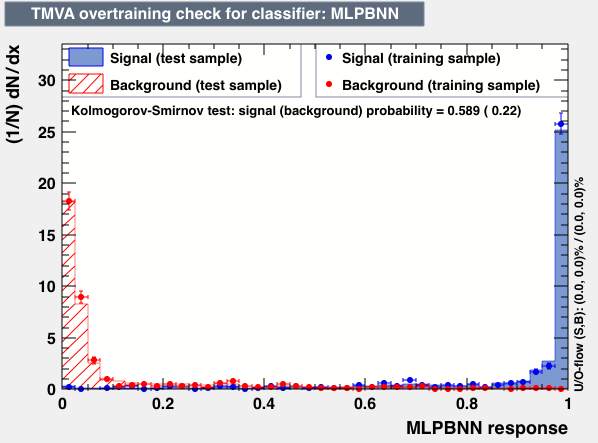
\includegraphics[width=.49\textwidth]{figures/newTMVAplots/overtrain_MLPBNN.png}
%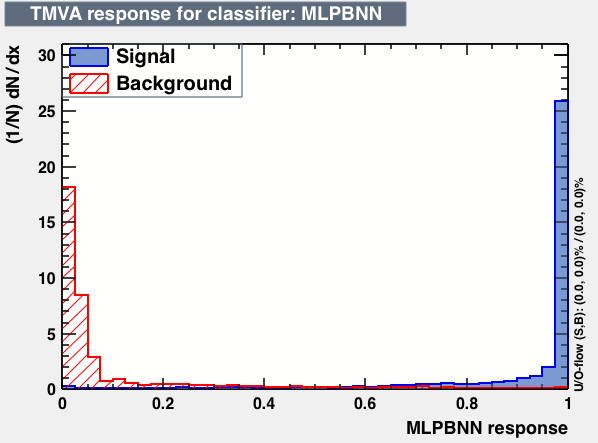
\includegraphics[width=.49\textwidth]{figures/neutrinoTMVA/mva_MLPBNN.png}
%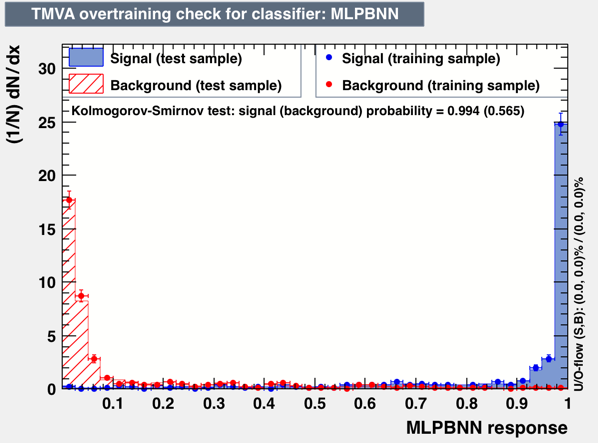
\includegraphics[width=.49\textwidth]{figures/neutrinoTMVA/overtrain_MLPBNN.png}
\caption{Response with and without over-training check.}
\label{fig:TMVANeuresponce}
\end{figure}

With this trained algorithm the best possible cut value (0.50) allows 91\% of the signal events to pass, and only accepts 7.6\% of the background.

%As with the previous study this is done independent of neutrino energy values. 
As with the previous study, this analysis is performed independently of neutrino energy values. This could be tailoring the cuts for specific energy ranges, or by including extra variables in the TMVA study, such as perhaps energy deposited into the scintillating bars in the detector.% however this would require a further study to determine potentially better variables.

Applying the TMVA algorithm to a mixed sample of electron neutrinos and muon neutrinos produces the neutrino energy spectrum seen in \FigRef{fig:TMVAEspectrumAfter} with the initial spectrum seen in \FigRef{fig:TMVAEspectrumBefore} providing a signal efficiency of 84\%.

%Make further comments here that the background is reduced from x% to y%.

\begin{figure}[h!]
\centering

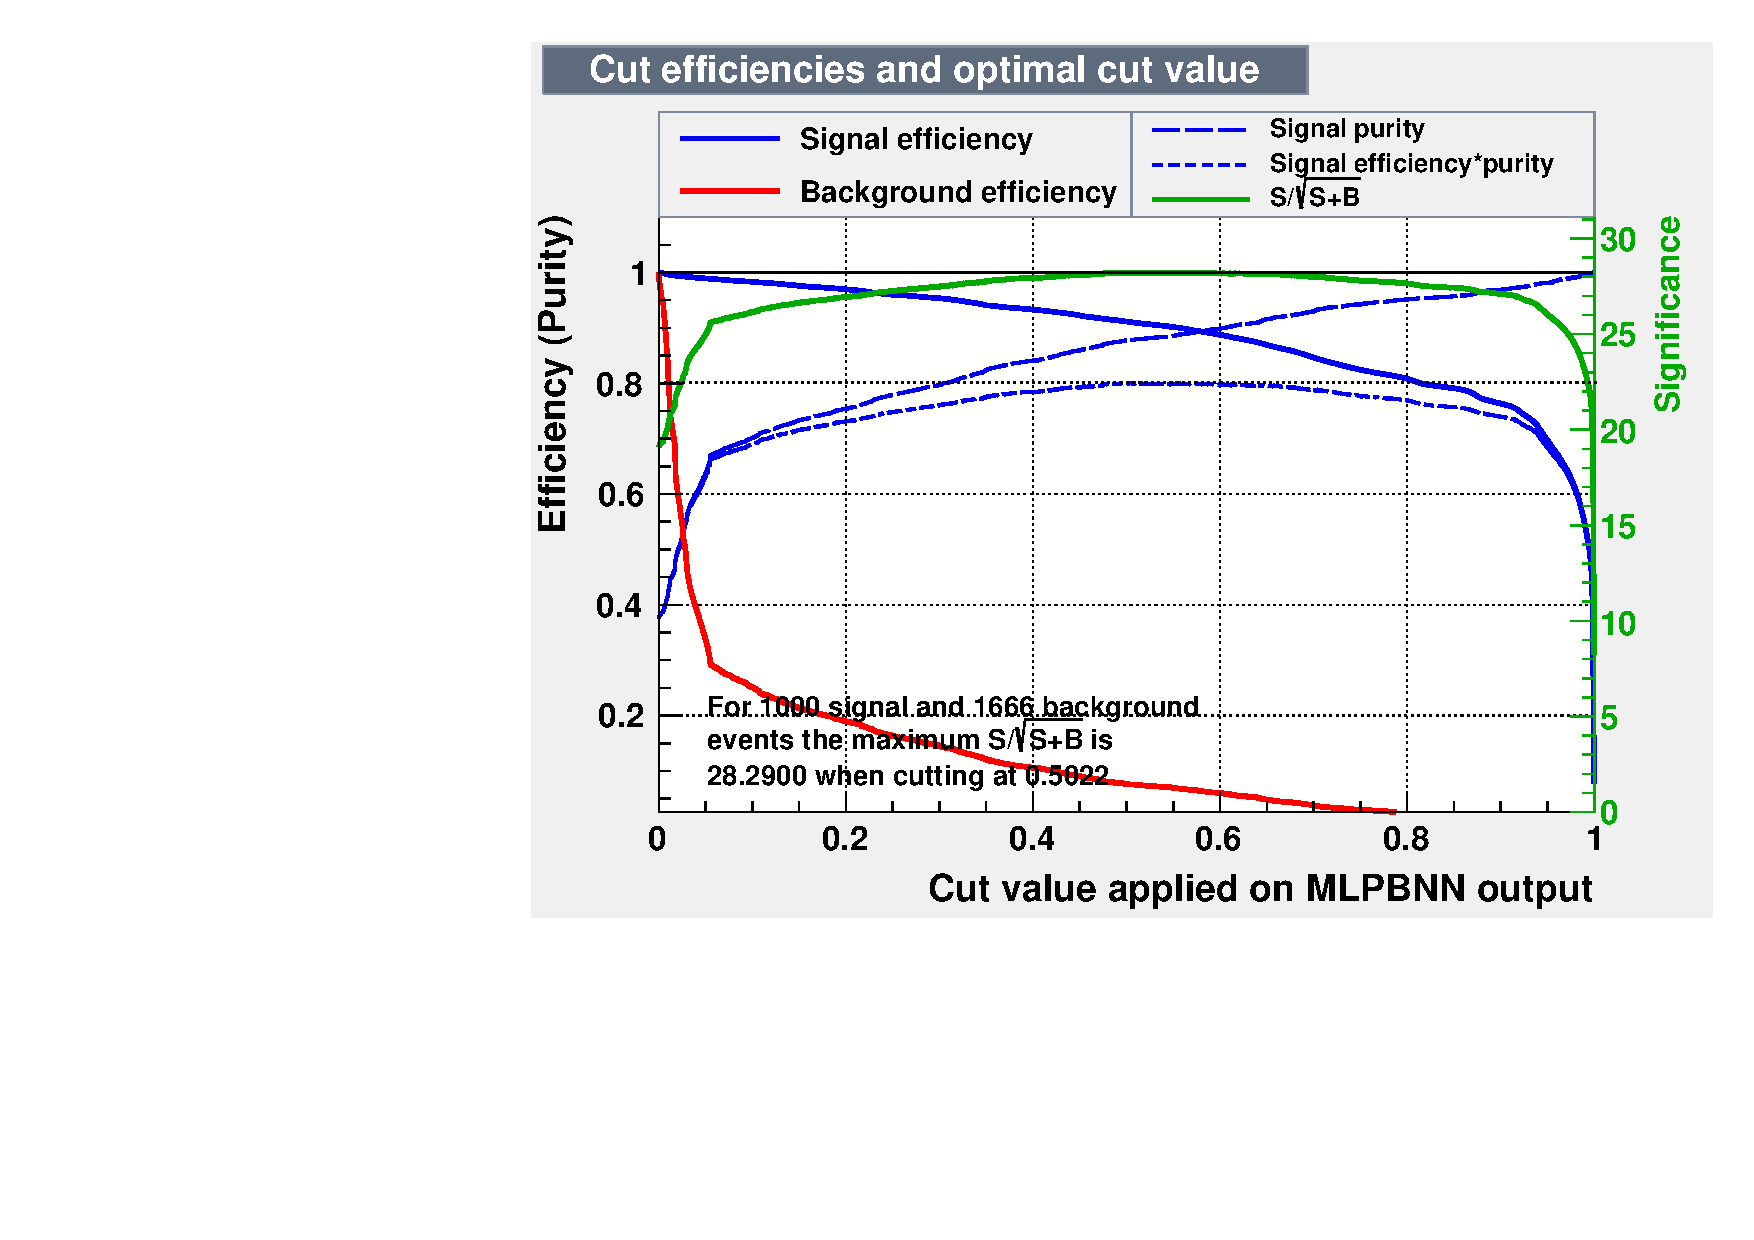
\includegraphics[width=\textwidth]{figures/newTMVAplots/CorrCutMLPBNN.pdf}
%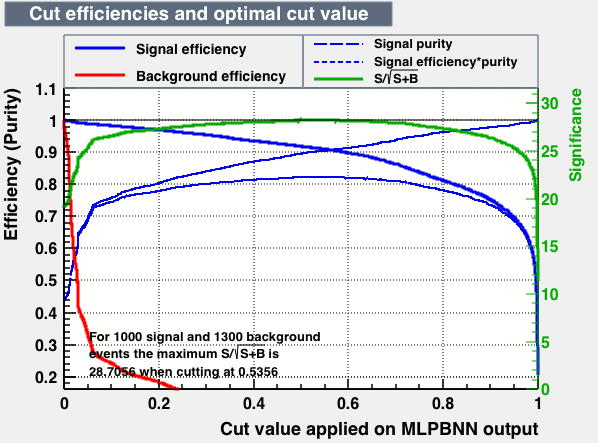
\includegraphics[width=\textwidth]{figures/NeutrinoChap/mvaeffs_MLPBNN10001300.png}
%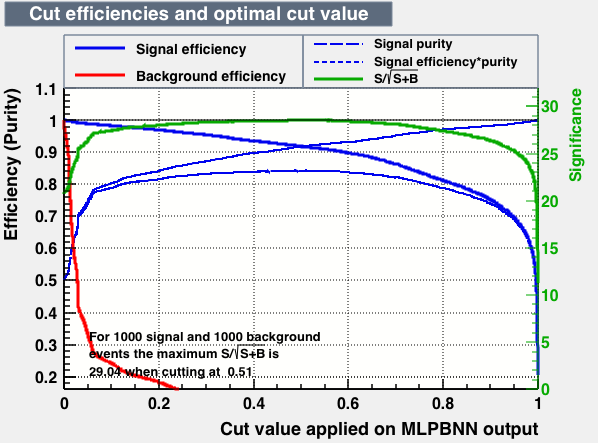
\includegraphics[width=\textwidth]{figures/neutrinoTMVA/mvaeffs_MLPBNN.png}
\caption{Cut efficiency plots expecting the combined background of $\bar{\nu}_{eCC}$ to be at the same number as the signal ($\nu_{\mu_{CC}}$) and $\nu_{\mu_{NC}}$ to be approximately $\frac{2}{3}$ of the number of signal events. }
\label{fig:TMVANeucuts}
\end{figure}

\begin{figure}[h!]
\centering
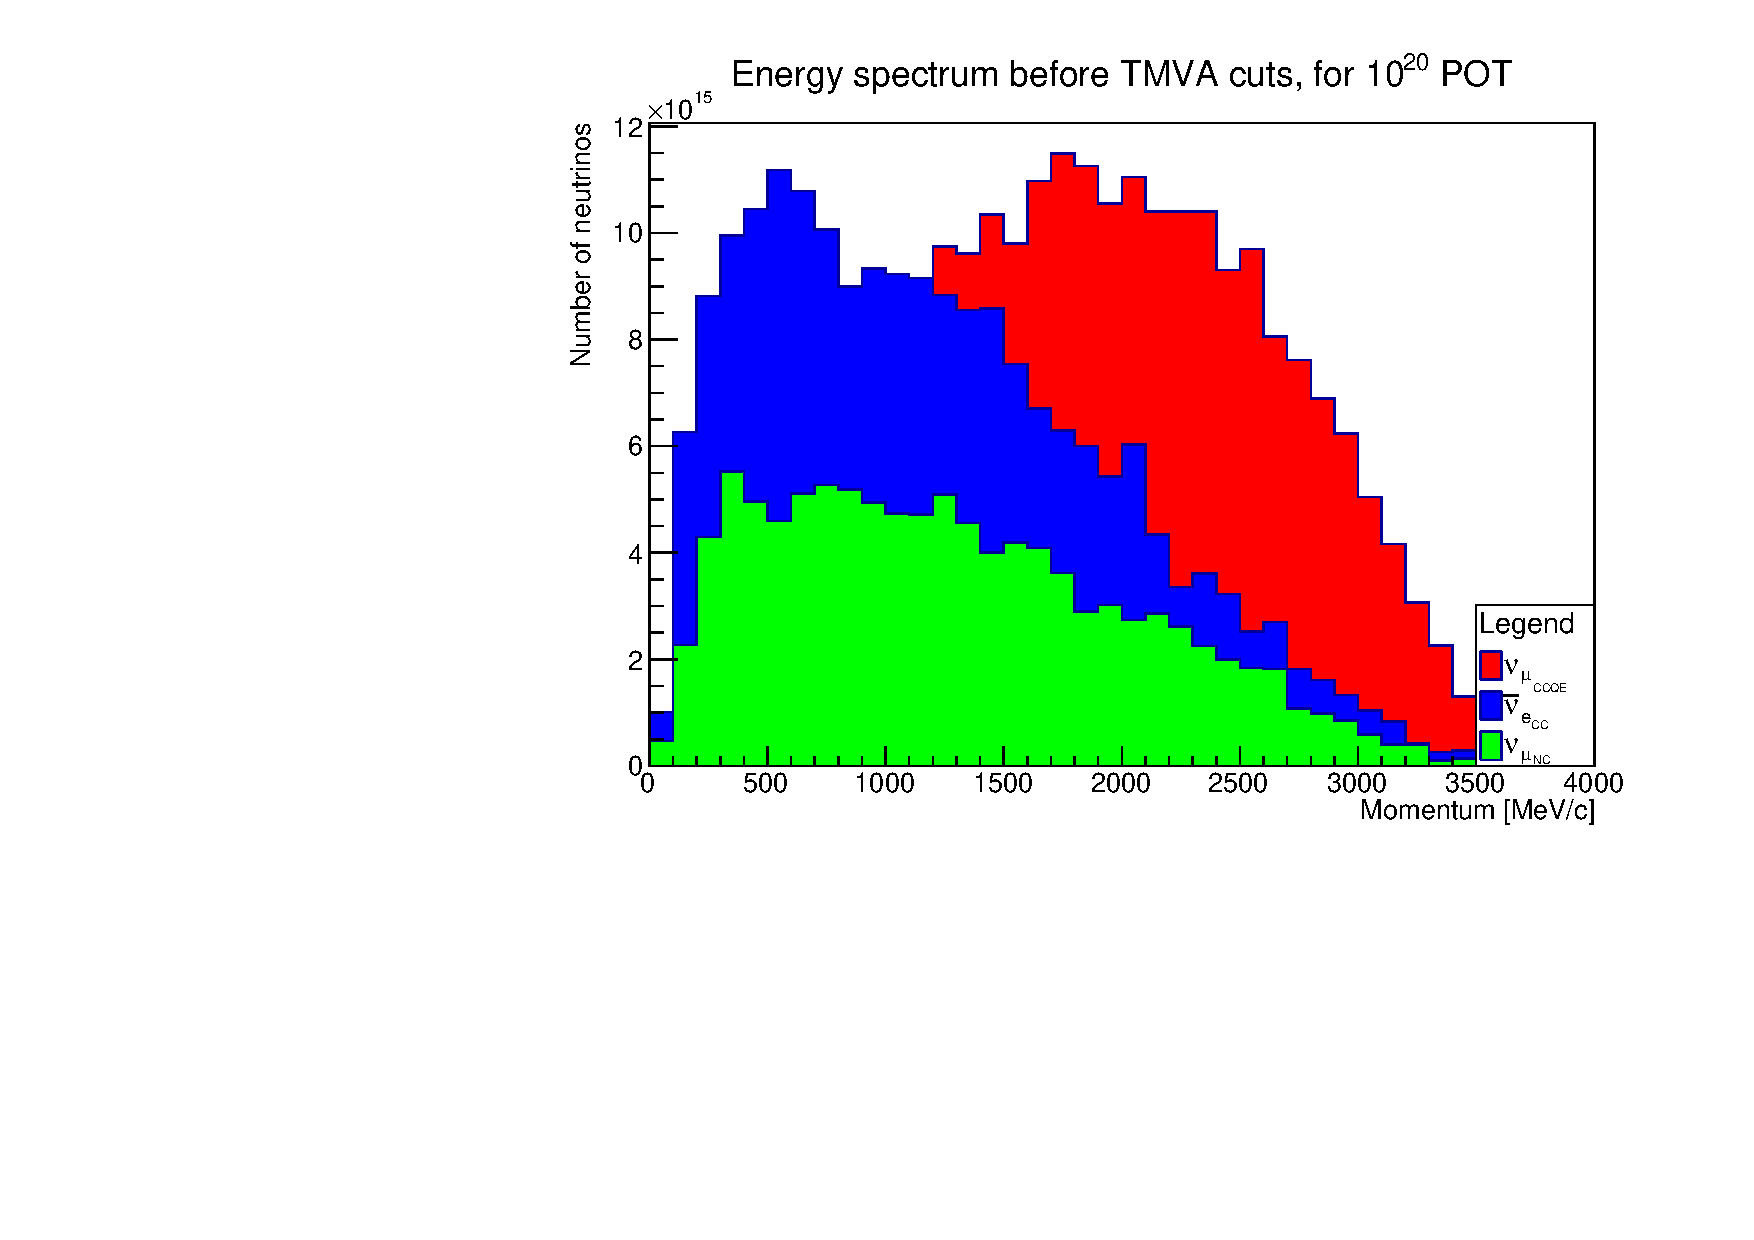
\includegraphics[width=.9\textwidth]{figures/NeutrinoChap/ActualNeutrinoEvents.pdf}
%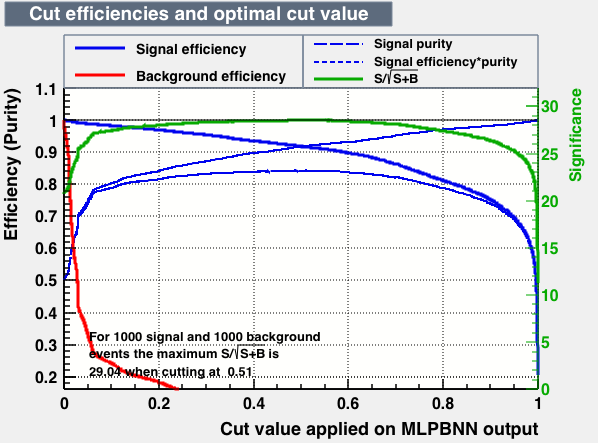
\includegraphics[width=\textwidth]{figures/neutrinoTMVA/mvaeffs_MLPBNN.png}
\caption{Neutrino energy spectrum of $\bar{\nu}_{eCC}$ , $\nu_{\mu_{CC}}$ and $\nu_{\mu_{NC}}$ produced from $10^{20}$ protons-on-target (POT), before passing through the TMVA algorithm.}
\label{fig:TMVAEspectrumBefore}
\end{figure}


\begin{figure}[h!]
\centering
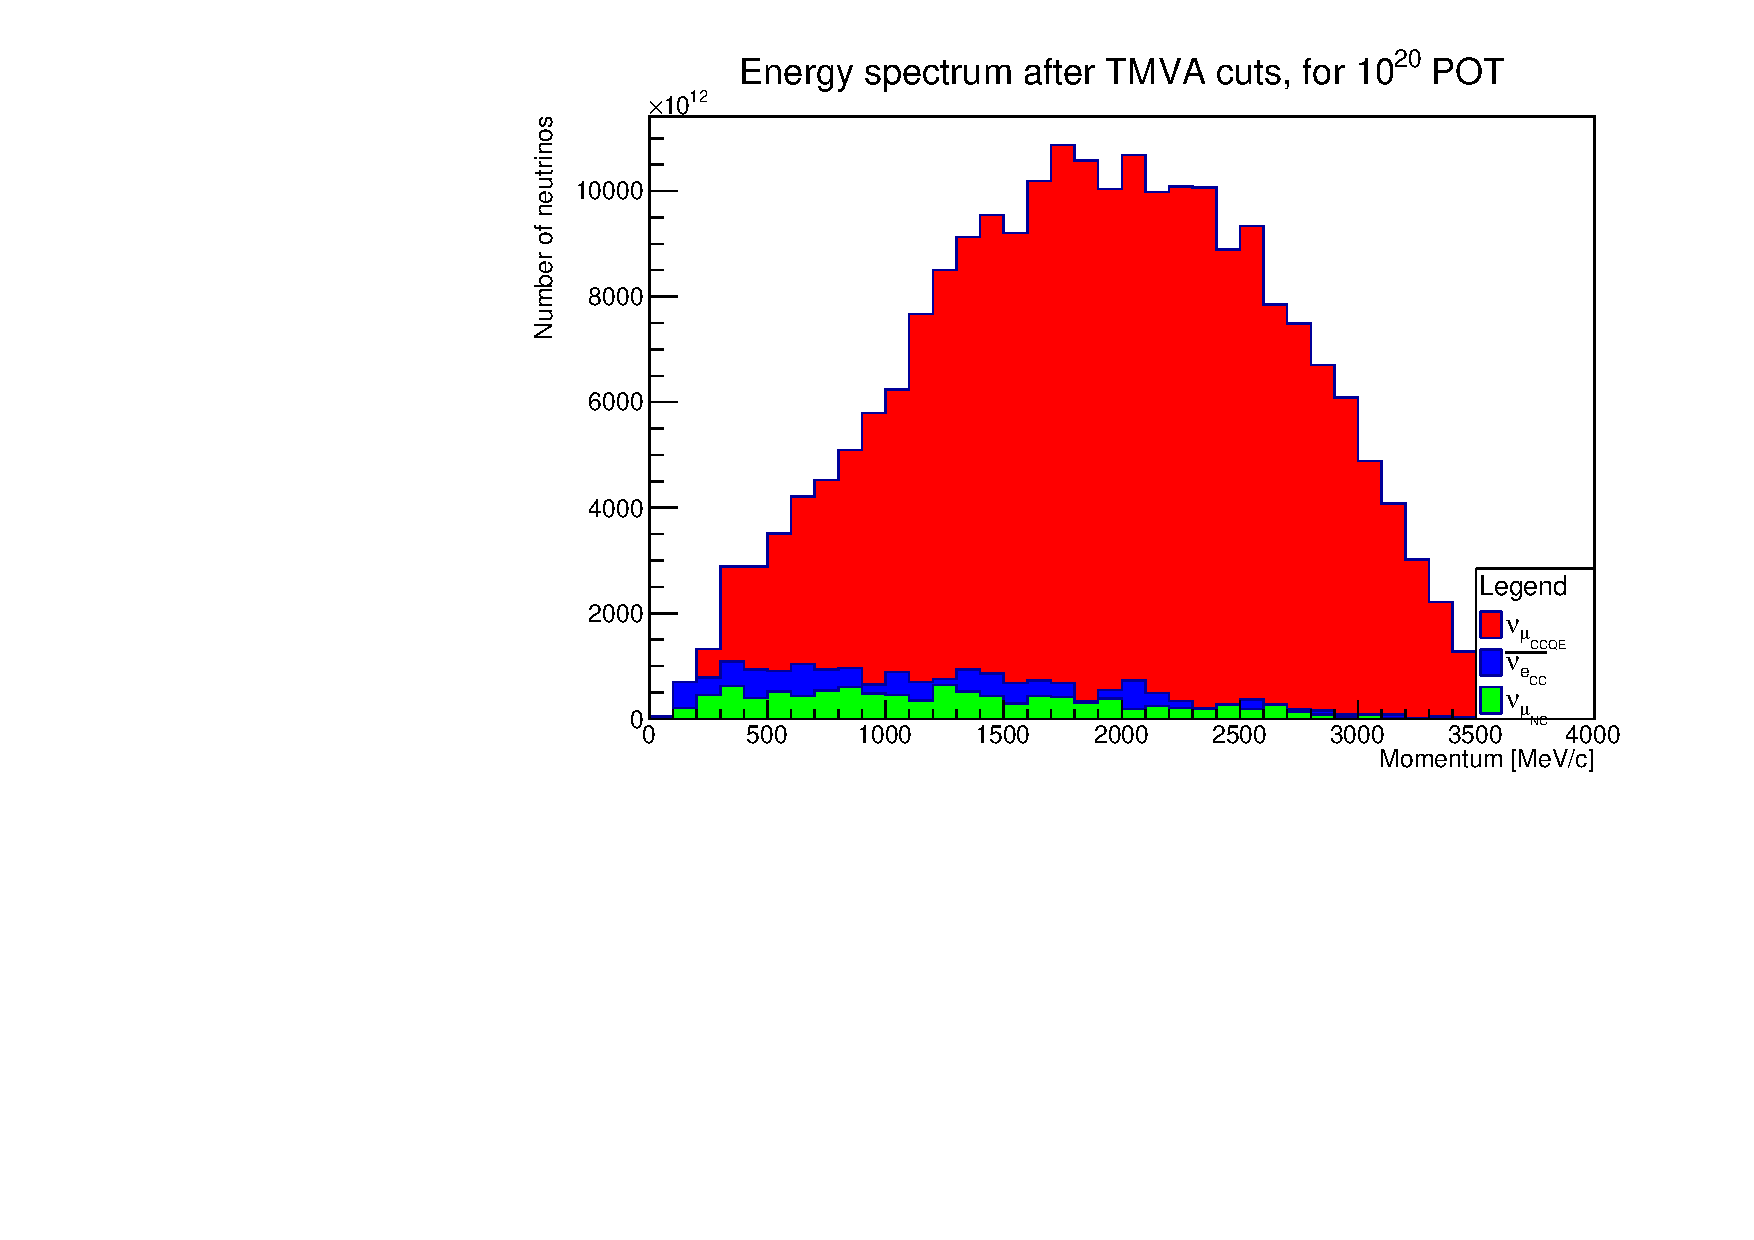
\includegraphics[width=.9\textwidth]{figures/NeutrinoChap/ActualNeutrinoEventsAfter.pdf}
%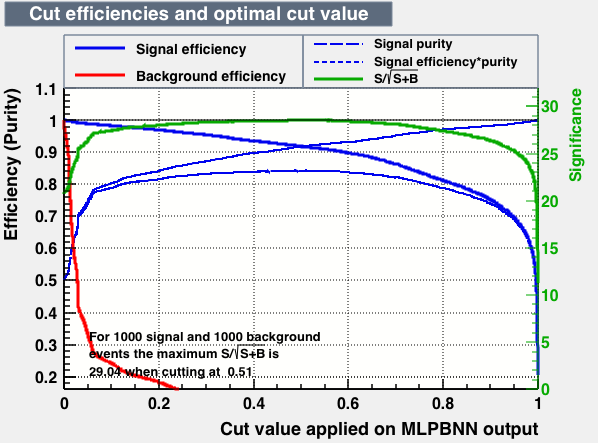
\includegraphics[width=\textwidth]{figures/neutrinoTMVA/mvaeffs_MLPBNN.png}
\caption{Neutrino energy spectrum of $\bar{\nu}_{eCC}$, $\nu_{\mu_{CC}}$and $\nu_{\mu_{NC}}$ produced from $10^{20}$ protons-on-target (POT), after passing through the TMVA algorithm.}
\label{fig:TMVAEspectrumAfter}
\end{figure}

\section{Expected neutrino scattering results at the NuSTORM beam}

Using the tabled event rates for $10^{21}$ protons-on-target (POT) estimated for a 100 ton detector 50 m for the nuSTORM storage ring provided in~\cite{118Soler} the spectra in figures~\ref{fig:TMVAEspectrumBefore} and~\ref{fig:TMVAEspectrumAfter} can be converted to number of events. In NuSTORM the following events are expected: $6.1\times 10^6$ $\nu_\mu$ CC events, $2.5\times 10^6$ $\bar{\nu}_e$ CC events, $2.1\times 10^6$ $\nu_\mu$ NC events and $1.0\times 10^6$ $\bar{\nu}_e$ NC events in a 100 ton detector for $10^{21}$ POT. The numbers used were reduced by a factor of 10 to provide an estimate for a 10 ton detector and the final result can be seen in figures~\ref{fig:TMVAEspectrumNBefore} and~\ref{fig:TMVAEspectrumNAfter}.

\begin{figure}[h!]
\centering
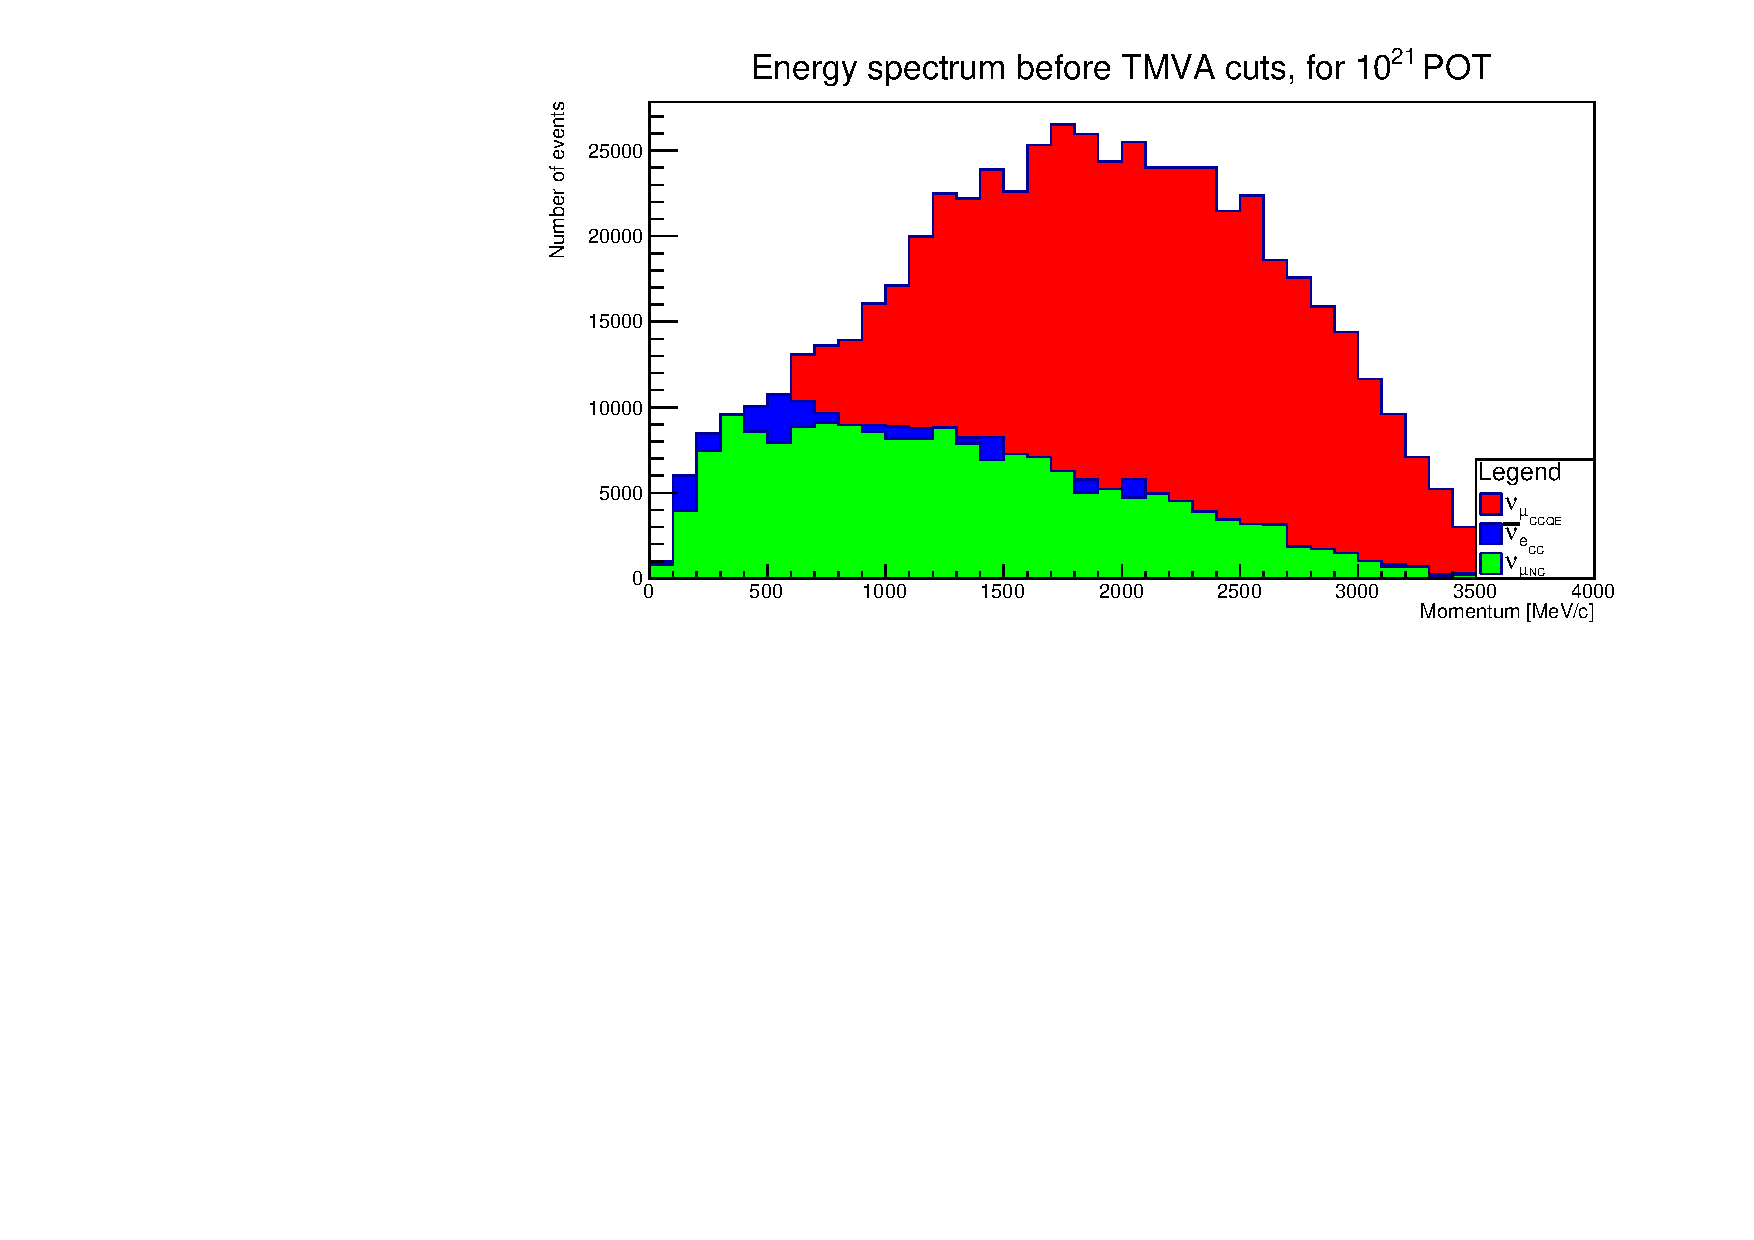
\includegraphics[width=.9\textwidth]{figures/NeutrinoChap/NuSTORM/ActualNumEvents.pdf}
%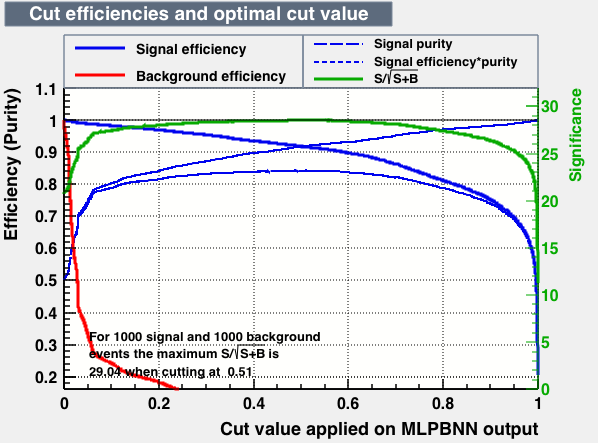
\includegraphics[width=\textwidth]{figures/neutrinoTMVA/mvaeffs_MLPBNN.png}
\caption{Neutrino energy spectrum of $\bar{\nu}_{eCC}$ , $\nu_{\mu_{CC}}$ and $\nu_{\mu_{NC}}$ recorded from $10^{21}$ protons-on-target (POT) in a 10 ton detector at 50 m, before passing through the TMVA algorithm.}
\label{fig:TMVAEspectrumNBefore}
\end{figure}

\begin{figure}[h!]
\centering
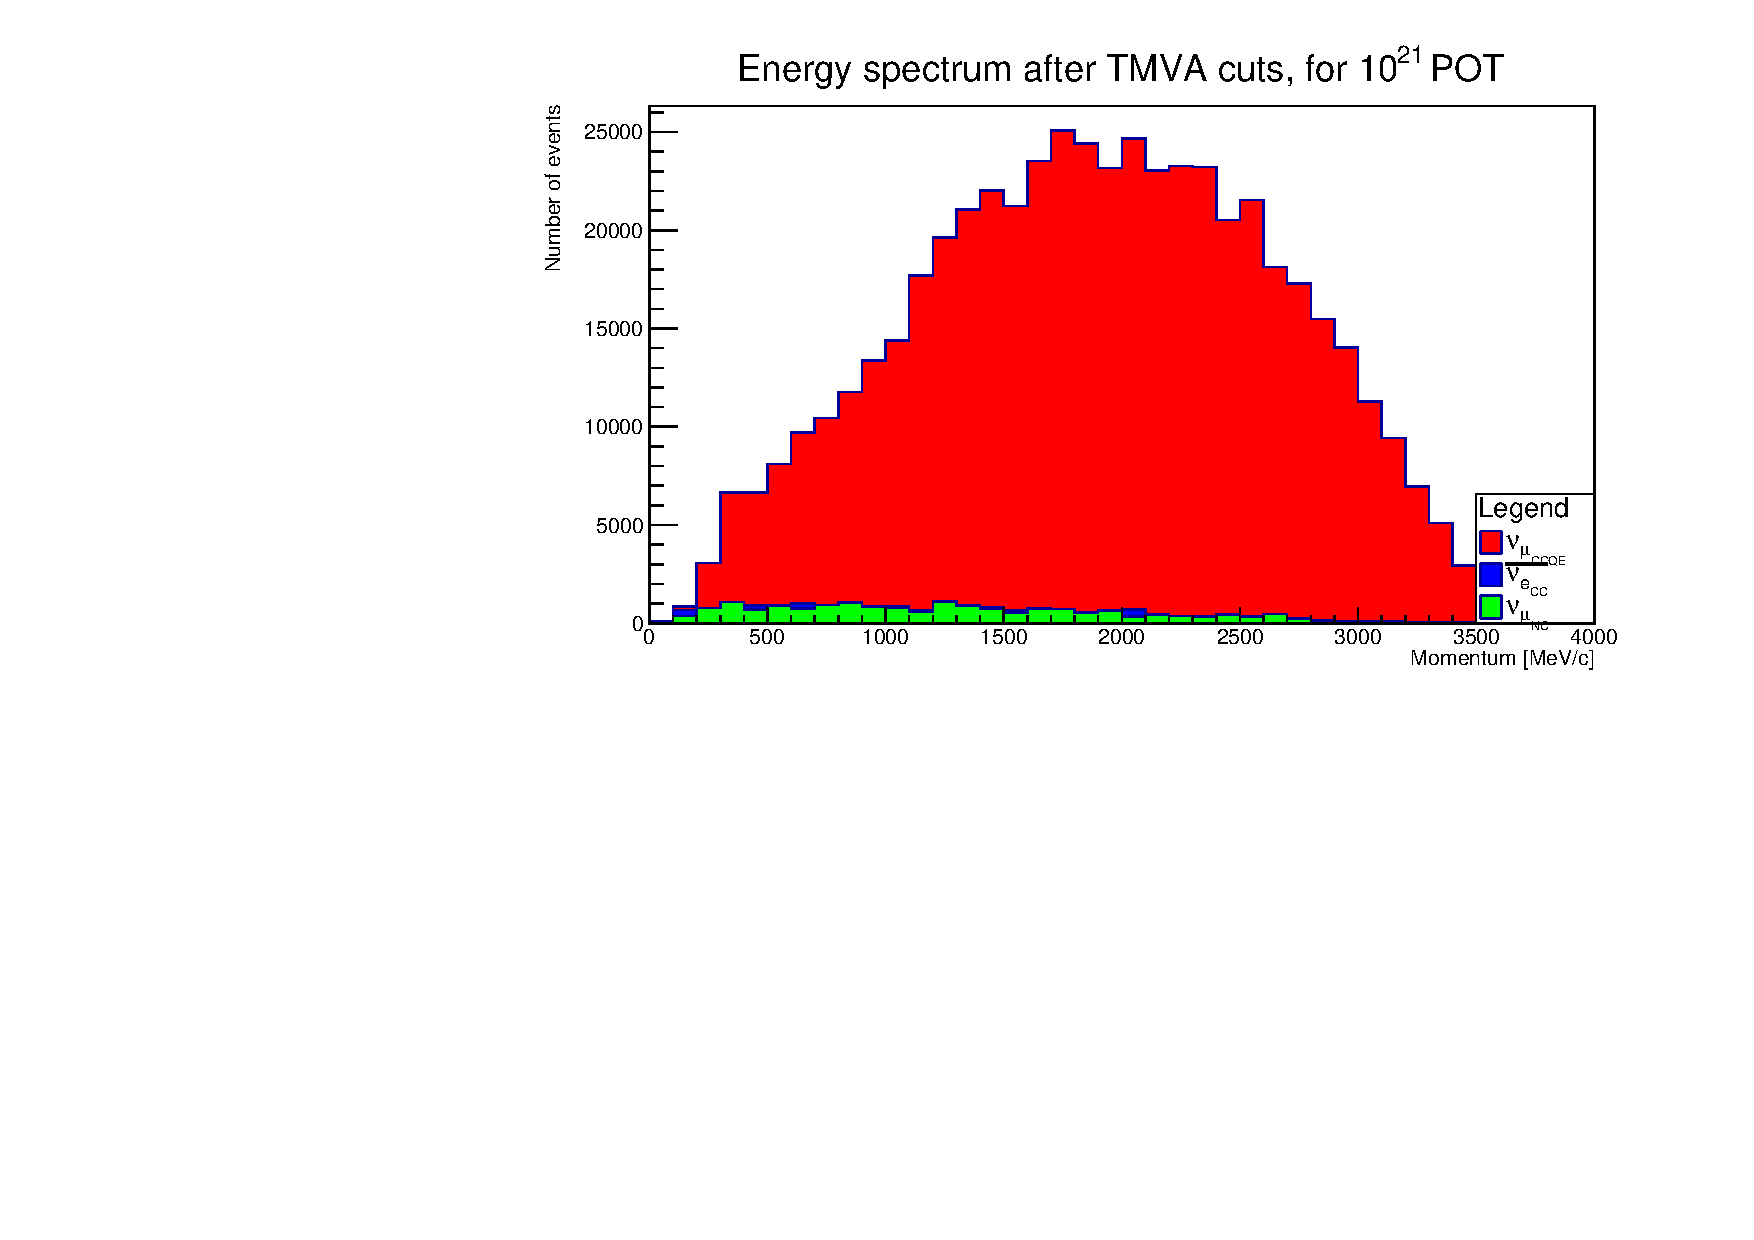
\includegraphics[width=.9\textwidth]{figures/NeutrinoChap/NuSTORM/ActualNumEventsAfterTMVA.pdf}
%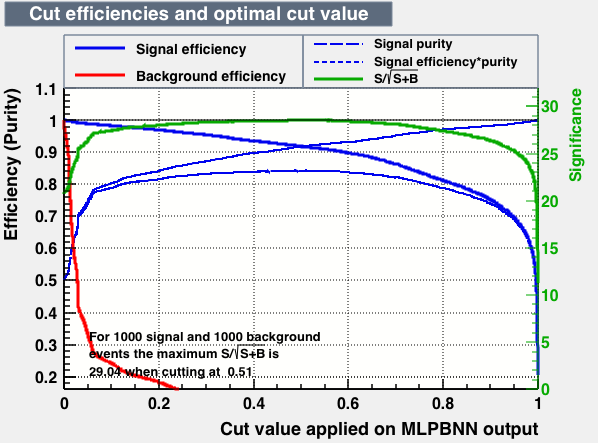
\includegraphics[width=\textwidth]{figures/neutrinoTMVA/mvaeffs_MLPBNN.png}
\caption{Neutrino energy spectrum of $\bar{\nu}_{eCC}$, $\nu_{\mu_{CC}}$and $\nu_{\mu_{NC}}$ recorded from $10^{21}$ protons-on-target (POT) in a 10 ton detector at 50 m, after passing through the TMVA algorithm.}
\label{fig:TMVAEspectrumNAfter}
\end{figure}

The result of the TMVA can be combined to estimate the total statistical and systematic error on the cross-section measurement possible in a NuSTORM beam line. 

\newcommand*\subsetadd{\mathrel{\ooalign{$\bigcup$\cr\hidewidth\hbox{$\oplus\mkern 0.5mu$}\cr}}}

The CC inclusive cross section is given by the subtraction of the total background from the signal, and dividing by the neutrino flux and the total number of nucleons in the detector.  The estimated uncertainty is given by the quadratic sum of the errors for the signal and the total background. By defining the following operation, $a \oplus b = \sqrt{a^2+b^2}$ and generalising it as $\subsetadd x_i \equiv \sqrt{\sum x_i ^2}$, the error is defined through combining each error as $\sigma_{\nu_{\mu CC}} \oplus \sigma_{\bar{\nu}_{eCC}} \oplus \sigma_{\nu_{NC}} $. Using this error estimate combined with the cross-section values from~\FigRef{fig:neutrinoInteractionsFig} results in the determination of the $\nu_\mu$ inclusive CC cross section, as shown in~\FigRef{fig:crossSecEst} with the estimated measurement errors included.

The results show that it is possible to measure the neutrino inclusive CC cross section with small statistical errors (of order 3\% per bin), for a 10 ton detector in the NuSTORM beam at $10^{21}$ POT. These errors would decrease with a larger detector mass as well as with more protons on target.

\begin{figure}[h!]
\centering
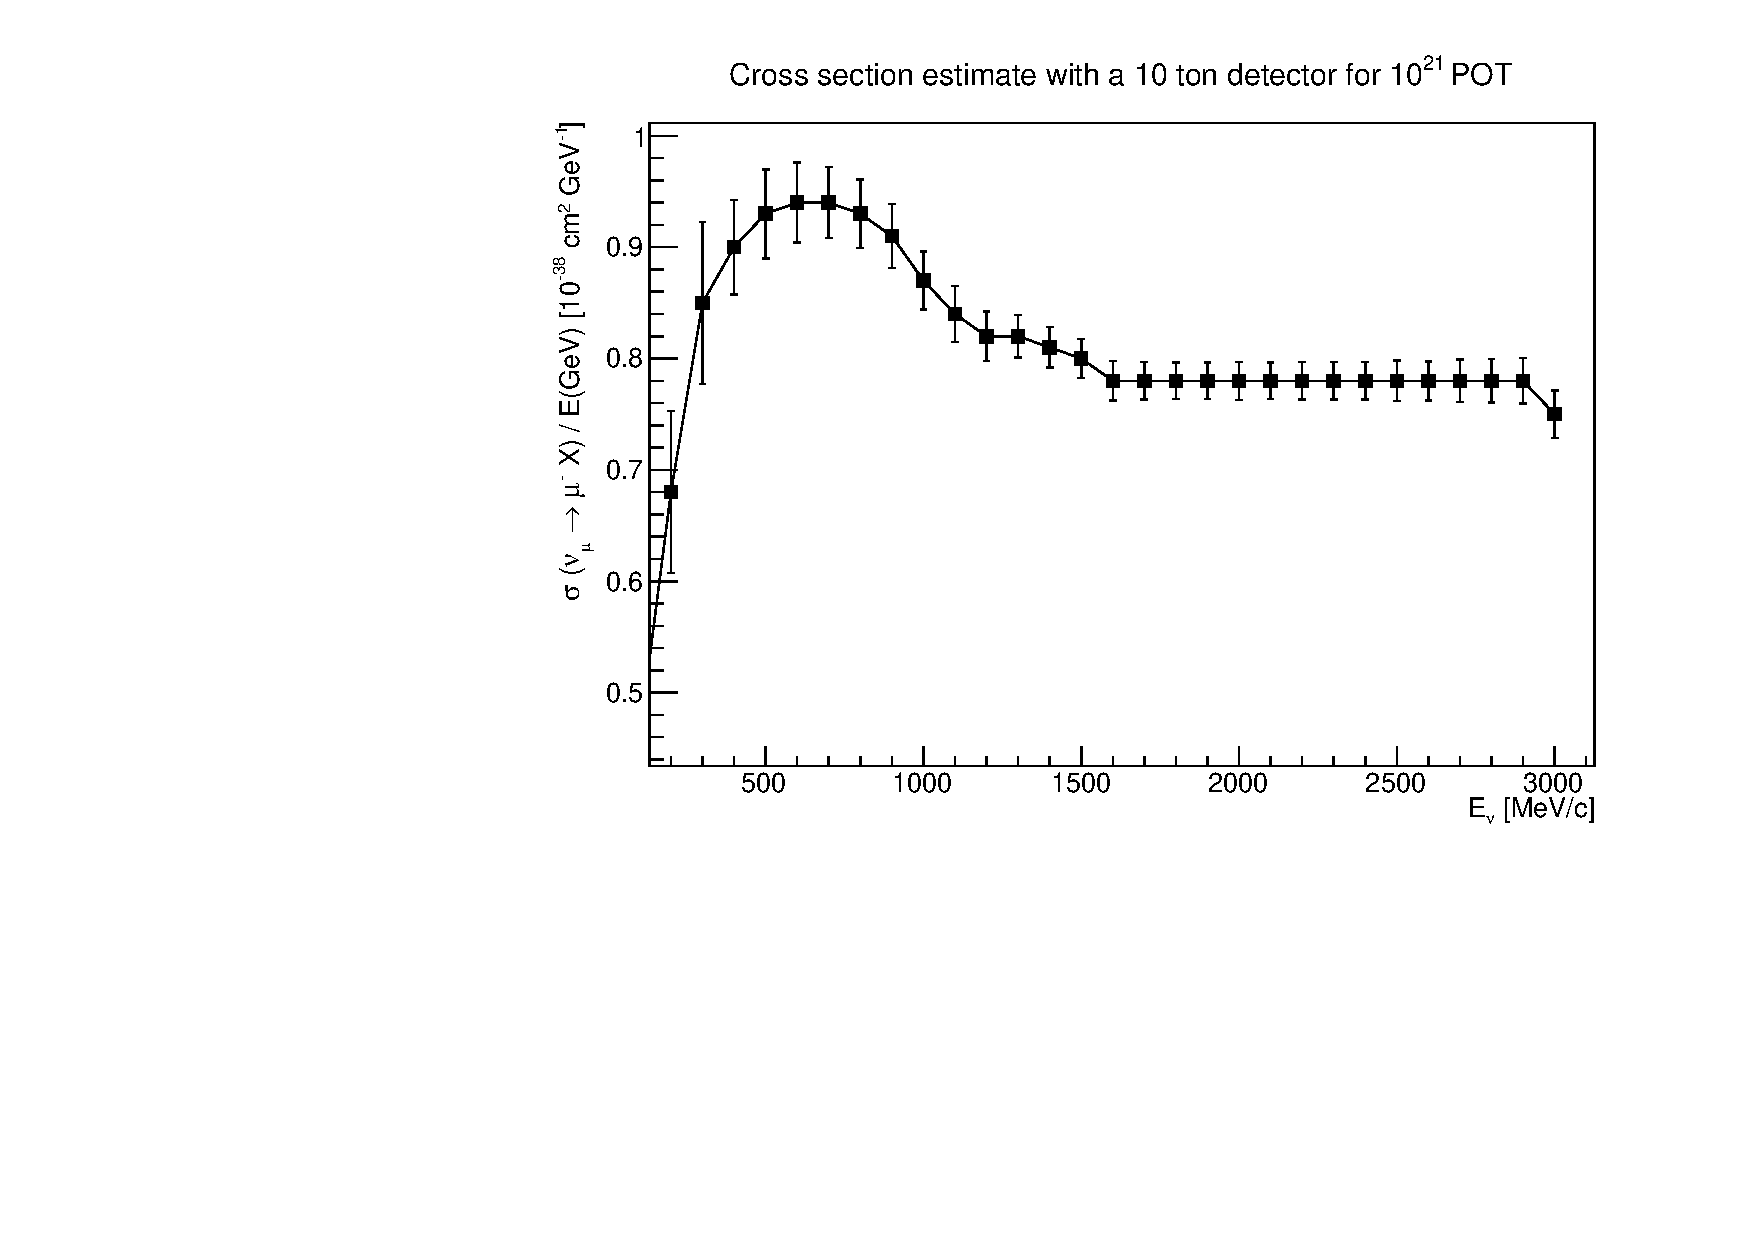
\includegraphics[width=.9\textwidth]{figures/NeutrinoChap/NuSTORM/CrossSecEstimateNew.pdf}
%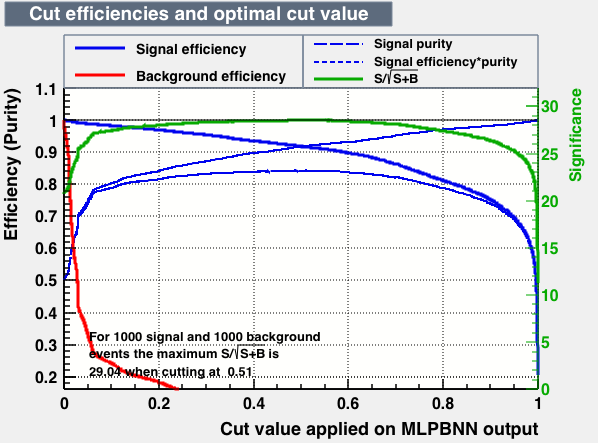
\includegraphics[width=\textwidth]{figures/neutrinoTMVA/mvaeffs_MLPBNN.png}
\caption{Inclusive neutrino CC cross section for a 10 ton detector at a NuSTORM beam with $10^{21}$ POT. The cross section from~\FigRef{fig:neutrinoInteractionsFig} is overlayed with error bars estimated from this study.}

%\caption{Neutrino cross section from ~\FigRef{fig:neutrinoInteractionsFig} overlayed with error bars estimated from the Baby MIND study.}
\label{fig:crossSecEst}
\end{figure}

%This section should include a summary of the number of events expected if this were run in NuStorm, for a 1 tonne target. Use the number of events expected from my talk at Blacksburg and draw a plot of number of events as a function of energy in bins of neutrino energy. This can be used to calculate the statistical and systematic errors in the cross section of CCQE events. This would finish off this study.




%Describe the NuSTORM beam line again, expected energy of neutrinos.
%Interactions in the TASD, what would be the efficiency of identifying mu CCQE events in a background e CC and mu NC ? 
%New MC study using TMVA again, show plots and work. Show training and testing samples. Create mixed sample and show how well it can identify the parts. 

%\pagebreak
%\newpage

\section{Summary}
From the NuSTORM study carried out in this chapter, a detector configuration consisting of a Totally Active Scintillator Detector (TASD) with a Baby MIND spectrometer downstream would be able to provide charge reconstruction of tracks down to 400 GeV/c with the possibility to identify and distinguish between the $\nu_{\mu_{CC}}$ signal in a background of $\bar{\nu}_{eCC}$, $\nu_{\mu NC}$ and $\bar{\nu}_{eNC}$ from the NuSTORM beam with 84\% efficiency and contamination of 7.4\%.



%$\bar{\nu}_{eCC}$ and $\nu_{\mu_{NC}}$ with 84\% efficiency.

%From the NuSTORM study is it clear that a TASD + Baby MIND configuration would be able to provide charge reconstruction of tracks down to 400 GeV/c with the possibility to identify and distinguish between the $\nu_{\mu_{CC}}$ signal in a background of $\bar{\nu_{e_{CC}}}$ and $\nu_{\mu_{NC}}$ with 91.3 \% efficiency.


%\subsection{Interactions in TASD + Baby MIND T2K (Remove?)}
\pagebreak
\newpage
\chapter{J-PARC beam neutrino interaction studies}
\label{c:neutrinoT2K}

%During the construction of Baby MIND, it was proposed to potentially fully instrument the whole TASD, used during the first beam test, and use it as a fully active target to be combined with Baby MIND, illustrated in~\FigRef{fig:TASDandMIND2}.

%\begin{figure}[h!]
%\centering
%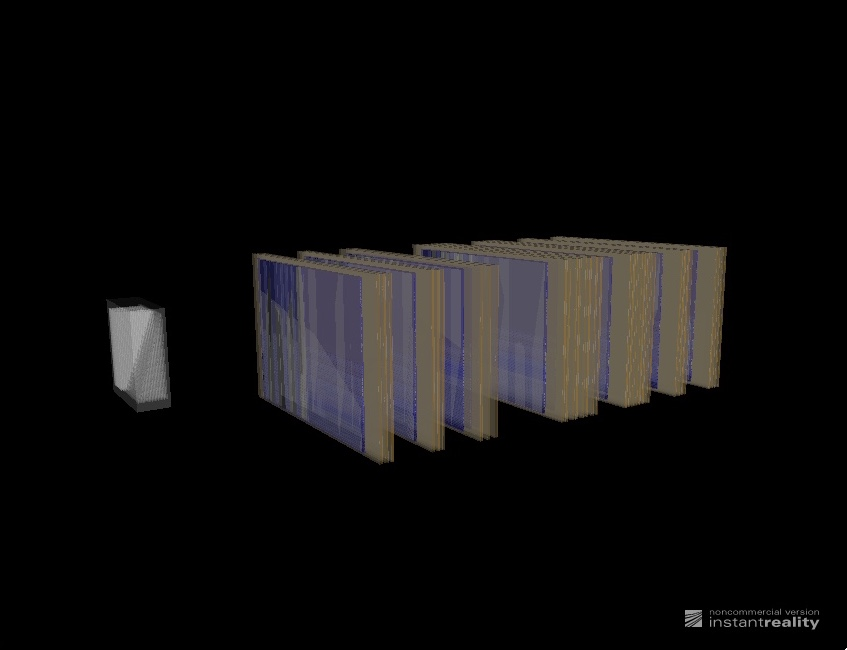
\includegraphics[width=0.9\textwidth]{figures/MINDAida.jpeg}
%\caption{An illustrative sketch of the detector setup with the TASD detector in front of Baby MIND.}
%\label{fig:TASDandMIND2}
%\end{figure}

%\subsection{Interactions in TASD + Baby MIND}

%For all analysis the TASD is used as a CCQE identification and neutrino veto, expecting two tracks (neutrino) or atleast start of muon track. The dimensions are the same as mentioned under the test beam section, with a distance of 368mm between the two detectors. Neutrinos are simulated using the T2K near detector spectrum in reverse horn current mode (RHC), seen in~\FigRef{fig:T2KndSpectrum} in the SAURON framework. 

%Dont actually have the plots?

%Reshow the muon beam? Discussion about angle etc...

%Have simulations both for T2K and NuSTORM beamline, describe both.
%Full analysis in MIND, only TASD as veto.
 %Shown at NuSTORM talk, fix momentum slightly.
 
%\FloatBarrier
%\pagebreak
%\newpage
\section{Neutrino interactions in iron in Baby MIND}

Neutrinos at T2K are produced from a 30 GeV/c proton beam impinging on a graphite target with three horns to focus the correct polarity of pions that decay to produce neutrinos with the flux spectrum, given by reference~\cite{119T2K}. The INGRID on-axis detector \cite{120INGRID}, performs measurements of the beam direction and on-axis flux.The ND280 experiment uses the beam at a $2.5^\circ$ off-axis angle at a distance of 280 m which provides a narrower energy spectrum with a shifted energy peak at 600 MeV, as can be seen in \FigRef{fig:T2KAxis}. The energy spectrum at the $1.5^\circ$ off-axis angle for the WAGASCI detector has a peak at a higher energy, 800 MeV, than the peak from the $2.5^\circ$ off-axis angle of the ND280 detector, as can be seen in~\FigRef{fig:T2KAxis2}. 


%The WAGASCI $1.5^\circ$ off-axis energy spectrum is shifted at a slightly higher energy than the $2.5^\circ$ off-axis energy spectrum used for the ND280 experiment.

%previous narrower and lower peak than on-axis and slightly higher energy than 2.0 and 2.5 deg. as seen in plots from NuFact talk. Beam comes with two modes, forward horn current (FHC) with neutrinos produced and reverse horn current with anti-neutrinos produced.

\begin{figure}[h!]
\centering
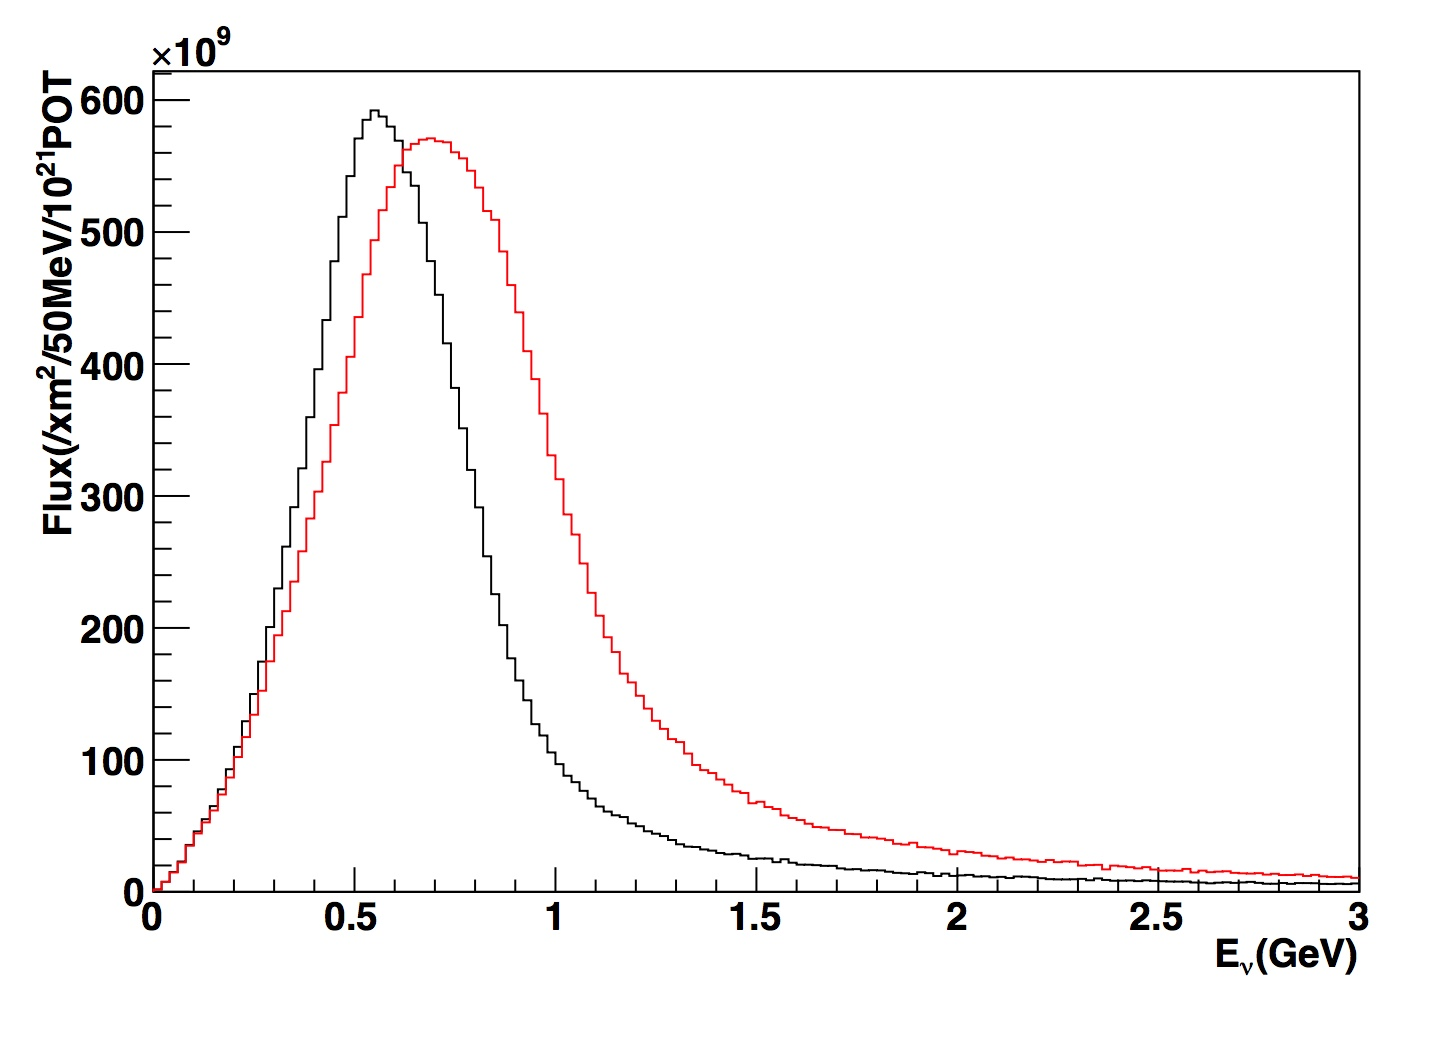
\includegraphics[width=0.9\textwidth]{figures/NeutrinoChap/ND280vsWAGASCIspectrum.jpeg}
\caption{Neutrino energy spectrum for WAGASCI (red, off-axis $1.5^\circ$) and ND280 (black, off-axis $2.5^\circ$). The peak energy at $1.5^\circ$ degrees is 800 MeV, with respect to the peak energy of 600 MeV at $2.5^\circ$. Figure, courtesy of Akihiro Minamino.}
\label{fig:T2KAxis}
\end{figure}

\begin{figure}[h!]
\centering
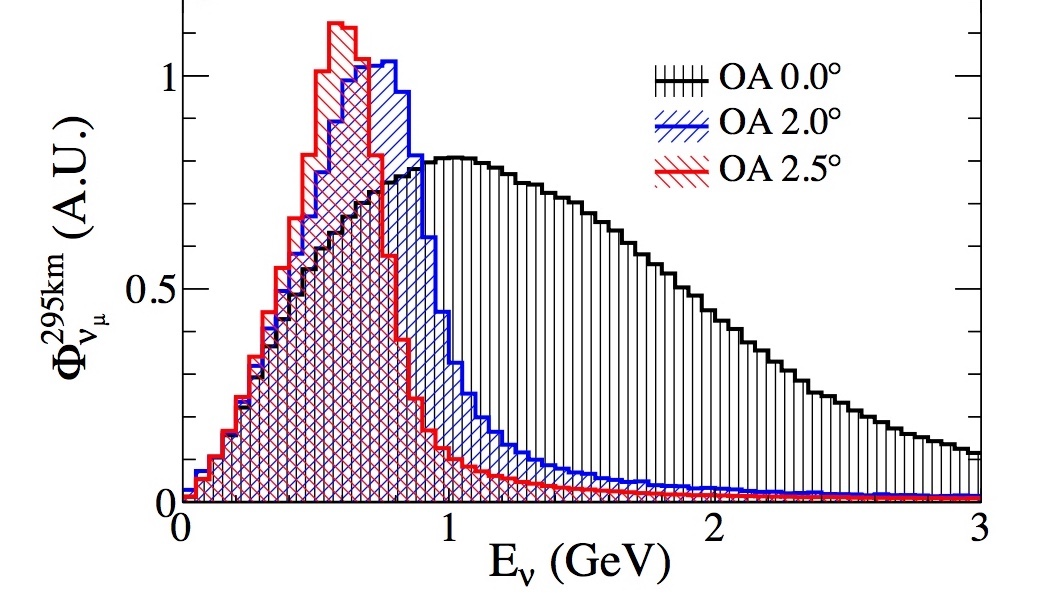
\includegraphics[width=0.9\textwidth]{figures/NeutrinoChap/offAxisFlux.jpeg}
\caption{Neutrino energy spectrum of the J-PARC neutrino beam extrapolated to 295 km for various off-axis angles in degrees. Figure, courtesy of Akihiro Minamino.}
\label{fig:T2KAxis2}
\end{figure}

%You have to introduce what you are going to do in this chapter and give some context. You can’t assume that the reader knows the conditions for data taking or why you are doing this. 

%Explain that the goal of this chapter is to measure for the first time neutrino interactions in the iron of Baby MIND. Explain also that the data was taken during the commissioning of Baby MIND at J-PARC between March and May 2018. You need to also explain that the beam was operated in reverse horn current since it is important to realise that there is a larger contamination of neutrinos in the predominantly antineutrino beam. Please add a few paragraphs here to introduce all of this before you start talking about your simulation etc.

The goal of this chapter is to perform the first measurement of neutrino interactions in the iron of Baby MIND. To validate the simulation framework SAURON, simulations will be compared to the recorded data. Data for the study were taken during the commissioning of Baby MIND at J-PARC between March and May 2018 when the beam was operated in reverse horn current mode. This mode produces a majority of muon antineutrinos with a contamination of muon neutrinos.

The reverse horn current neutrino and antineutrino spectrum at 1.5$^\circ$ that the WAGASCI and Baby MIND detectors observed in the run between March and May 2018 can be seen in \FigRef{fig:T2KndSpectrum}. The fraction of muon antineutrinos is approximately 92\%, with a mean energy of 1.43 GeV, and the fraction of muon neutrinos is approximately 9\%, with a mean energy of 0.86 GeV. These spectra were used to perform simulations of neutrino and antineutrino events in WAGASCI and Baby MIND.

%For the simulations the WAGASCI spectrum has been used, and the combined spectrum of muon neutrinos and antineutrinos for reverse horn current can be seen in \FigRef{fig:T2KndSpectrum}. In this mode the fraction of muon neutrinos is approximately $8\%$ with a mean energy of $0.86$ GeV/c and muon antineutrinos of muon neutrinos is approximately $92\%$ with a mean energy of $1.43$ GeV/c.


%The reverse horn current neutrino and antineutrino spectrum at 1.5$^\circ$ that the WAGASCI and Baby MIND detectors observed in the run between March and May 2018 can be seen in \FigRef{fig:T2KndSpectrum}. The fraction of muon antineutrinos is approximately 92\%, with a mean energy of 1.43 GeV, and the fraction of muon neutrinos is approximately 9\%, with a mean energy of 0.86 GeV. These spectra were used to perform simulations of neutrino and antineutrino events in WAGASCI and Baby MIND.

%In the framework several figures of merit are produced, the muon energy spectrum, reconstructed muon energy spectrum, reconstructability of tracks vs energy and charge reconstruction vs energy. All of these figures of merit are shown in~\FigRef{fig:T2KTASDfitted} and~\FigRef{fig:T2KTASDfittedcharge}. In \FigRef{fig:T2KTASDfittedcharge} the efficiency does not start at 0 as the few tracks which have been fitted can provide a charge, however comparing this with the fitted it is clear this is a minority of tracks seen in \FigRef{fig:T2KTASDCombined} and \FigRef{fig:T2KTASDCombinedZoom}.

\begin{figure}[h!]
\centering
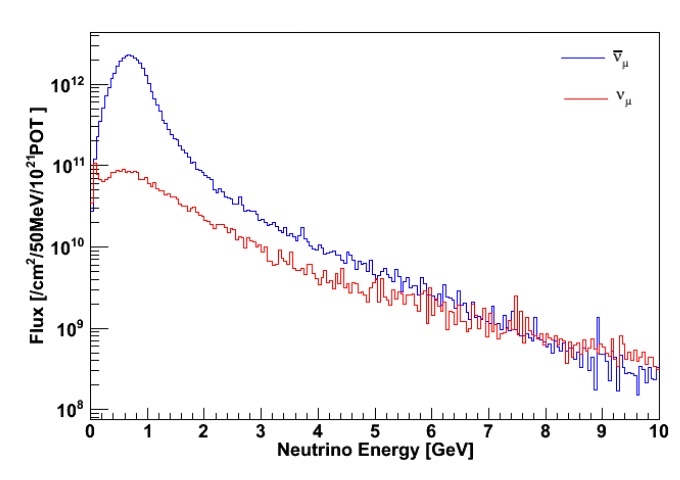
\includegraphics[width=0.9\textwidth]{figures/WAGASCIflux.jpeg}
\caption{The energy spectrum for muon neutrinos and muon antineutrinos in the T2K near detector reverse horn current (RHC) beam. Figure, courtesy of Akihiro Minamino.}
\label{fig:T2KndSpectrum}
\end{figure}

%Similarly to the simulated muon beam, and data the charge reconstruction efficiency is very good for the reconstructible tracks. The difference comes from the fact that the neutrinos are produced at angles instead of straight on the center of the detector (with some beam size). Muons from neutrinos are produced at all angles depending on the kinematics of the neutrino interaction and neutrino energy. 
%Simulations for a  T2K like beam, explain the details and event selection, (None for simulation but easy enough with data). Use the specific fiducial volume. Set up at J-PARC, all the details with that.
%Lead into expected momentum reconstruction? Potential for tracks to be miss constrocted given angle etc etc. Even with cuts on no hit in first plate and hits after iron possible for sand muons to pass through. Tracks leaving would affect reconstruction. Angle and leaving, other than that is should be ok. Few events in total... Number of events sent to Paul, seems resonable.

To compare simulations with data taken for the commissioning run, interactions were simulated in the iron of Baby MIND to perform a standalone Baby MIND analysis, independent of the data taken by the WAGASCI  detector. The fiducial volume selected includes the first three iron plates in the upstream section of Baby MIND (denoted as a1-3 in~\FigRef{fig:MINDneutrinoLayout}) and can be seen in detail in~\FigRef{fig:MINDFiducial}. The selected area is $1 \times 1$ m$^2$ around the centre of the Baby MIND detector providing a total weight of 1500 kg of iron and $9.03 \times 10^{29}$ iron nucleons.

%New paragraph:
%At this point, you define the event selection criteria, ie. the trigger condition of how you choose that a neutrino event is selected.
The event selection has been chosen try to ensure that only muons from neutrino interactions in the iron are evaluated. Firstly to remove outside muons the first veto cut is that there are no hits in the first scintillator module. Secondly to compare to simulations and to reduce muons entering from the side of the detector, at least one hit in each of scintillator module 2, 3 and 4 is required.


%The fiducial volume is chosen to be in the first iron module seen in \FigRef{fig:MINDneutrinoLayout} as a1-3 as well as selecting part of the iron plate, as seen with further details in \FigRef{fig:MINDFiducial}. 

\begin{figure}
\centering
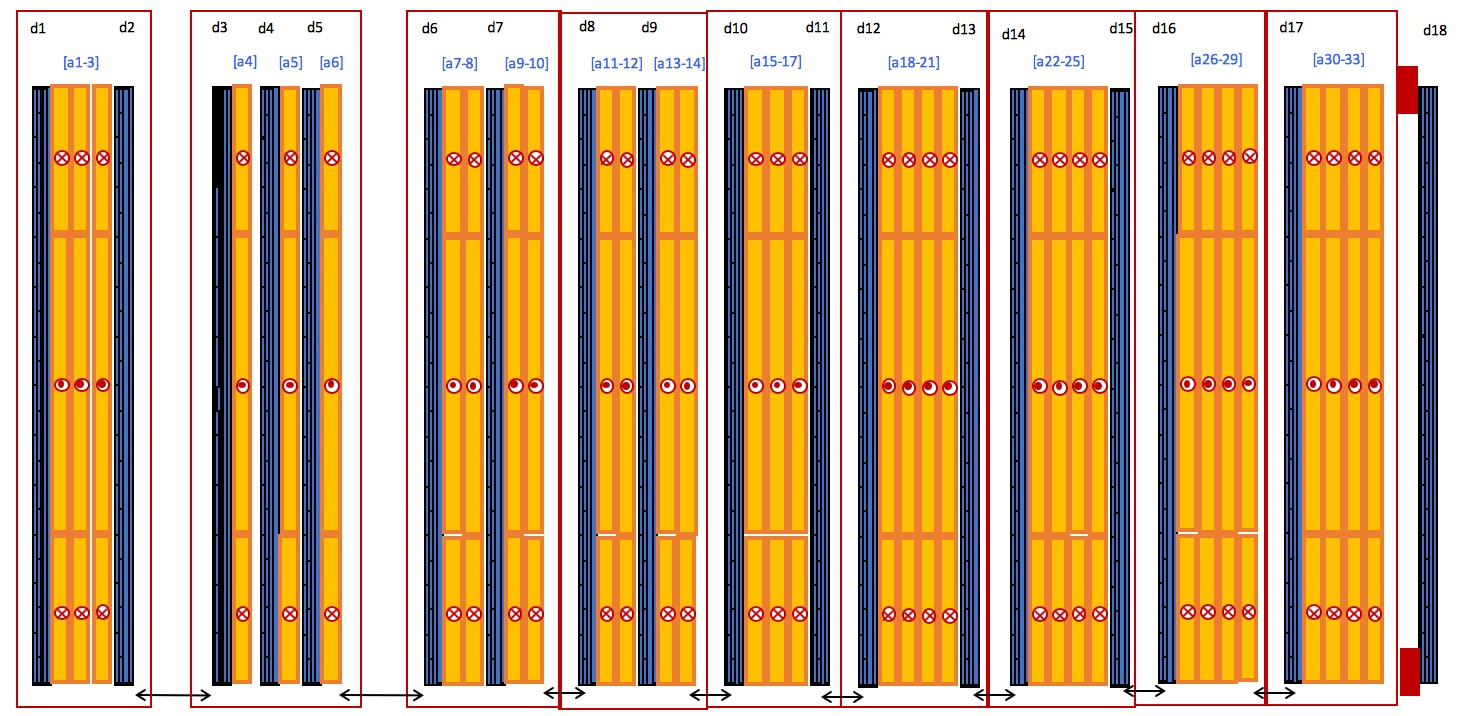
\includegraphics[width=\textwidth]{figures/NeutrinoChap/NuFactTalk/Layout300118.jpeg}
\caption{The layout of the MIND for the commissioning neutrino run.}
\label{fig:MINDneutrinoLayout}
\end{figure}

\begin{figure}
\centering
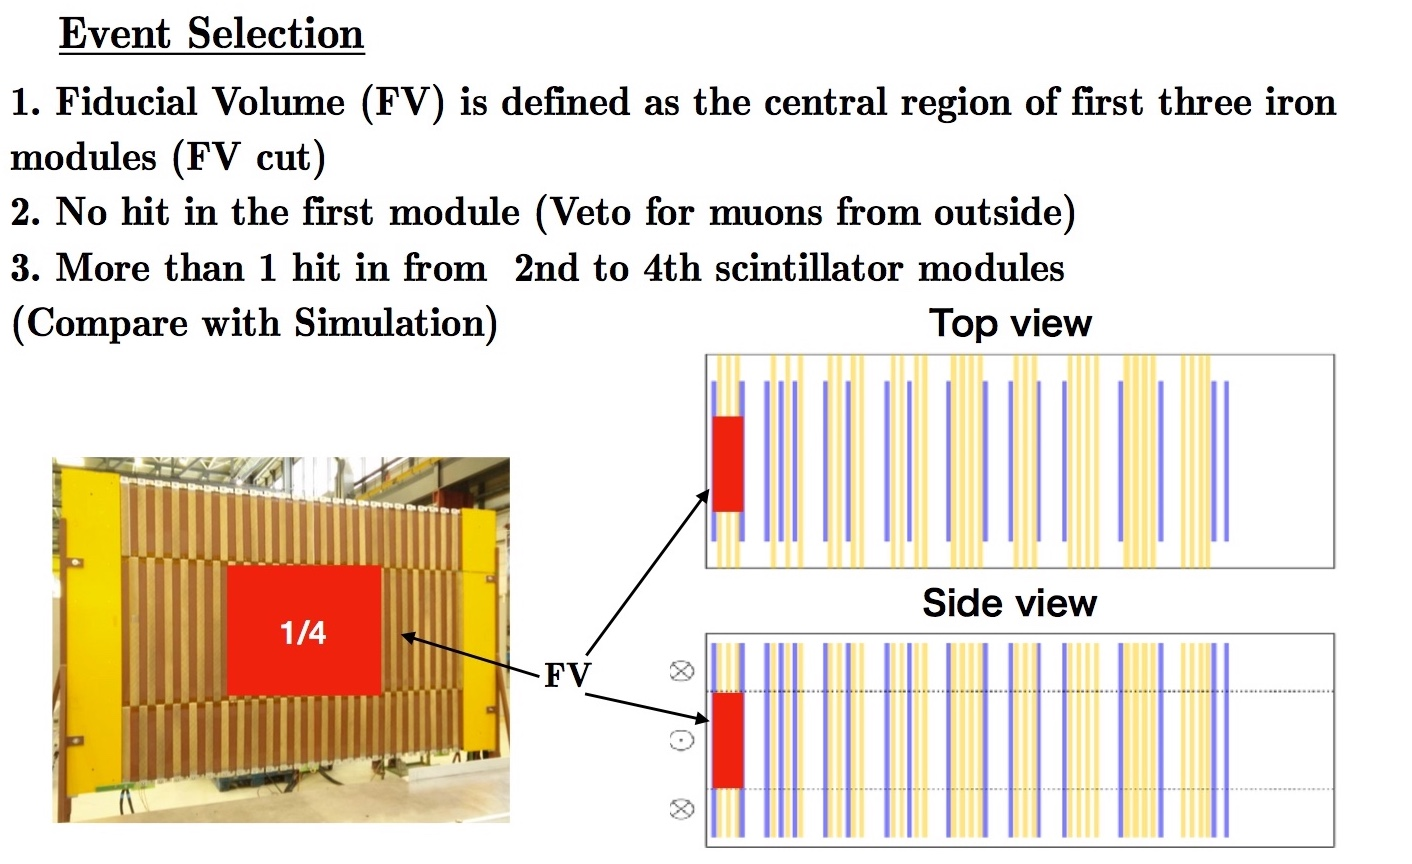
\includegraphics[width=\textwidth]{figures/NeutrinoChap/NuFactTalk/eventRateCheck.jpeg}
\caption{Fiducial volume chosen to measure neutrino events in the first module of iron in the Baby MIND detector. Figure, courtesy of Kenji Yasutome.}
\label{fig:MINDFiducial}
\end{figure}

\section{Reconstruction efficiency of neutrino events in Baby MIND}

%Here you need to describe how you extract the reconstruction efficiency using the simulation, what simulation you used (SAURON or SaRoMaN?), how you generated the events

For the simulations the WAGASCI spectrum has been used in the SAURON framework to generate neutrino interactions in the iron, using event selection previously described. These simulated neutrino events were reconstructed in a similar manner to the interactions in the TASD, detailed in chapter~\ref{c:neutrinoNuSTORM}. The reconstruction efficiency is defined as the ratio of reconstructible tracks divided by all the simulated tracks. The charge efficiency is defined as the number of tracks with the correct charge divided by the number of reconstructible tracks. Multiplying these two results gives the ratio of reconstructed tracks with the correct charge divided by all simulated tracks.

Similarly to the studies carried out in chapter 5 for single muons in the CERN test beam, the charge reconstruction efficiency of muons from neutrino charge current interactions, using the J-PARC neutrino beam, is very high, even at low momenta. The track reconstruction efficiency is shown in~\FigRef{fig:IronMINDfitted} and the charge reconstruction efficiency with respect to the reconstructed track is shown in~\FigRef{fig:IronMINDfittedcharge}.

%The main difference arises from the fact that the neutrinos are produced at a variety of angles with respect to the neutrino direction instead of straight on the center of the detector (with some beam size). Muons from neutrinos are produced at different angles depending on the kinematics of the neutrino interaction and neutrino energy.

In \FigRef{fig:IronMINDfittedcharge} the efficiency for antineutrinos at the lowest momentum does not reach zero as the few tracks which have been fitted can provide a charge. This is seen when multiplying the two plots together as in \FigRef{fig:IronMINDCombined} with a focus on the low momentum range in \FigRef{fig:IronMINDCombinedZoom}.

%In the framework several figures of merit are produced, the muon energy spectrum, reconstructed muon energy spectrum, reconstructability of tracks vs energy and charge reconstruction vs energy. 


% however comparing this with the fitted it is clear this is a minority of tracks seen in \FigRef{fig:T2KTASDCombined}.

\begin{figure}[h!]
\centering
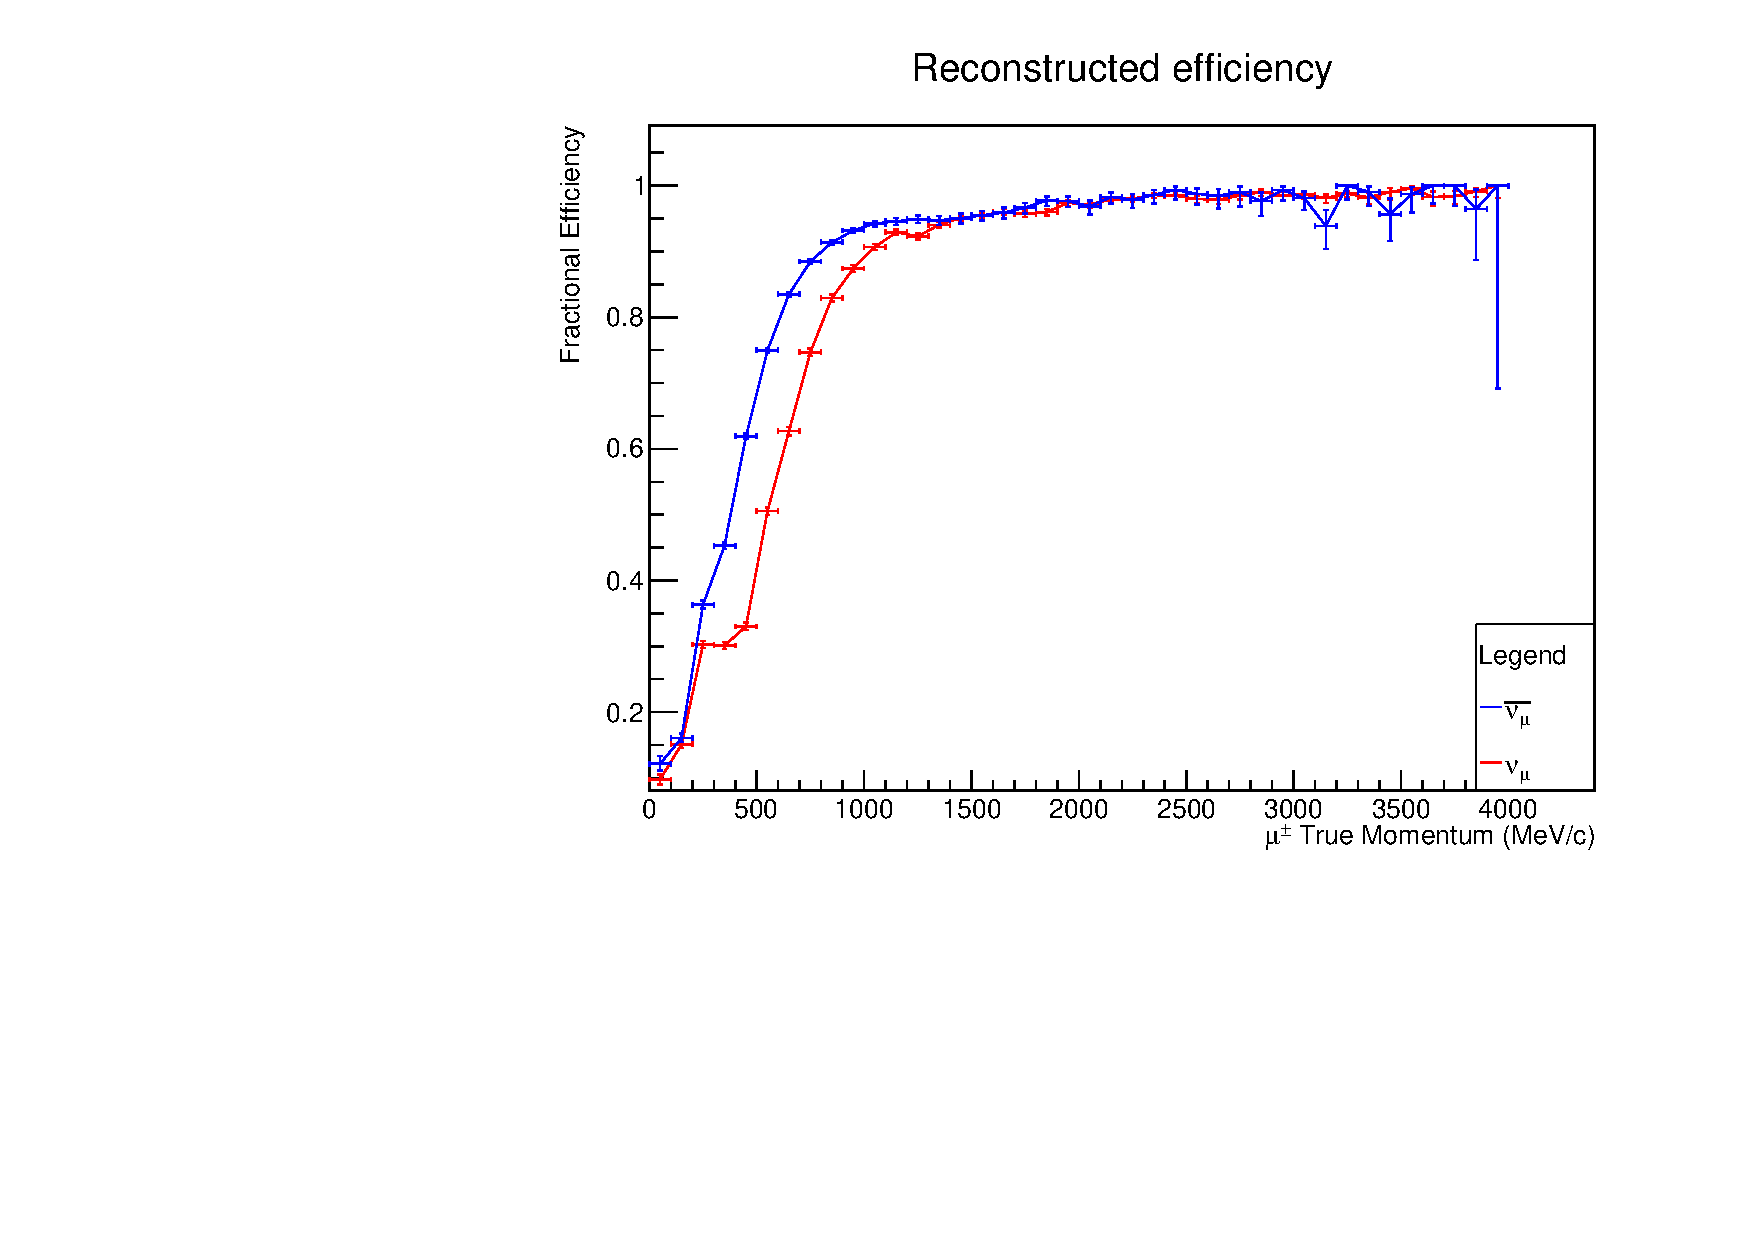
\includegraphics[width=.9\textwidth]{figures/NeutrinoChap/Neutrino/T2KIronRecEff.pdf}
\caption{Track reconstruction efficiency, showing the probability of reconstructing a simulated neutrino charge current event in the first three modules of iron of Baby MIND as a function of the momentum of the reconstructed muon.}
\label{fig:IronMINDfitted}
\end{figure}

\begin{figure}[h!]
\centering
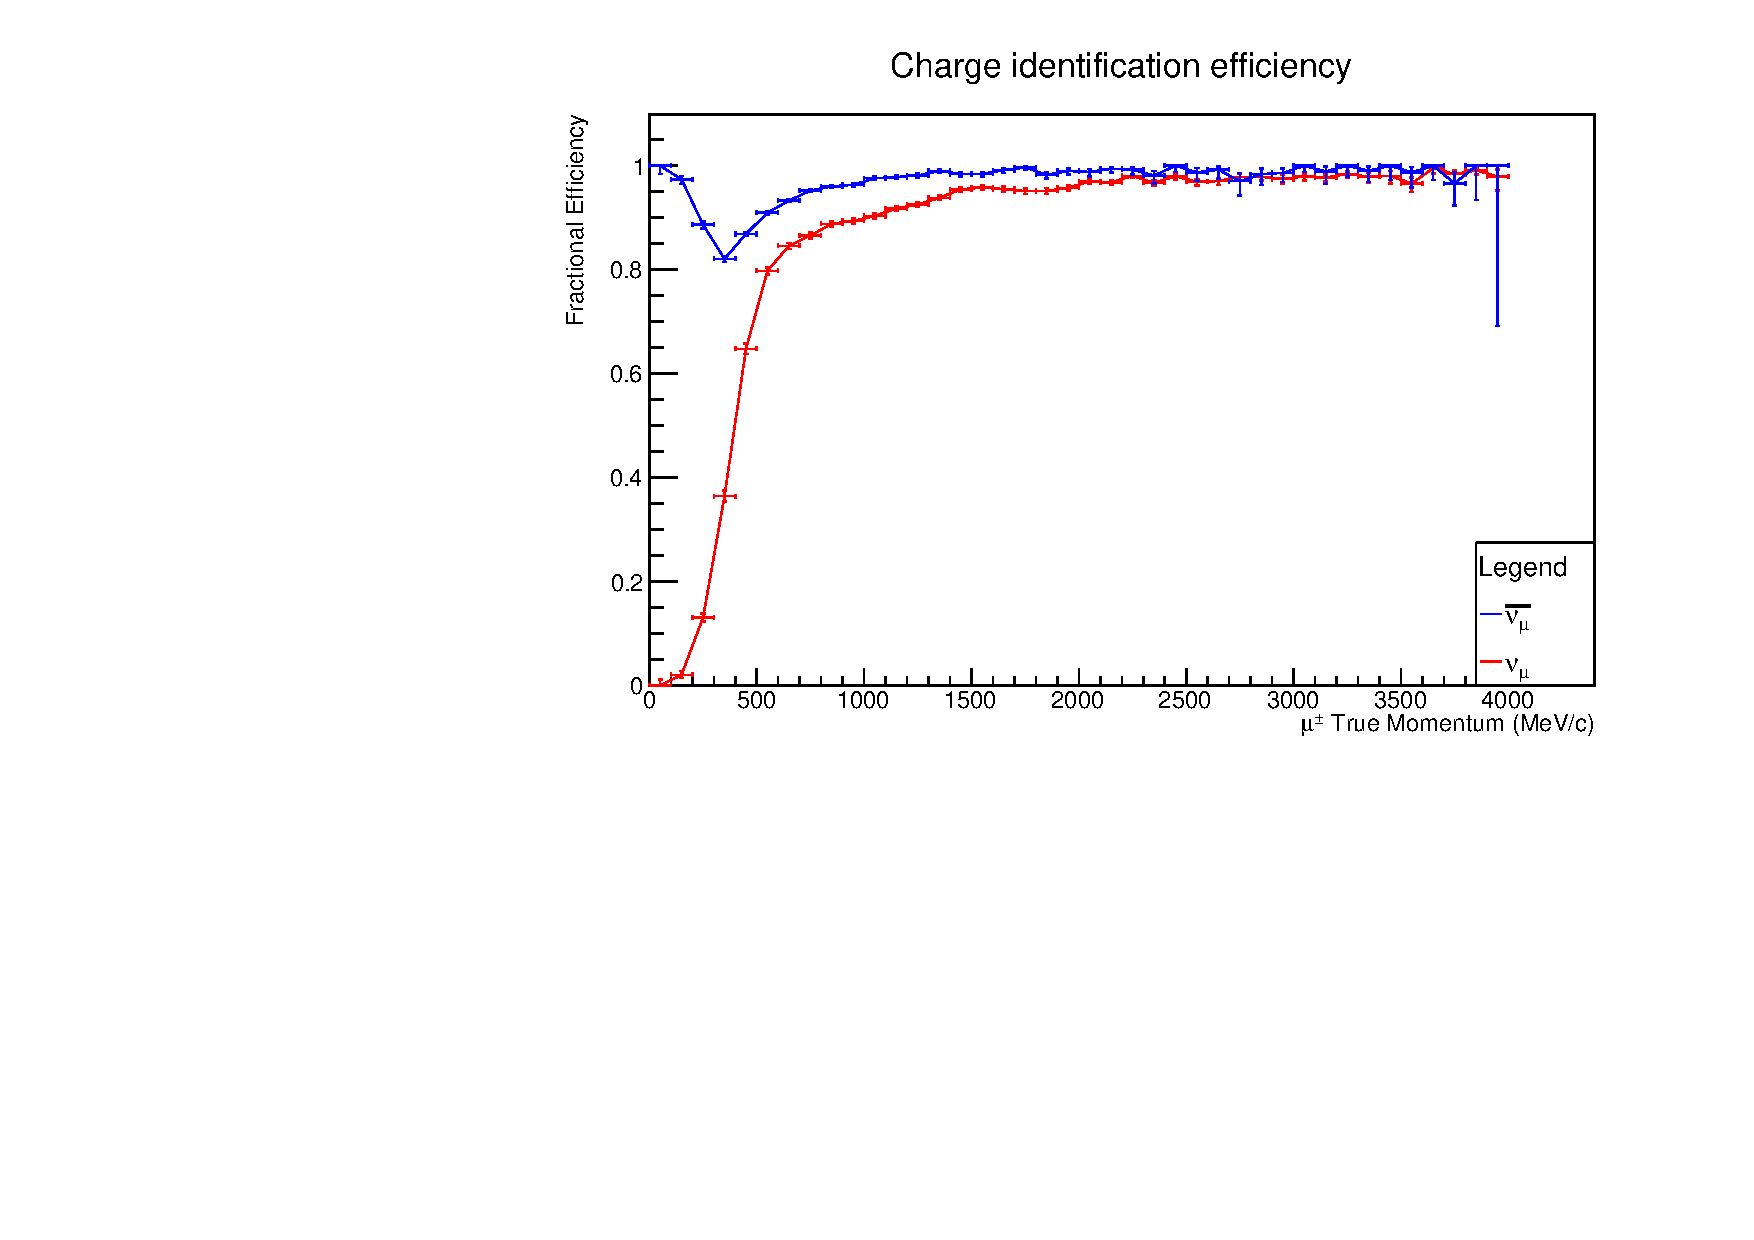
\includegraphics[width=.9\textwidth]{figures/NeutrinoChap/Neutrino/T2KIronChargeEff.pdf}
\caption{Charge reconstruction efficiency showing the efficiency of reconstructing the correct muon charge rom a simulated neutrino charge current event in the first three modules of iron of Baby MIND with respect to the reconstructed track, as a function of muon momenta.}
\label{fig:IronMINDfittedcharge}
\end{figure}

\begin{figure}[h!]
\centering
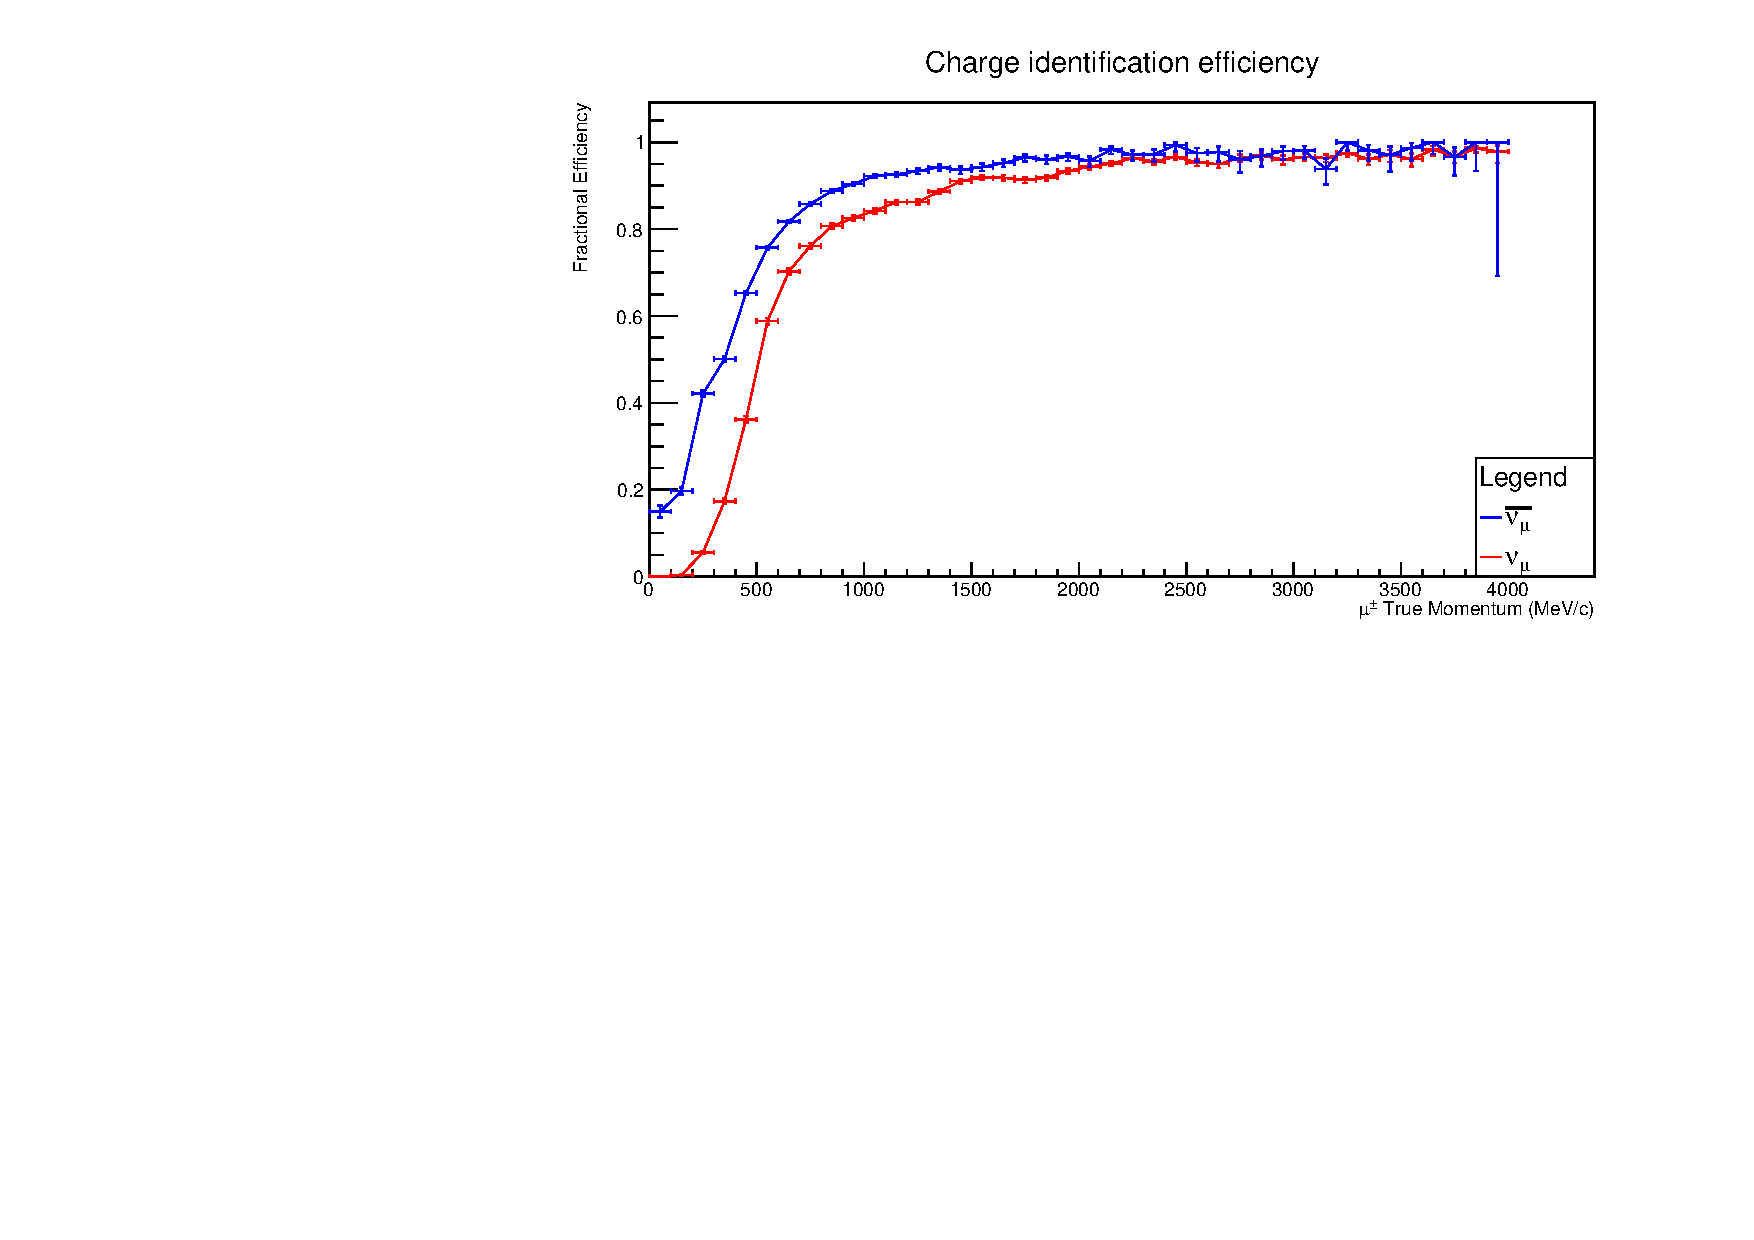
\includegraphics[width=.9\textwidth]{figures/NeutrinoChap/NuFactTalk/fix3.pdf}
%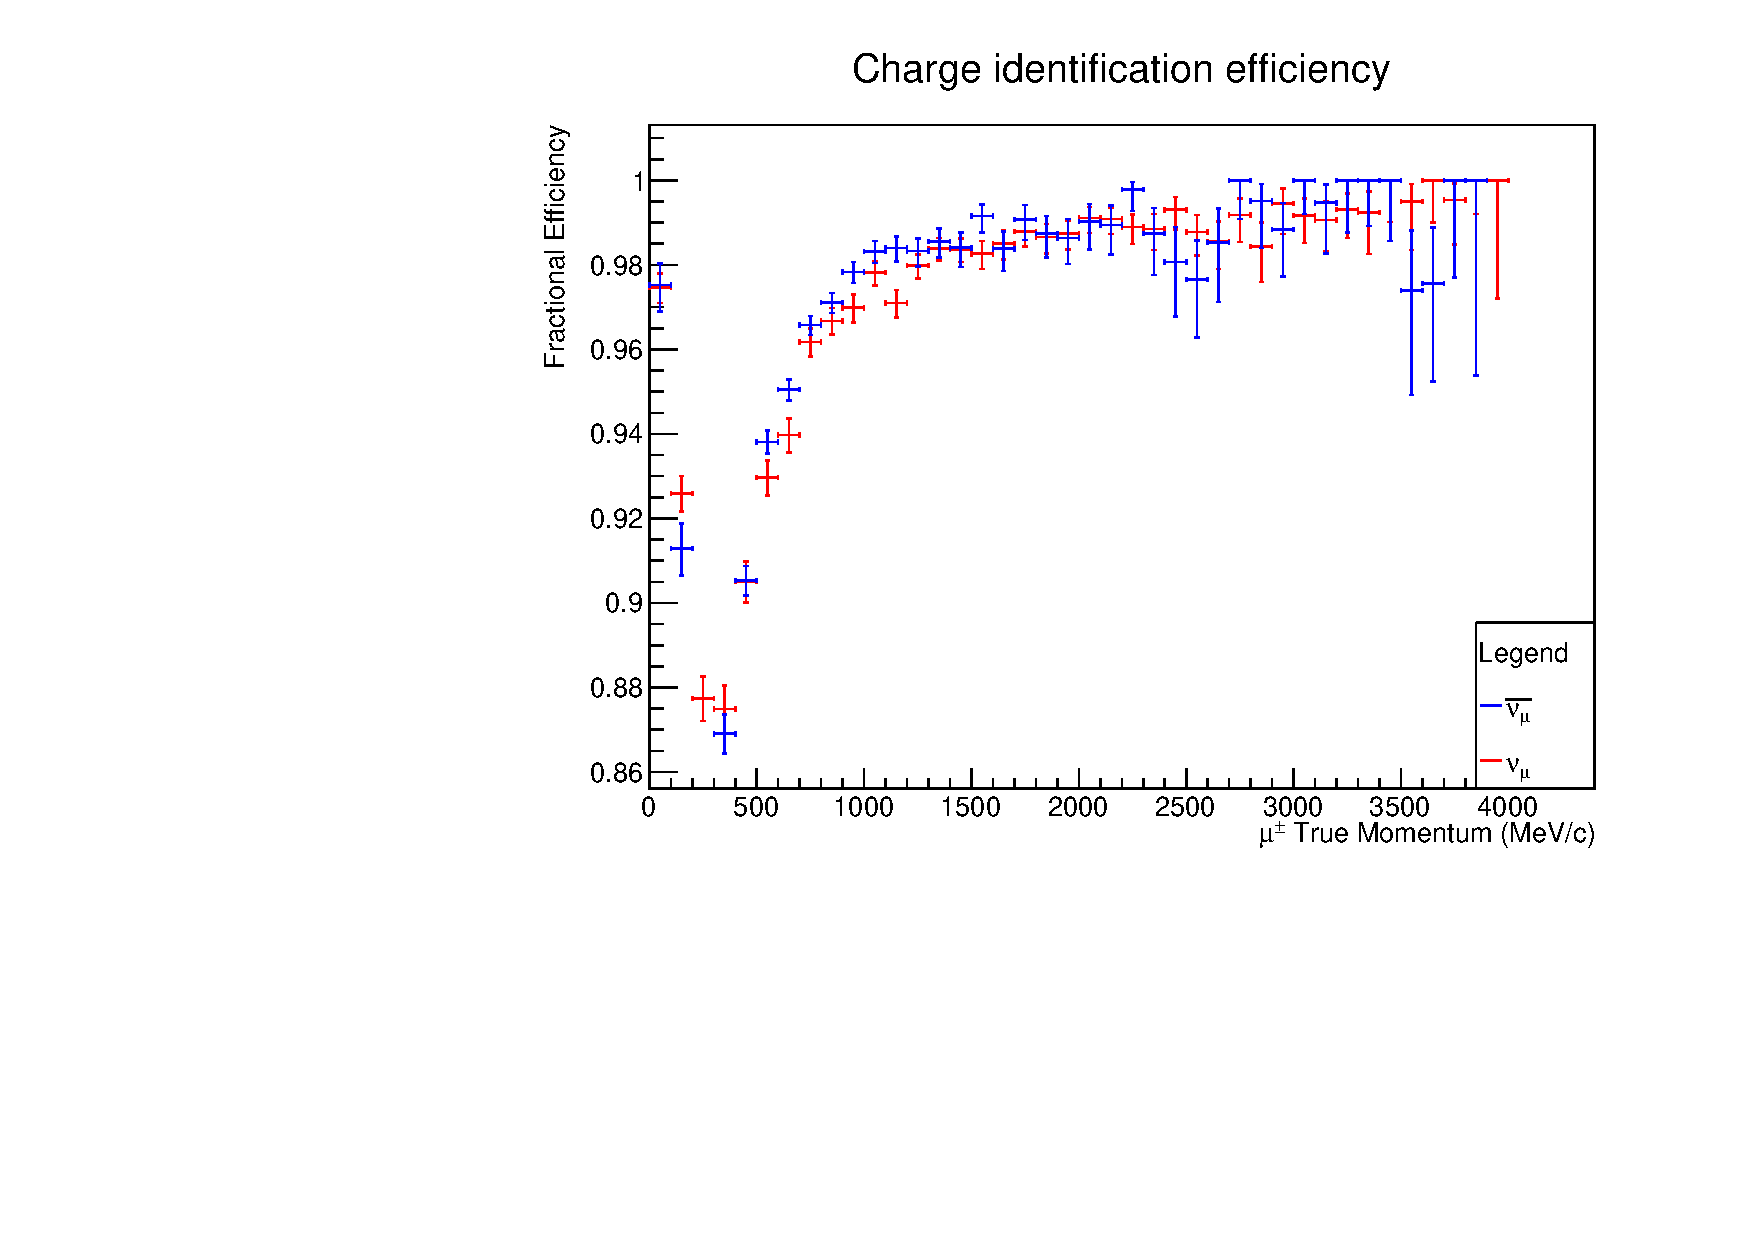
\includegraphics[width=.9\textwidth]{figures/NeutrinoChap/data260618/T2K/ChargeIDT2KNeutrinoBeamMIND.pdf}
\caption{Charge reconstruction efficiency with respect to the originally simulated neutrino interaction in the first three modules of Baby MIND, showing the efficiency of reconstructing the correct muon charge with respect to the simulated neutrino charge current event, as a function of muon momenta. This plot is the multiplication of the efficiencies in figures 7.6 and 7.7. }
\label{fig:IronMINDCombined}
\end{figure}

\begin{figure}[h!]
\centering
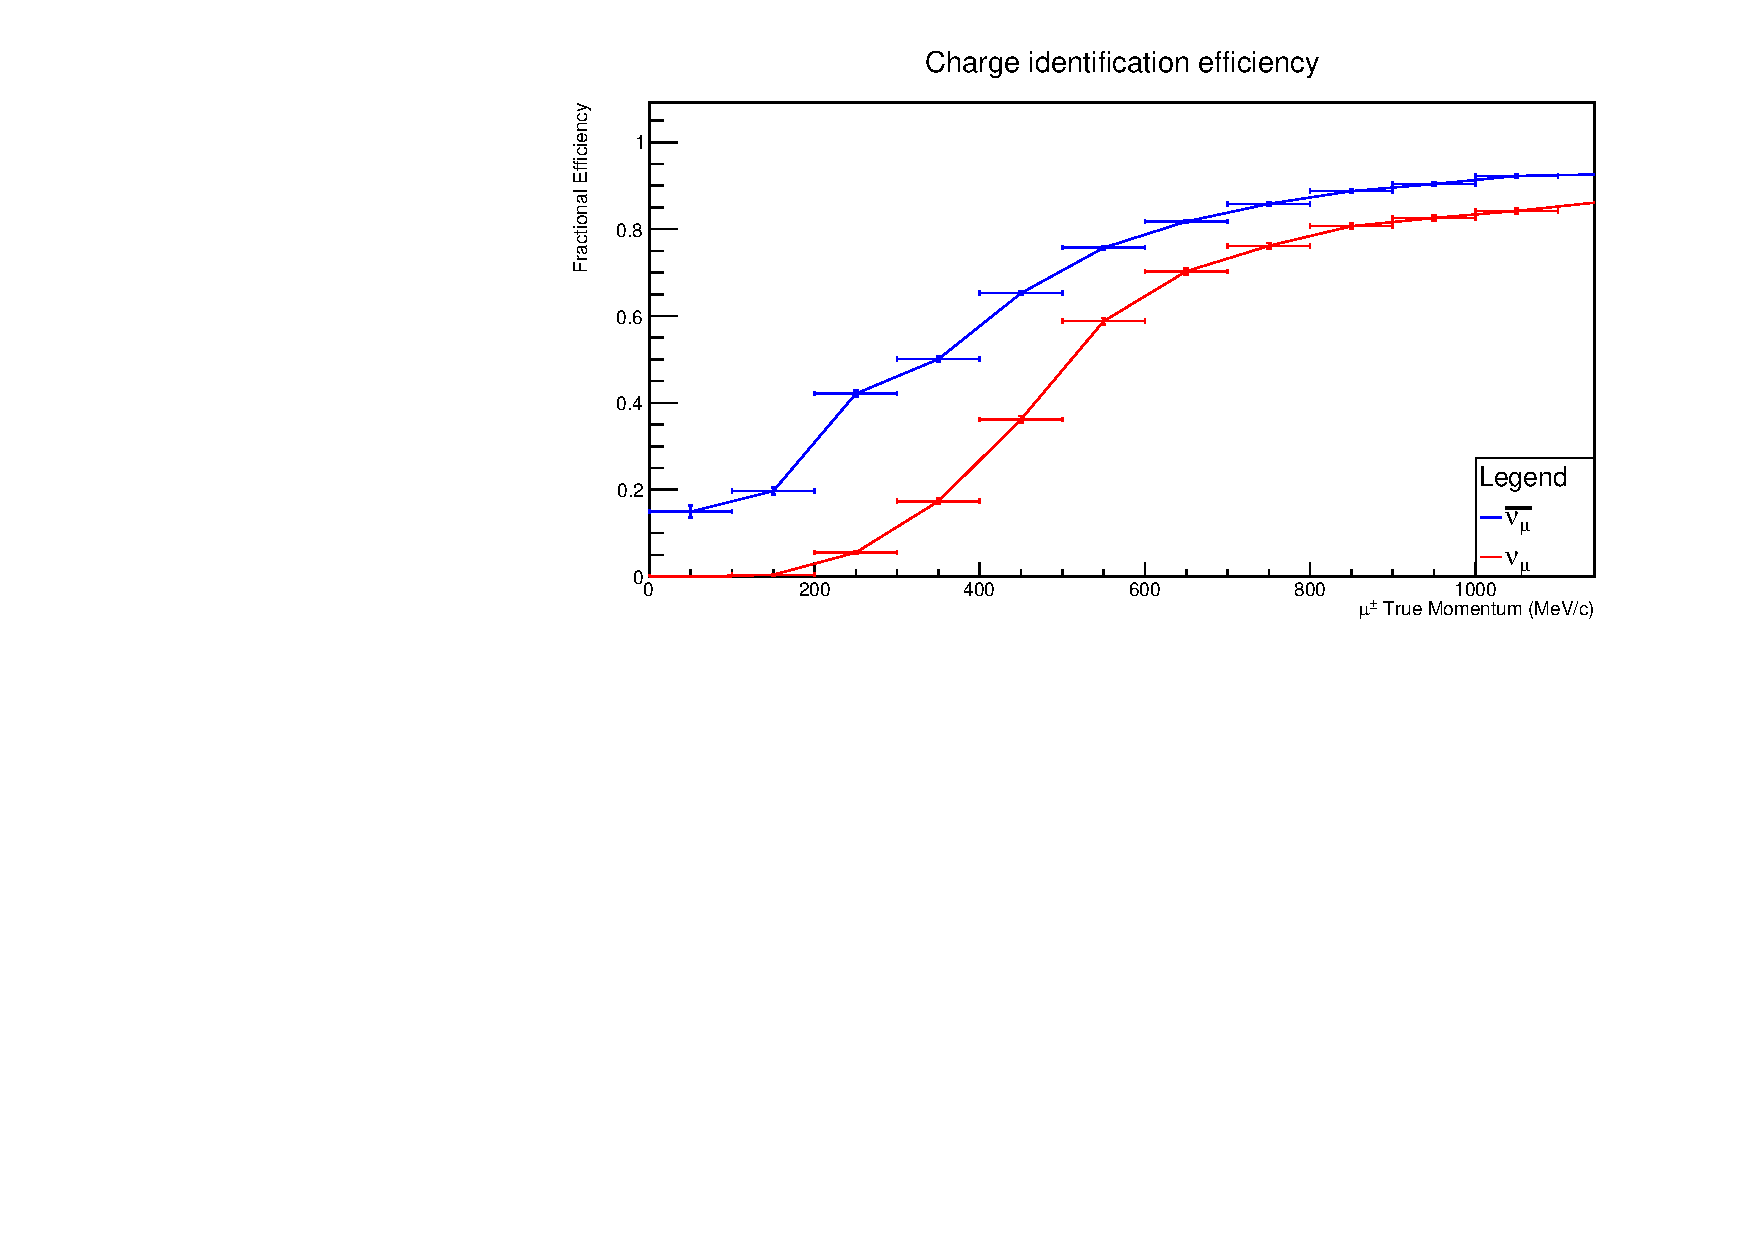
\includegraphics[width=.9\textwidth]{figures/NeutrinoChap/NuFactTalk/fix4.pdf}
%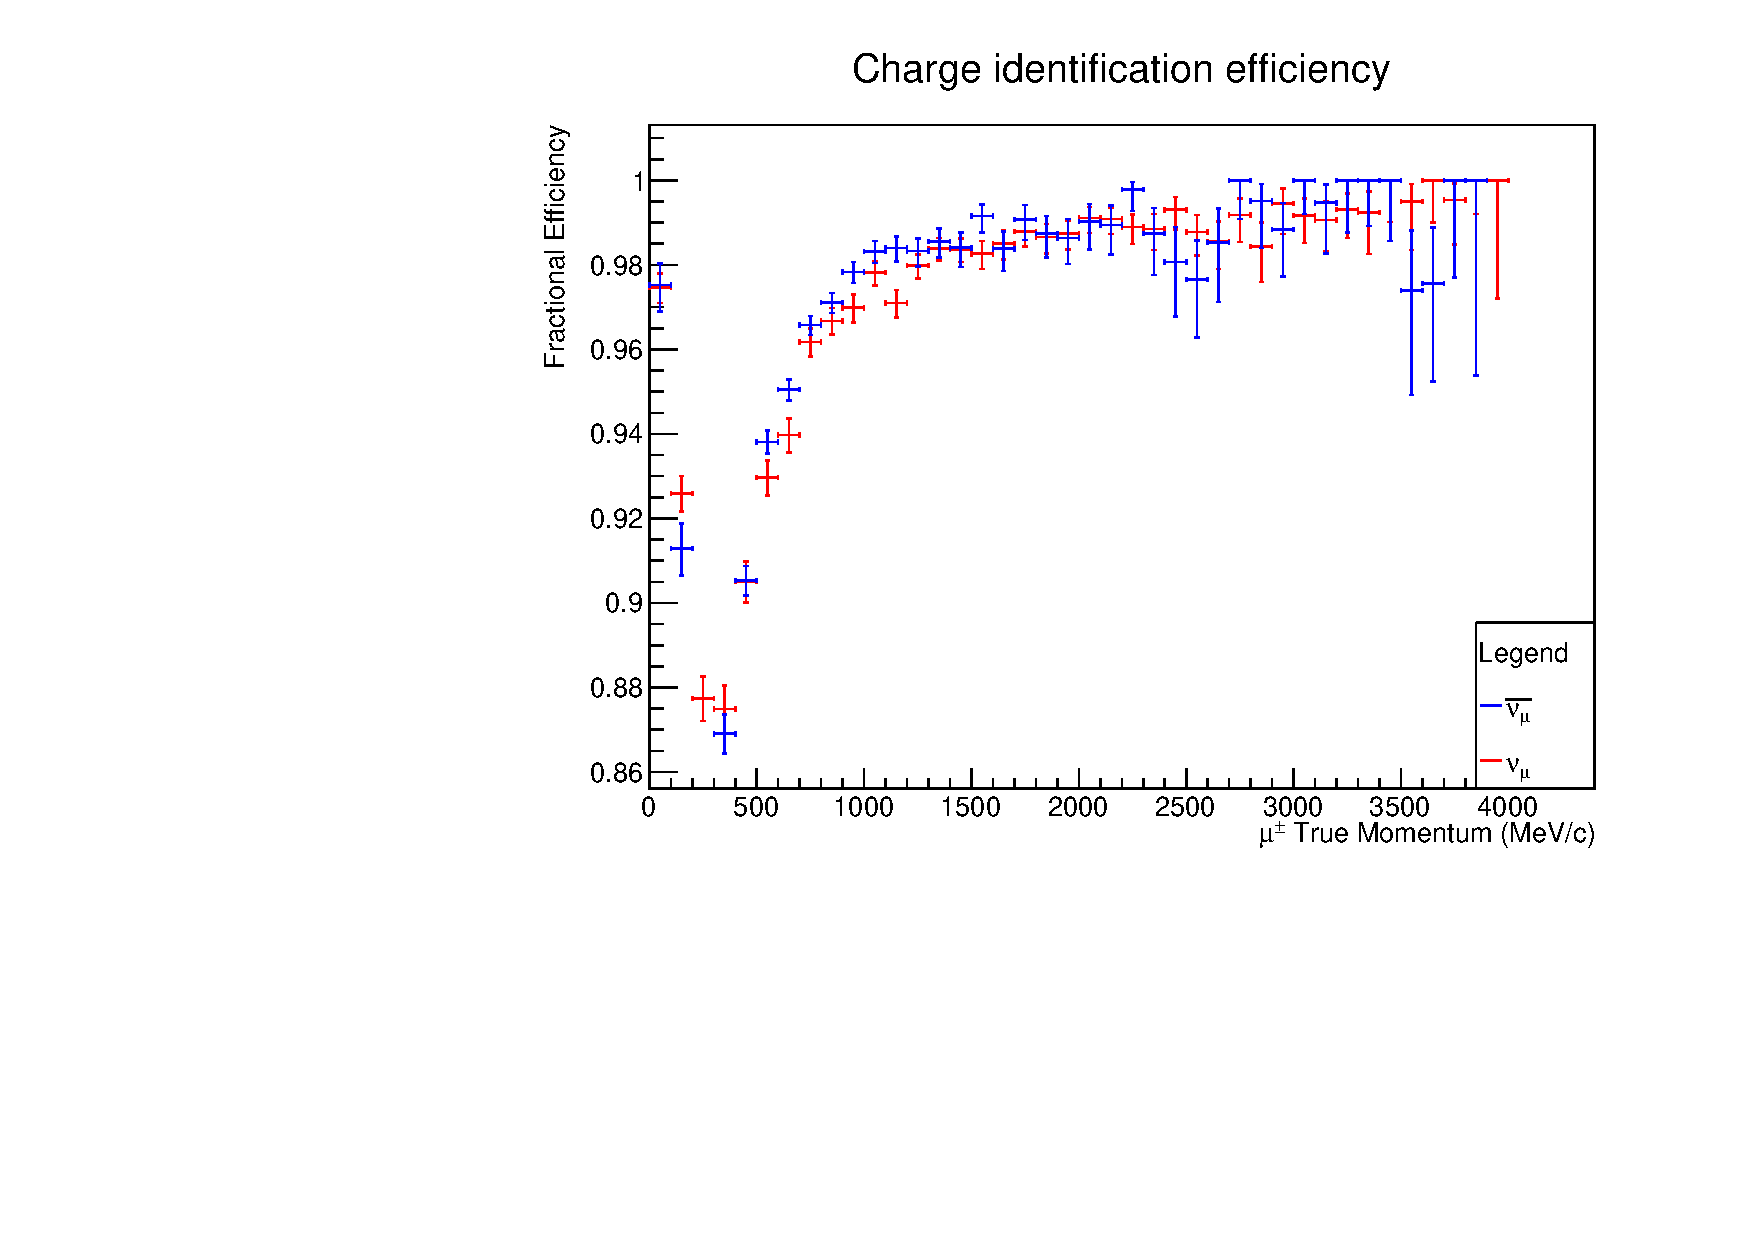
\includegraphics[width=.9\textwidth]{figures/NeutrinoChap/data260618/T2K/ChargeIDT2KNeutrinoBeamMIND.pdf}
\caption{Zoom of figure 7.8, showing the charge reconstruction efficiency with respect to the originally simulated neutrino interactions in the first three  modules of Baby MIND, in the lower momentum range.}
\label{fig:IronMINDCombinedZoom}
\end{figure}



\pagebreak
\newpage
\FloatBarrier
%\subsection{Comparing simulations to data}
\section{Comparison of simulations to data}

%All of this is just one big ramble. Please make this look like a thesis, not some random thoughts. This needs to be tightened up. 

%In this section you need to describe the data that was taken, when it was taken, under what conditions, the dates of the runs, how many days of neutrino data were taken, roughly how many POT were used, what runs were used, the selection criteria, including the trigger condition that was used. 
%After all of this you need to say how many neutrino events survived and how many antineutrino events survived. Then you need to describe how you compare to the simulation. 

%For this you need to show the algorithm that you used, including the equation to estimate the number of antineutrino and neutrino events: Number events = flux * cross section * N_target. 

%Show this calculation, showing which flux you sued, show the plots of the cross section you used and how the multiplication of these gives you estimates for the number of antineutrinos and neutrinos. 

%Then you can show the plot of the number of estimated events overlayed to the data. 

%Try and conclude with a quantitative estimate of the ratio of antineutrino to neutrino events at 1.5 degrees, based on the previous calculations.


Data was collected during March and May 2018. For this study, data collected between the 24th and 31st of May were used. The data was extracted by the unpacking software for the Baby MIND data, found at \url{https://github.com/MrMefodij/BabyMINDunpacking}. The unpacking of the data produced 34675 (100\%) events which were input into the SAURON framework. From this number of events only 9562 (27.6\%) are seen as track-like and were able to be reconstructed. After the events were selected, an angular cut was made requiring the initial track angle with respect to the $z-$axis to be less than 30$^\circ$, thus reducing the number of events to 4585 (13.2\%). The requirement that the momentum was well reconstructed within a range $200~{\rm MeV/c} < p < 10,000~{\rm MeV/c}$, further reduced the number of events to 3899 (11.2\%). After these cuts there are 2245 tracks reconstructed as having a positive charge and 1654 with negative charge. Further imposing the fiducial cuts such as no hits in the first scintillator plane (to remove neutrino interactions upstream of Baby MIND) reduces this number to 2209 (6.4\%) and finally requiring hits in the second, third and fourth scintillator planes provides the final number of events to be 224 (0.6\%). Out of this sample, 123 event are reconstructed with positive charge and 101 with negative charge. Based on the number of reconstructed events and using the statistical error the estimated ratio of antineutrino to neutrino events at 1.5$^\circ$ off axis is $1.22 \pm 0.15$.

To compare data to simulations, two samples of 100000 muon neutrino and antineutrino events each were simulated in the SAURON framework defining the GENIE interaction area to be the same iron plates as described in the fiducial cut. This provided the reconstructed energy spectrum as seen in~\FigRef{fig:SimuSpectrum} with 27926 (27.9\%) neutrino and 33681 (33.7\%) antineutrinos which survive all the cuts.

\begin{figure}[h!]
\centering
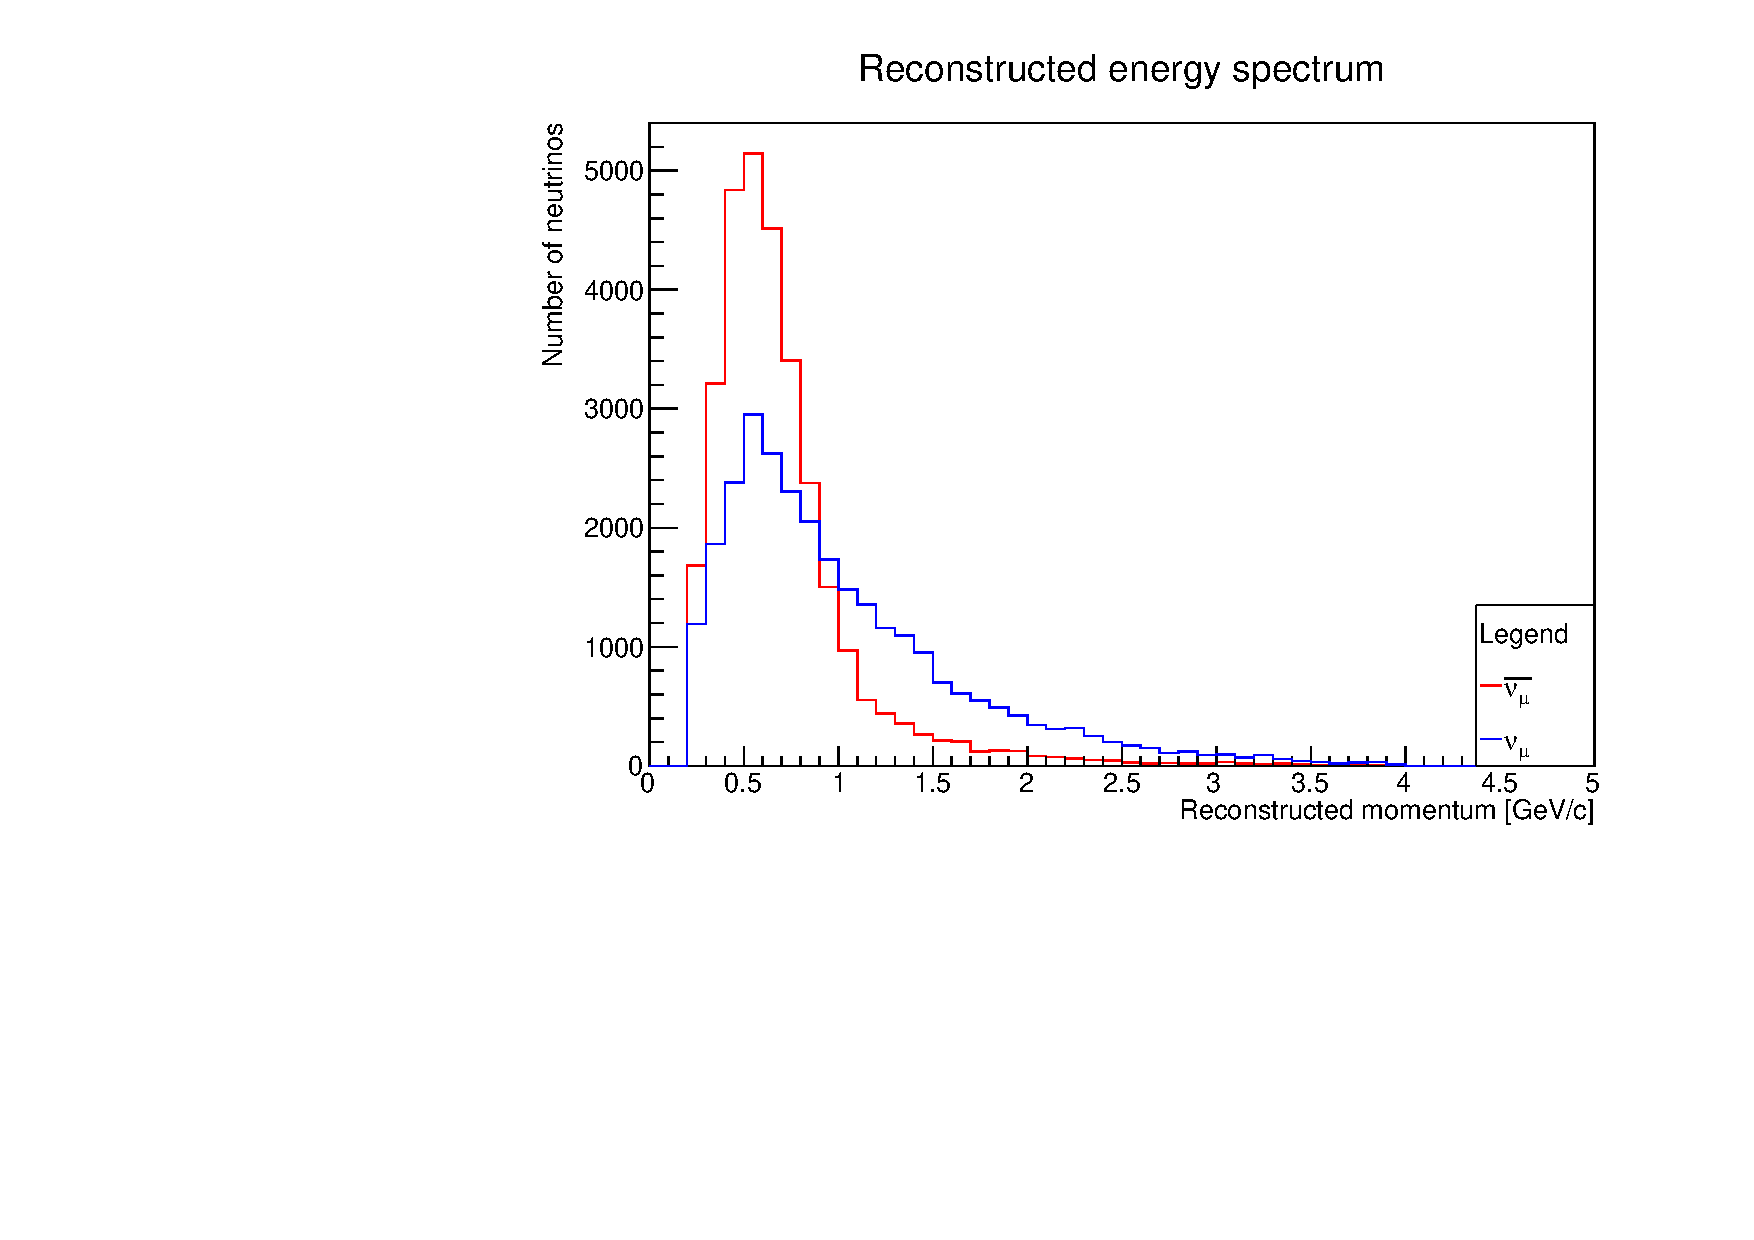
\includegraphics[width=.9\textwidth]{figures/NeutrinoChap/ReconstructedESpectrum.pdf}
%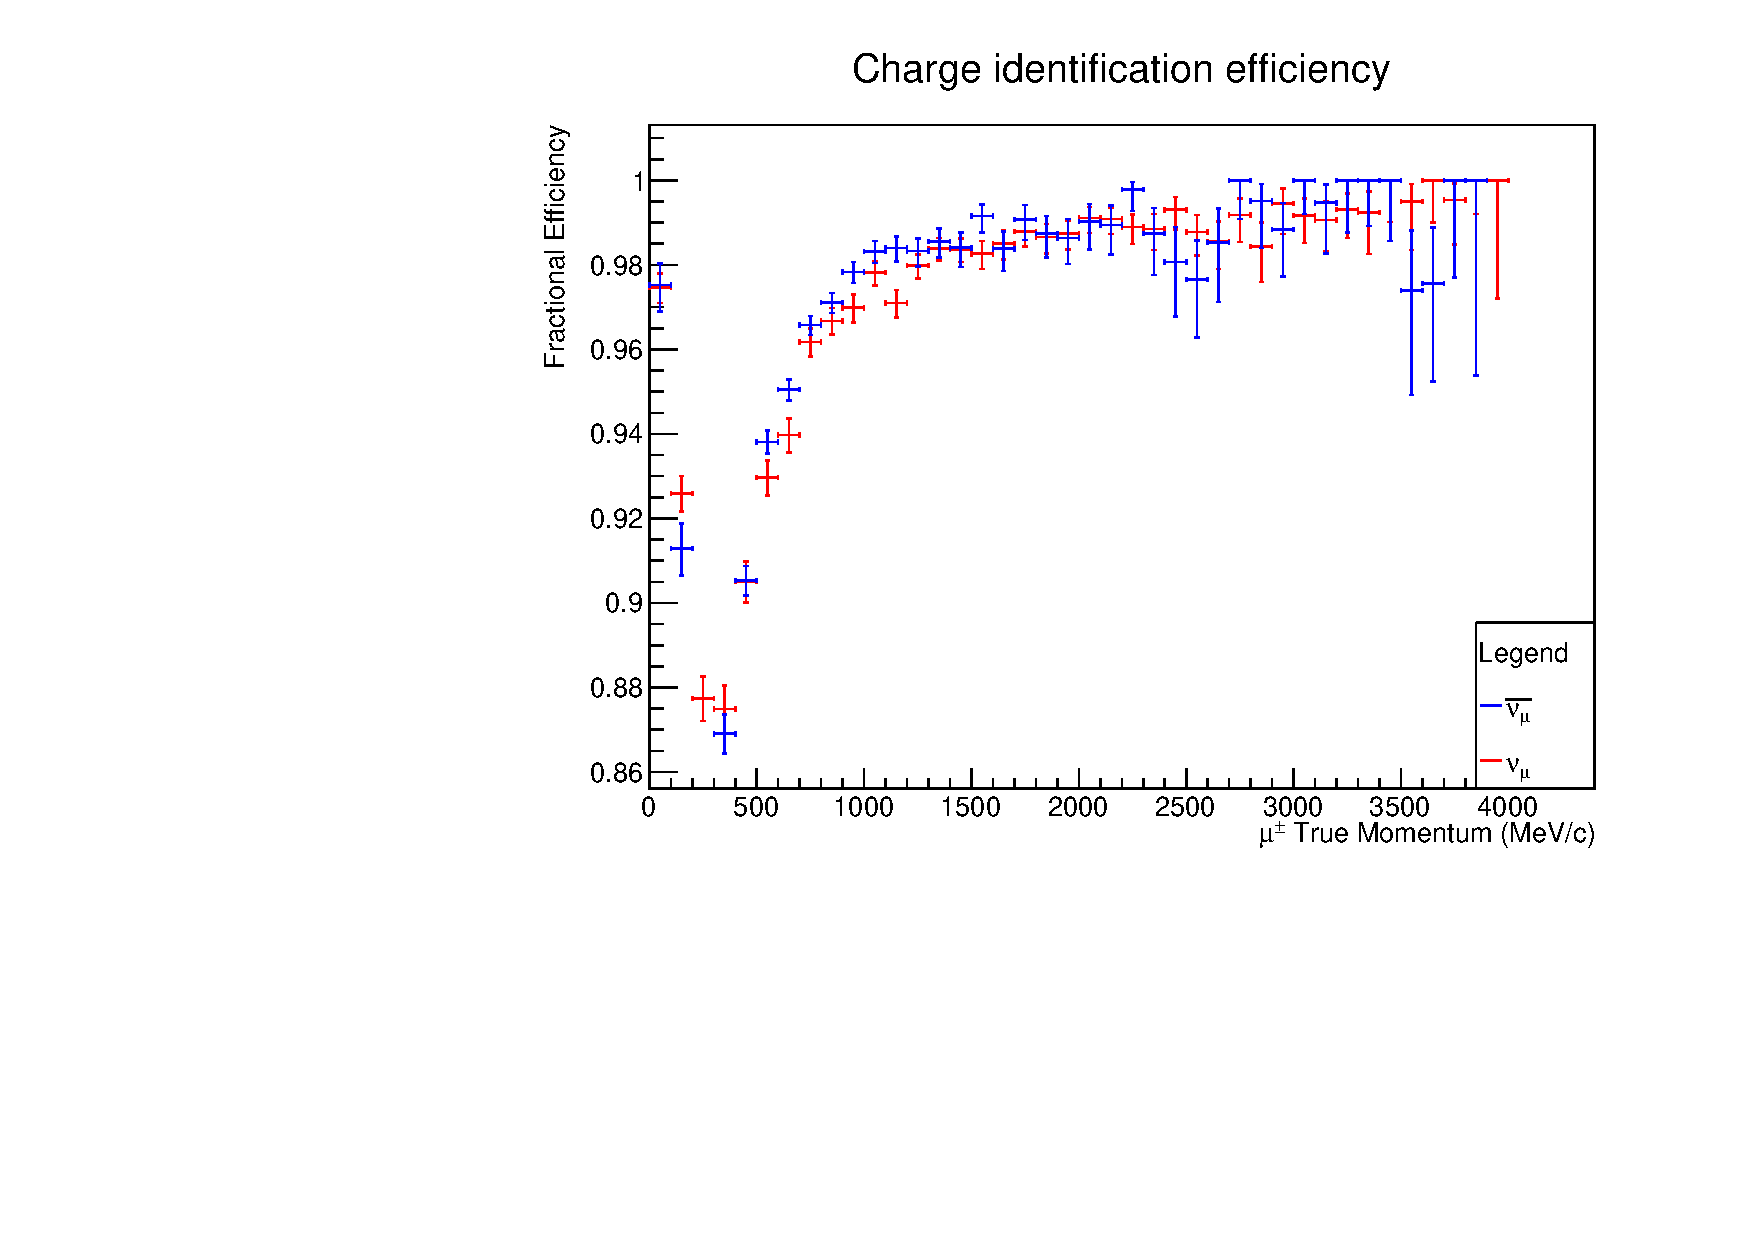
\includegraphics[width=.9\textwidth]{figures/NeutrinoChap/data260618/T2K/ChargeIDT2KNeutrinoBeamMIND.pdf}
\caption{The reconstructed energy spectrum for the simulated neutrino events in SAURON.}
\label{fig:SimuSpectrum}
\end{figure}

The simulated reconstructed energy spectrum needs to be converted to number of events. This is done through the following equation:
\begin{equation}
N_{events} = \int \phi_\nu(E) \times \sigma(E) \times N_{target} dE
\end{equation}
%N_{events} = \phi_\nu \times \sigma \times N_{target}
where $\phi(E)$  is the neutrino flux as a function of neutrino energy $E$, seen in ~\FigRef{fig:SimuFlux}, $\sigma(E)$ is the neutrino and antineutrino total cross sections taken from figures~\ref{fig:neutrinoInteractionsFig} and~\ref{fig:antineutrinoInteractionsFig} and $N_{target}$ is the number of iron nucleons in a 1500 kg mass which is $N_{target}=9.03 \times 10^{29}$. This provides the total number of neutrino events as 7588 muon neutrinos and 23432 muon antineutrinos for 1500 kg of iron and $10^{21}$ POT. Combining these results with the reconstruction efficiency provides 2117 muon neutrinos and 7899 muon antineutrinos reconstructed with the correct charge for 1500 kg of iron and $10^{21}$ POT. The expected ratio of neutinos to antineutrinos is $3.7$, which is different to the observed ratio of $1.22$ in the data. This discrepancy is under investigation. 

%However, when the neutrino simulations are normalized to the neutrino data and the antineutrino simulations are normalized to the antineutrino data, the momentum distribution agrees well as can be seen in~\FigRef{fig:datanumubar} and \FigRef{fig:datanumu}.

 %as seen in~\FigRef{fig:NumSim}.

%This provides a rescaling of the energy spectrum and provides the total number of events in~\FigRef{fig:NumSim}.

\begin{figure}[h!]
\centering
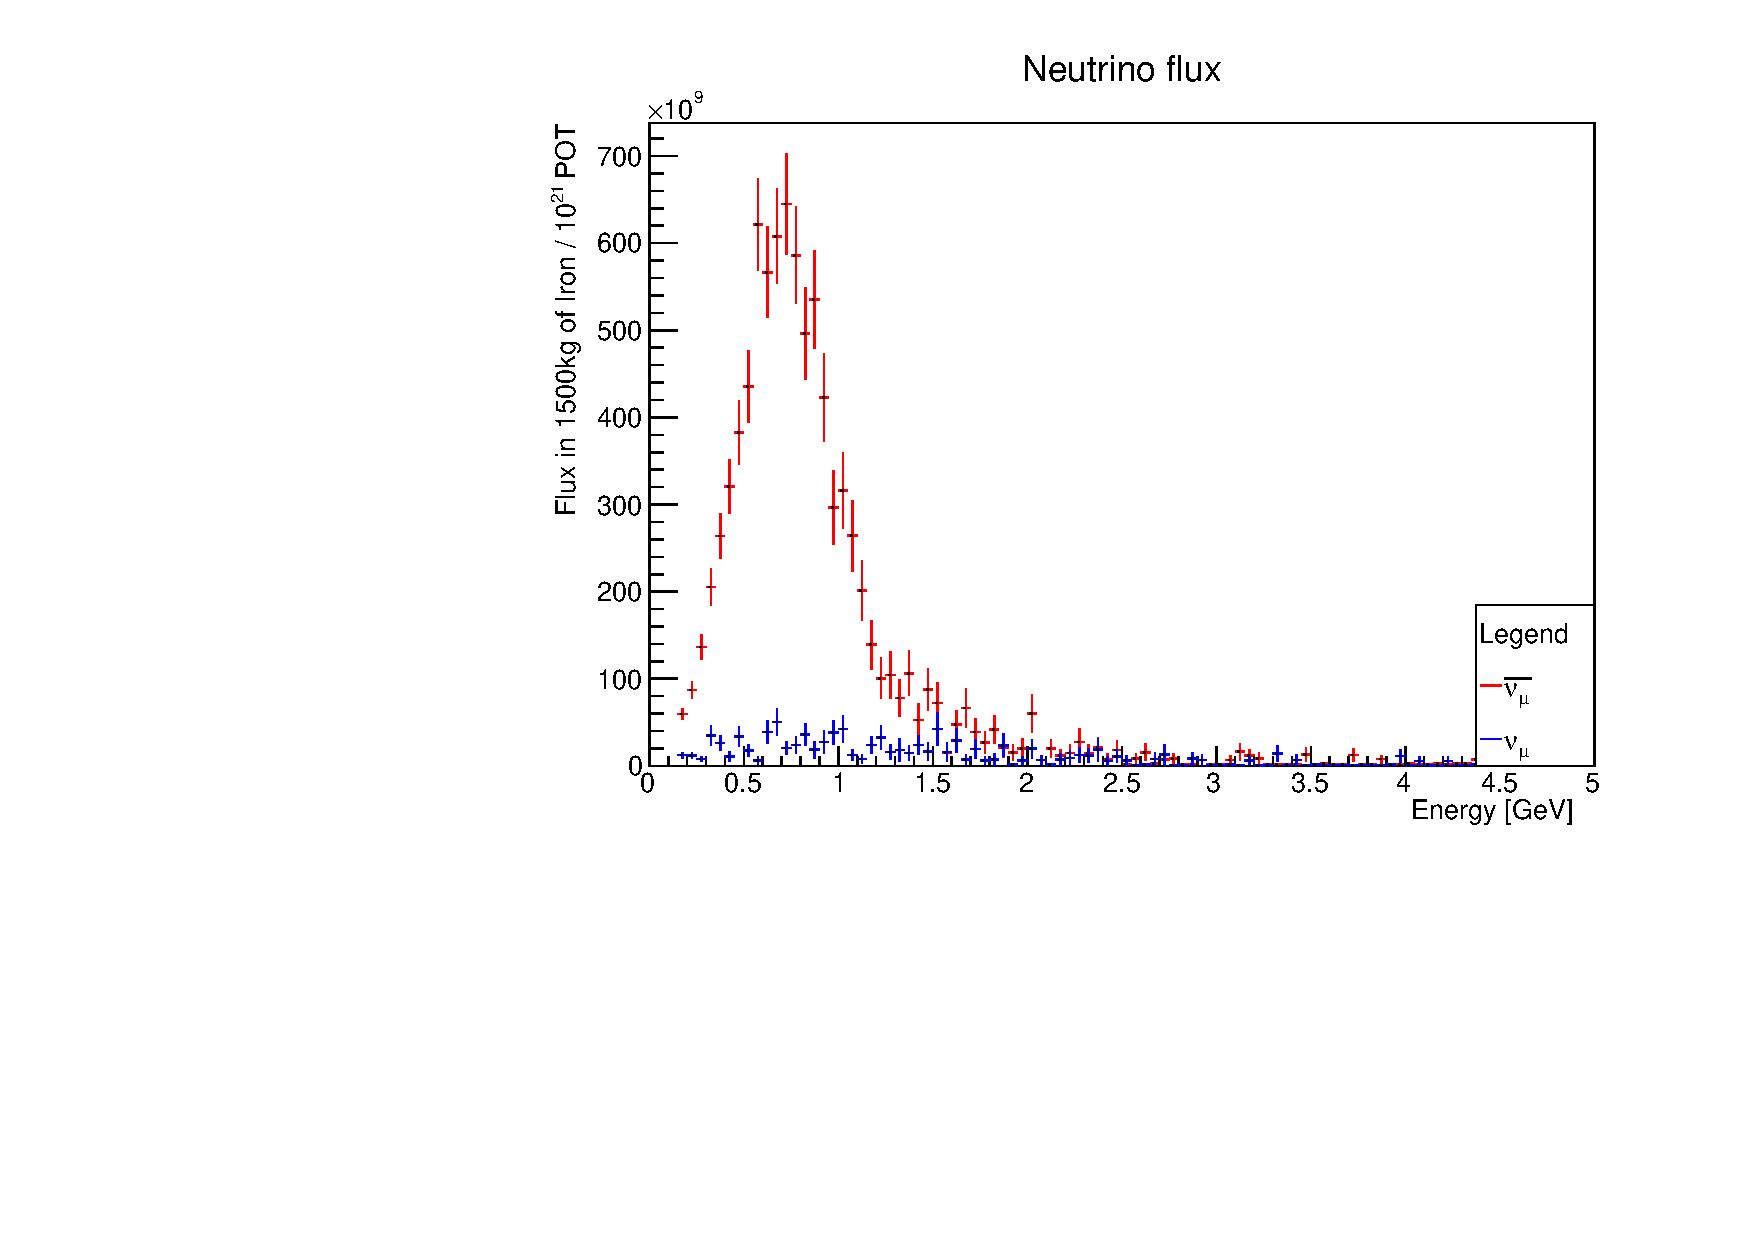
\includegraphics[width=.9\textwidth]{figures/NeutrinoChap/FluxSpectrum.pdf}
%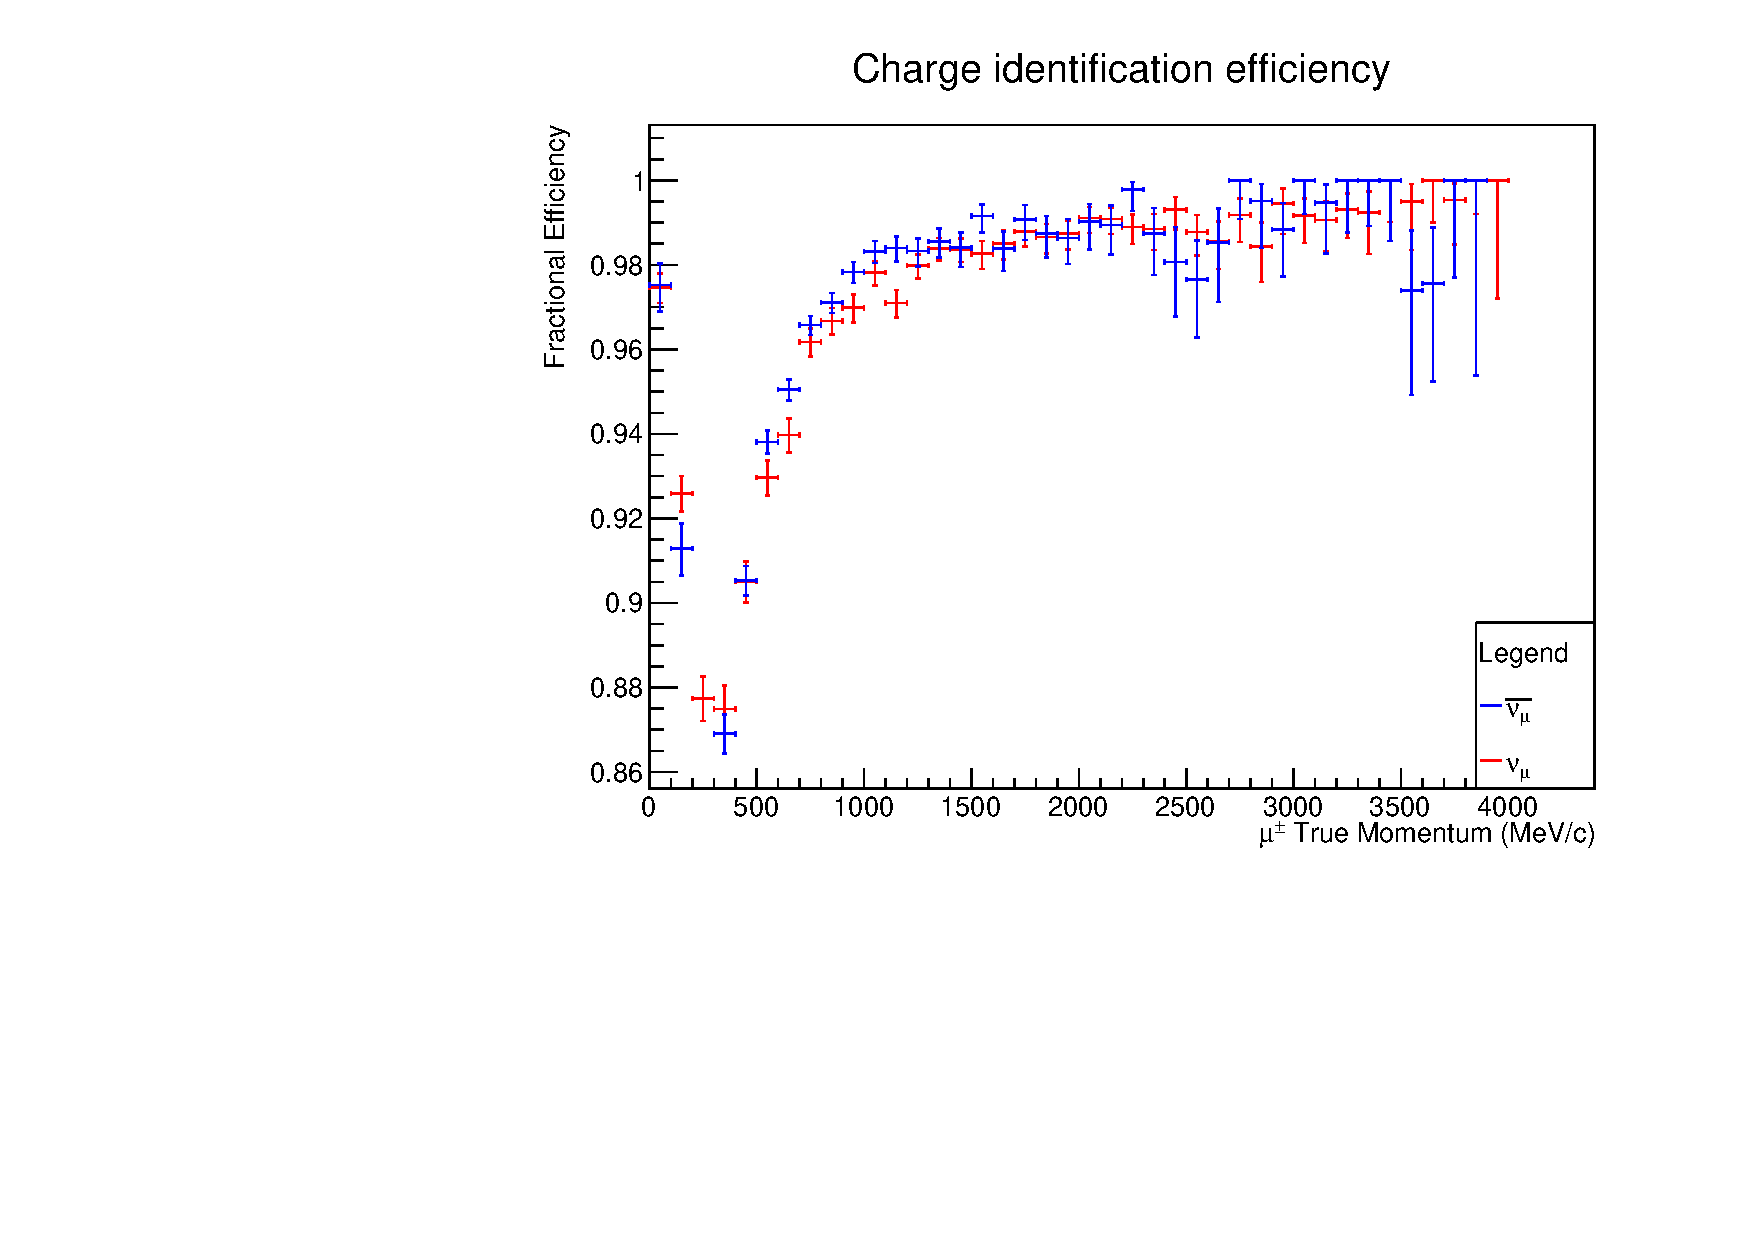
\includegraphics[width=.9\textwidth]{figures/NeutrinoChap/data260618/T2K/ChargeIDT2KNeutrinoBeamMIND.pdf}
\caption{The neutrino flux for $\bar{\nu}_\mu$ and $\nu_\mu$. Figure, courtesy of Kenji Yasutome.}
\label{fig:SimuFlux}
\end{figure}

\if{0}
\begin{figure}[h!]
\centering
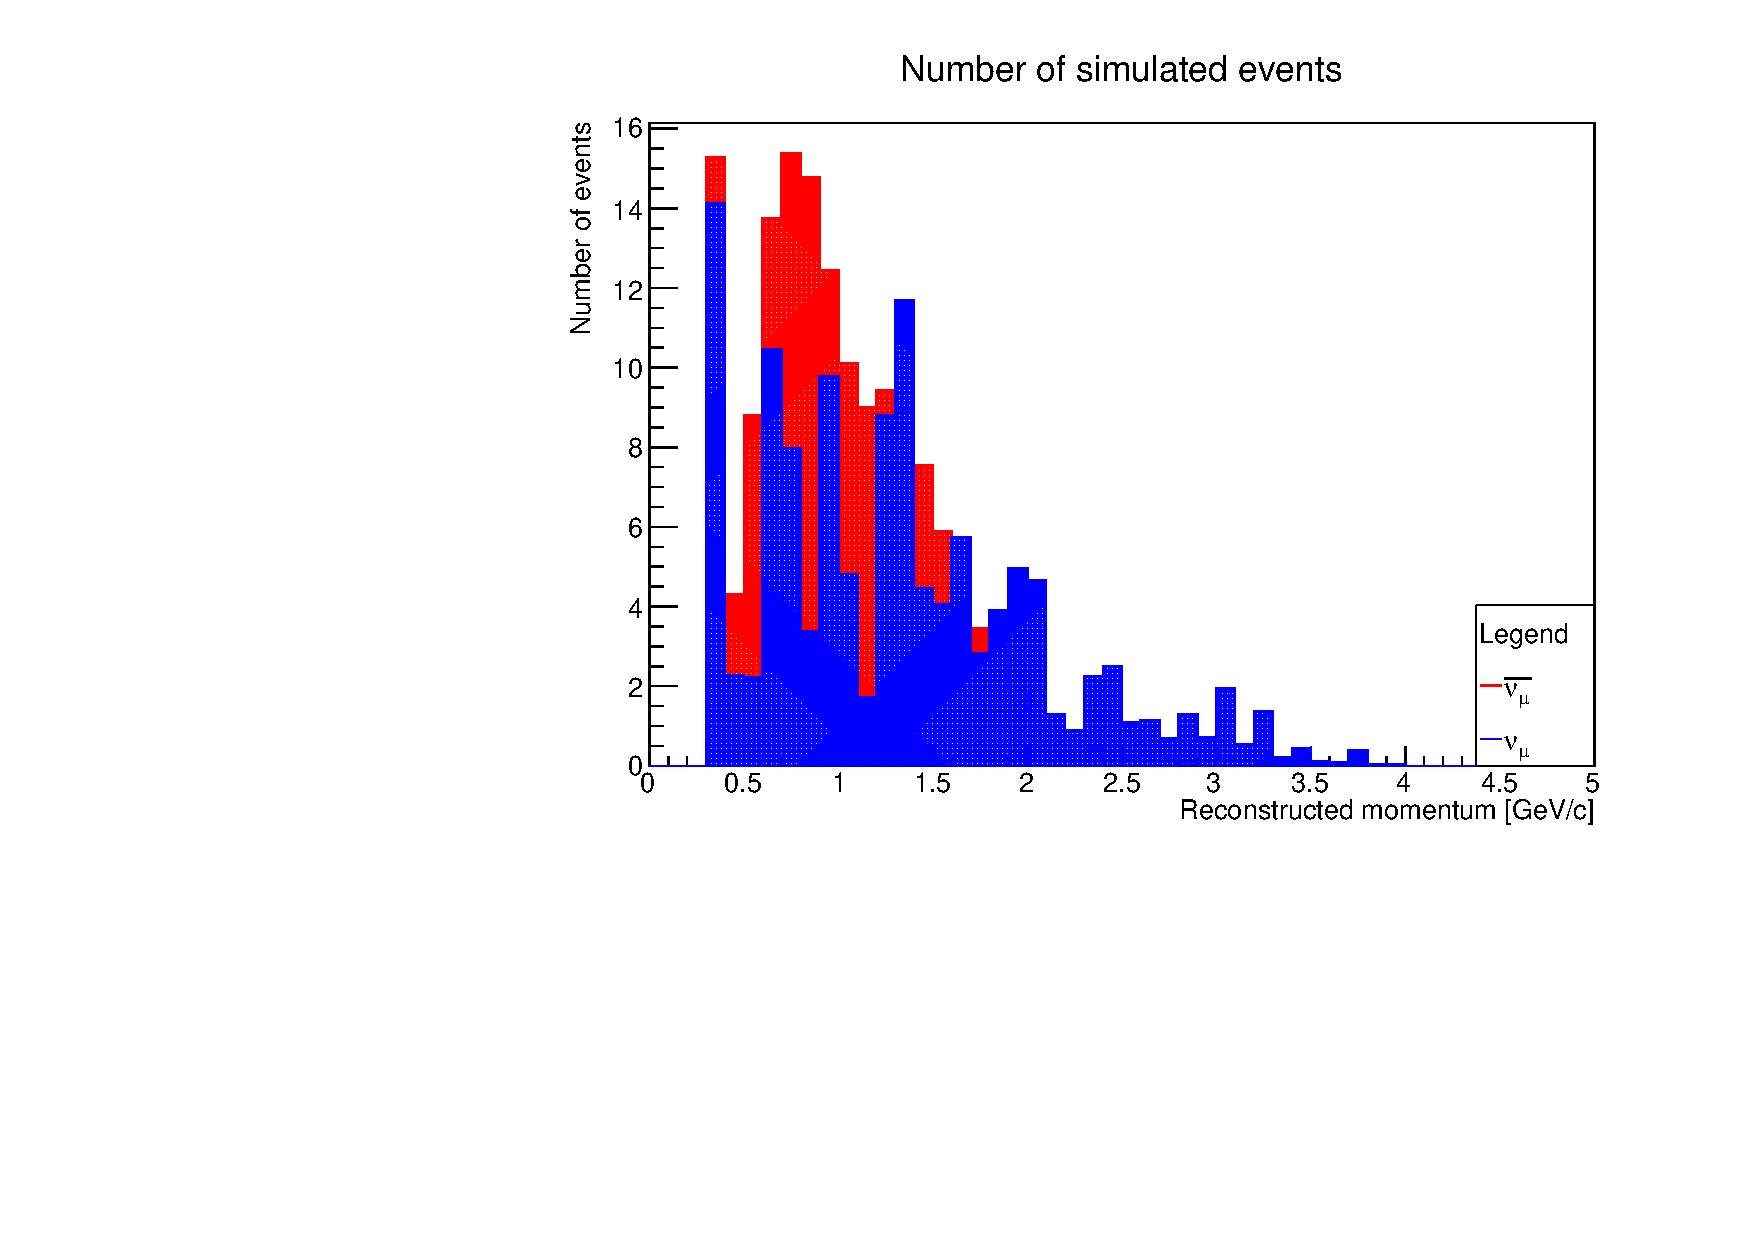
\includegraphics[width=.9\textwidth]{figures/NeutrinoChap/NumSimEvents.pdf}
%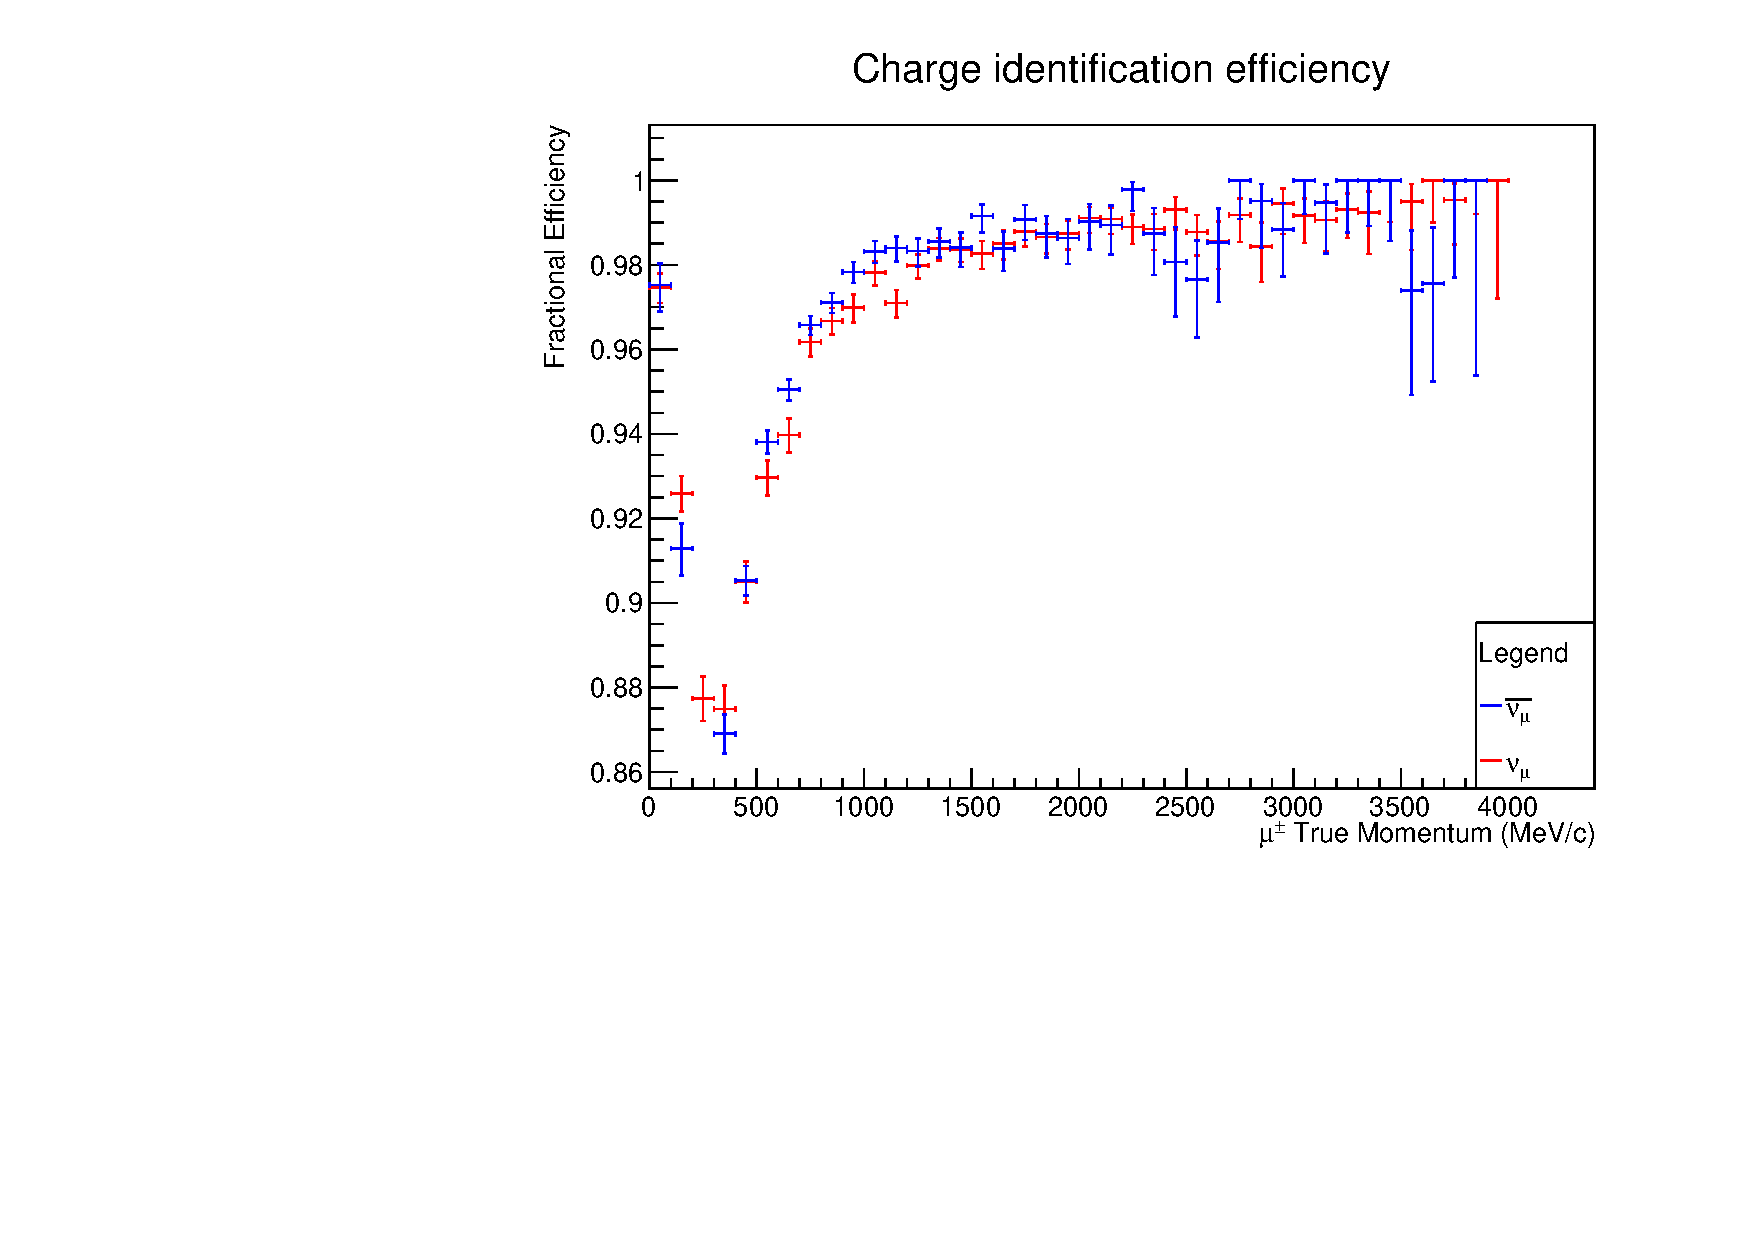
\includegraphics[width=.9\textwidth]{figures/NeutrinoChap/data260618/T2K/ChargeIDT2KNeutrinoBeamMIND.pdf}
\caption{The reconstructed number of simulated neutrino events in SAURON.}
\label{fig:NumSim}
\end{figure}
\fi

%In comparing data to simulations the main way is looking at the reconstructed energy spectra for the events which have been classified as muon neutrino and muon antineutrino respectively. 

The reconstructed energy spectra for events which have been classified as muon neutrinos and muon antineutrinos were compared to the simulations. In \FigRef{fig:datanumubar} and \FigRef{fig:datanumu} the simulated (expected) reconstructed energy spectrum is plotted with the recorded data points extracted from the neutrino beam overlayed. Both plots have been normalized to each other to ensure that the number of simulated events have been scaled to match the number of recorded events.
%The large first bin for the simulation is attributed to the lower momentum events being combined in the lowest bin. 
The results shown in~\FigRef{fig:datanumubar} show good agreement between data and simulations for muon antineutrino events. The results shown in~\FigRef{fig:datanumu} show good agreement between data and simulations for muon neutrino events. %The rough shape is due to the initial flux of neutrinos in RHC being low compared to the antineutrino flux. 

%The large first bin for the simulation is attributed to the lower momentum events being combined in the lowest bin and the further shape is rough due to the initial flux of neutrinos in RHC being low compared to the antineutrino flux. 
%This discrepancy is probably due to differences in reconstruction efficiency in real events, due to inefficiencies in the data collection due to the electronics or the assumption that the muon events have been correctly identified as charge-current events in the iron. It is possible that the cuts need to be enhanced to provide improved results. 

%More neutrino beam data will be collected in 2019 with the Baby MIND detector integrated into the WAGASCI detector.


%For further results more data needs to be collected and data in the forward horn current mode.

%Only data taken during the commissioning phase, some errors in data taking requiring only able to use some data. Not possible to correlate time of events with neutrino events allowing background neutrino events and muons to enter into the data sample.

%Currently only have data for RHC, $\bar{\nu_{\mu}}$. Need to understand deviation and perhaps enforce stricter cuts on data. The main issues seem to be in the uncertainty in the data where an issue comes from not seeing interaction in the iron. The only way to improve on this would be to correlate the beam bunch timing with the data taking. 

%In general, for neutrino interactions a combined analysis will allow for better neutrino event classification. In this analysis all tracks were assumed to be muons from CCQE which does not have to be the case, however the vertex needs to be inspected or more data collected to be able to perform an interaction identification using TMVA. 

%To see vertex WAGASCI is needed.


%Show same as the idea for nuFact, explain in detail what was done. Show the data, neutrino energy reconstruction.


\begin{figure}[h!]
\centering
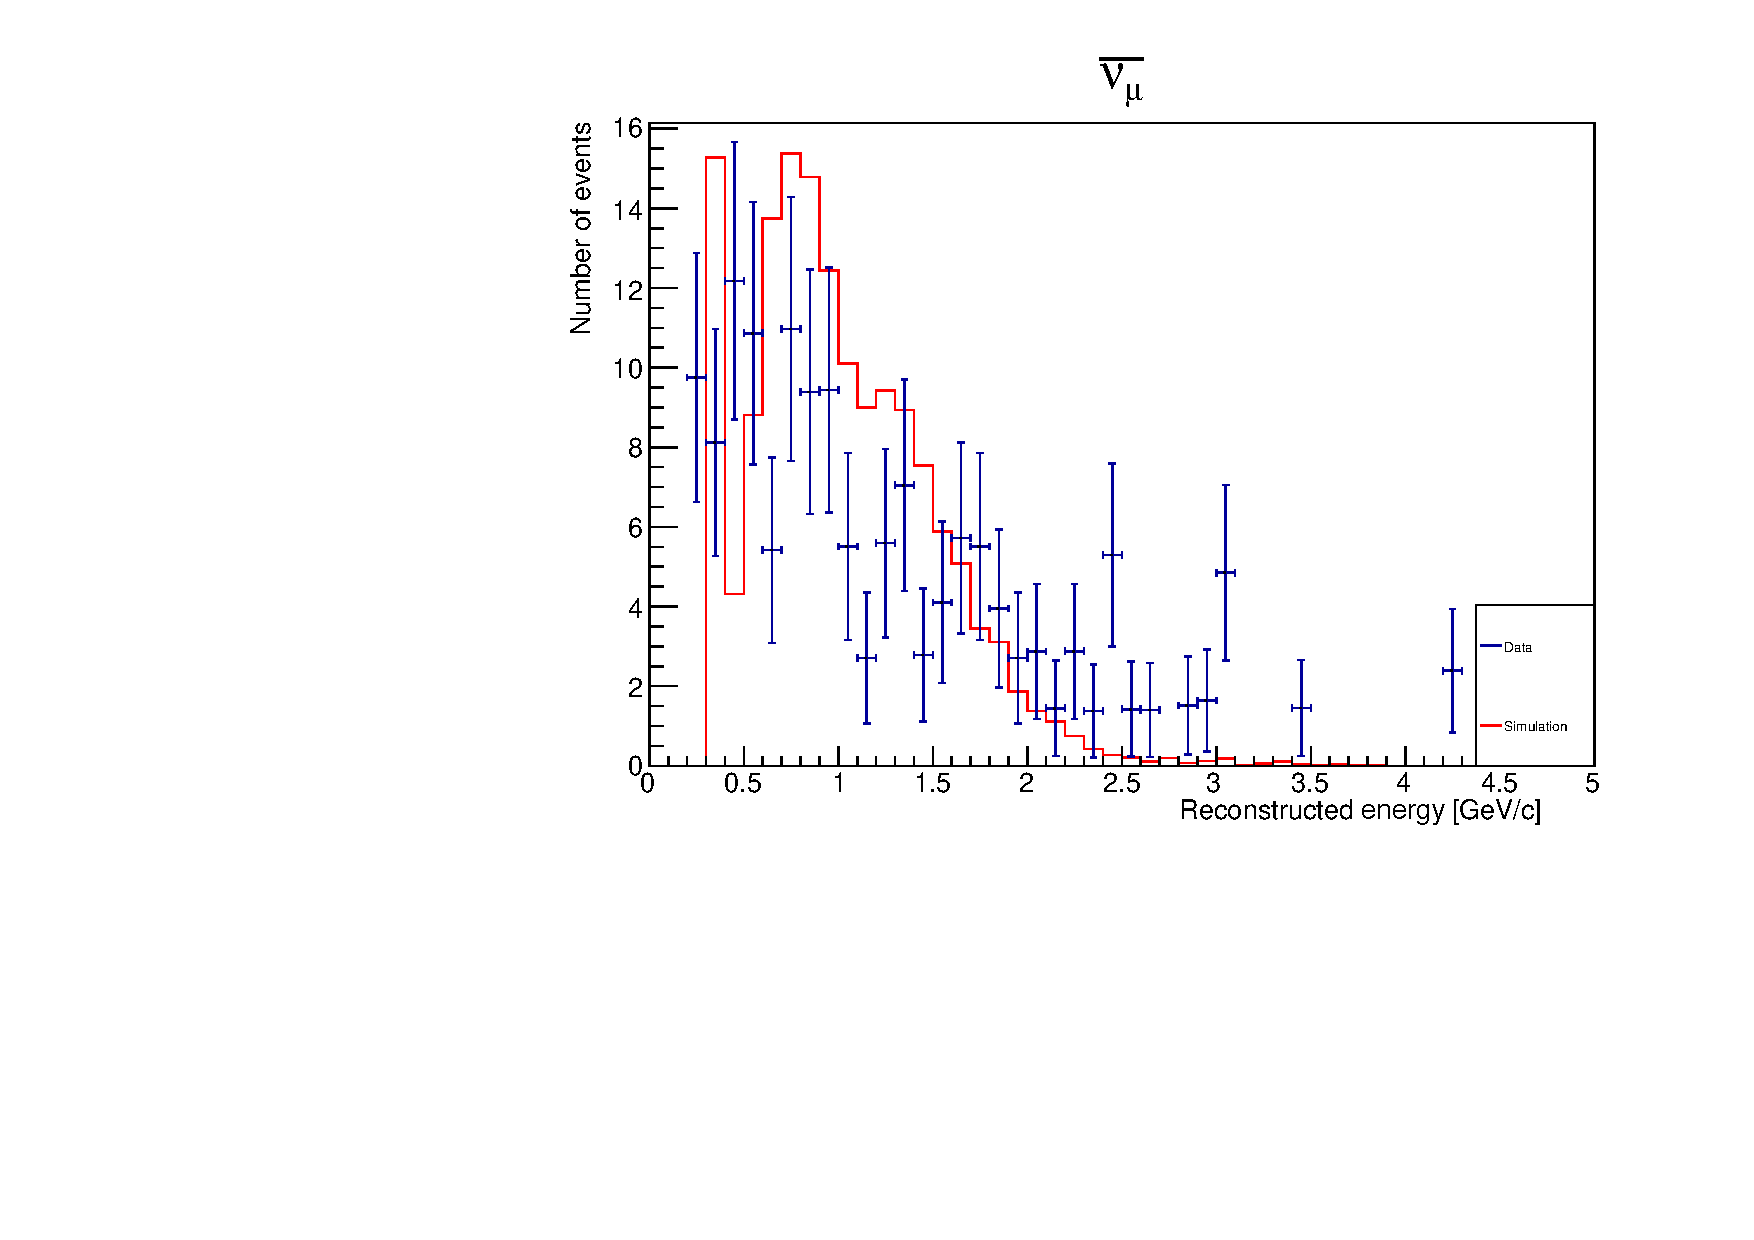
\includegraphics[width=.9\textwidth]{figures/NeutrinoChap/nuBarEventNewest.pdf}
\caption{Energy spectrum of the reconstructed antineutrino $\bar{\nu}_\mu$ events in data (points with error bars) compared to the simulation (histogram).}
\label{fig:datanumubar}
\end{figure}

\begin{figure}[h!]
\centering
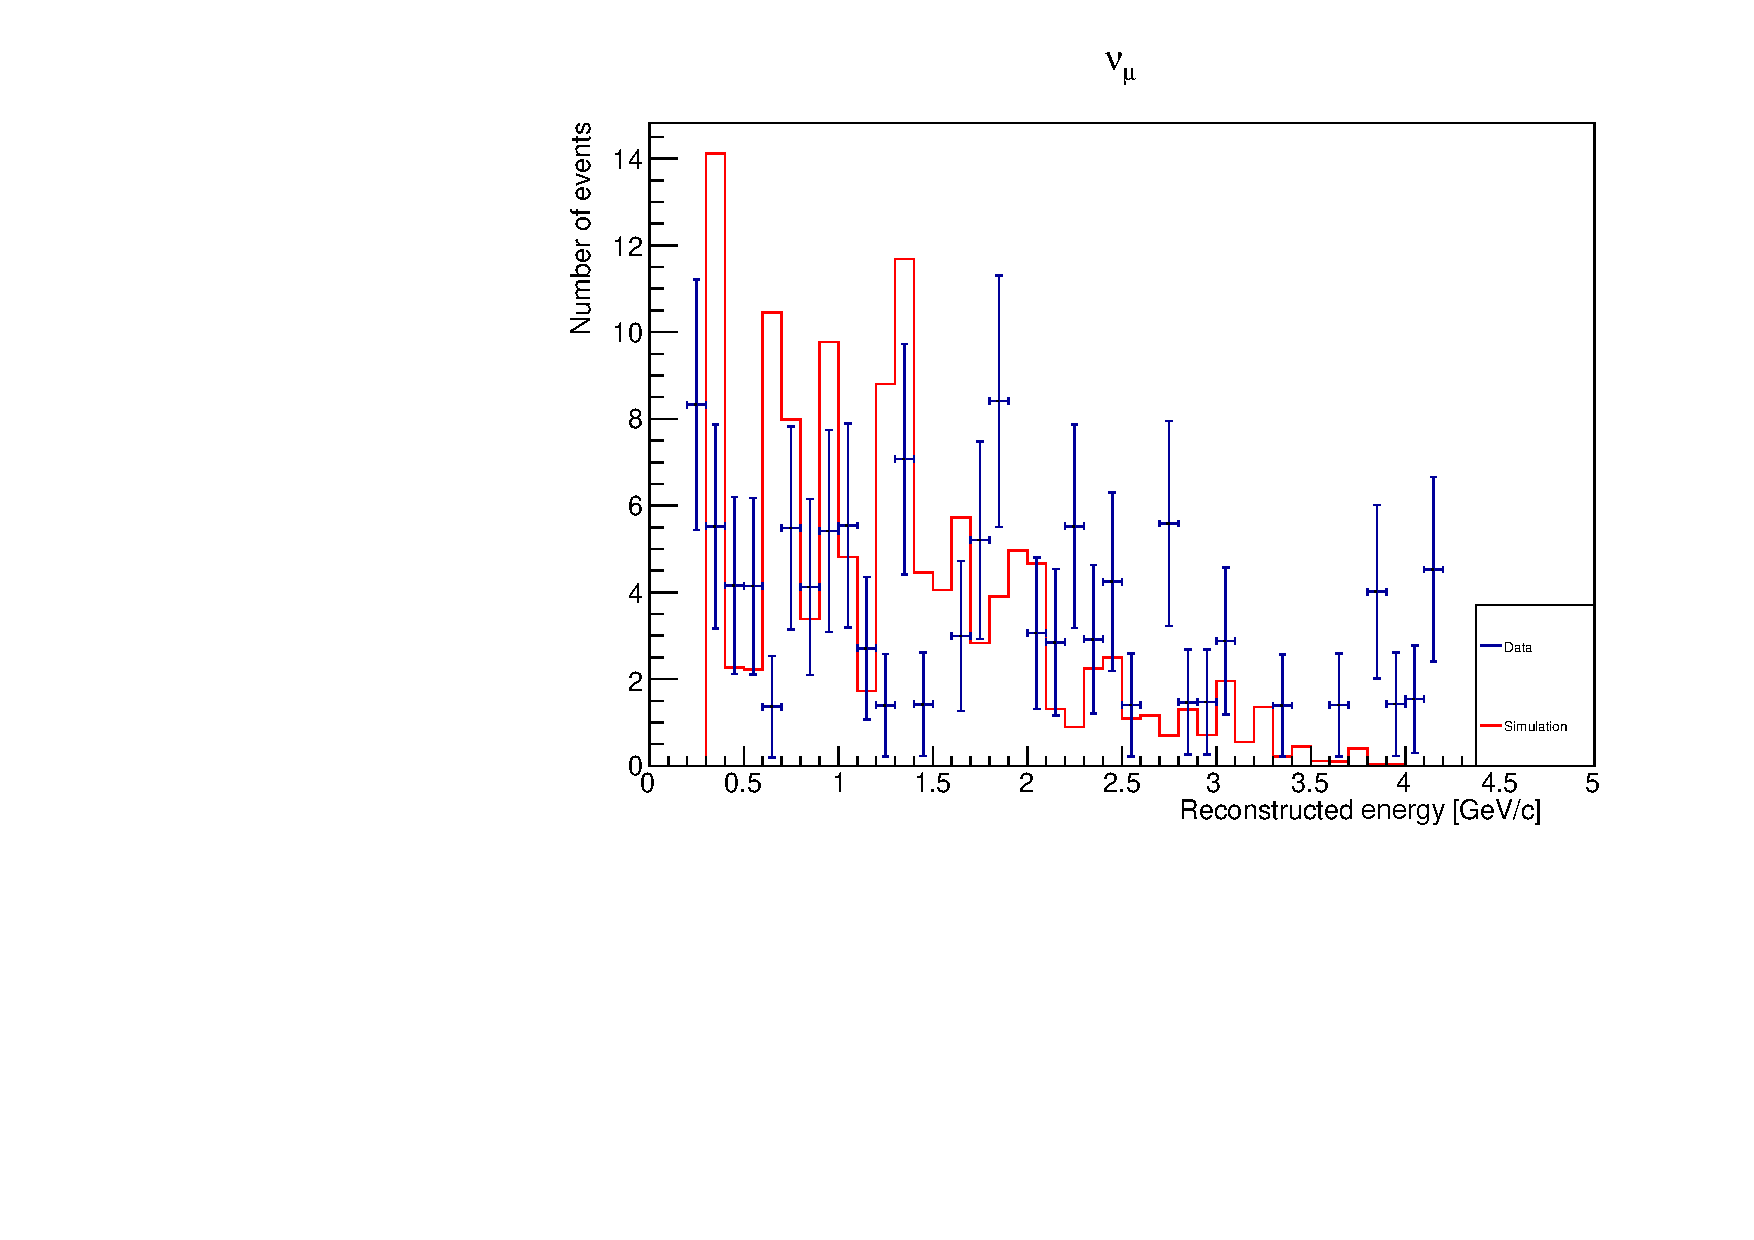
\includegraphics[width=.9\textwidth]{figures/NeutrinoChap/nuEventNewest.pdf}
\caption{Energy spectrum of the reconstructed neutrino $\nu_\mu$ events in data (points with error bars) compared to the simulation (histogram).}
\label{fig:datanumu}
\end{figure}



%\pagebreak
%\section{Future studies}

%\subsection{Interactions in the full WAGASCI}

%Using WAGASCI as a CCQE identification, perhaps even using some of the INGRID modules to provide range momentum reconstruction at the very low momentum.


%\subsection{Neutrino interactions in WAGASCI + Baby MIND}








%Discuss future data taking, interactions everywhere etc etc.

%\subsection{GAr + BabyMIND}
%\subsubsection{Analysis Simulations}
%\subsection{TASD + BabyMIND}
%\subsubsection{Analysis Simulations}
%\subsection{Full WAGASCI}
%\subsubsection{Analysis with Simulations}
%\subsubsection{Simulations vs data}

%\section{Electron charge current quasi-elastic}

\section{Summary}
During commissioning of Baby MIND, it was possible to reconstruct neutrino events during the data taking period in May 2018. A preliminary study was carried out to reconstruct neutrino interactions in the first three iron plates of Baby MIND and measure neutrino and antineutrino events from the Reverse Horn Current beam at a 1.5$^\circ$ off-axis angle. Charge reconstruction was achieved, with momentum measurements down to 400 MeV/c. A total of 224 neutrino and antineutrino events were identified in  Baby MIND, which are the first neutrino events observed in this detector.
